\documentclass[a4paper,11pt]{book}
\usepackage[T1]{fontenc}
\usepackage[utf8]{inputenc}
\usepackage{lmodern}

\usepackage{makeidx}
    % Needed to build the index.

\usepackage{amsmath}
    % Brings the align environment for lining up equations on the =.

\usepackage{amssymb}
    % For the number set symbols.

\usepackage{cancel}
    % For striking out bits of equations that simplify.

\usepackage{graphicx}
    % Can't have pictures/photos/figures from files without that.
    % Note that vanilla latex will only accept eps.
    
\usepackage{subfigure}
    % Lets me have labels such as a) b) c) inside a figure environment.

\usepackage[font=footnotesize, labelfont=bf]{caption}
    % So that I can add long captions under figures.
    % It provides me with \caption* that does not appear in the list of
    % figures but formats the text like \caption does.  It also lets me
    % use line breaks in the caption, and even bullet/enumerated lists.

\usepackage{color}
    % For rendering text is eps_tex files produced by InkScape, even
    % if the text is black.

\usepackage{booktabs}
    % For professional-looking tables.
    % Brings the \toprule, \midrule and \bottomrule.
    % Remember not to use vertical rules in tables: they look cheap.

\usepackage[version=3]{mhchem}
    % For chemical formulas.
    % Brings \ce.ormulas.

\usepackage[mediumspace,mediumqspace,squaren]{SIunits}
    % Otherwise I can't write the mu symbol for micrometers.
    % It also brings me the \degree symbol, woo!
    % No decibel though, I need to make this one myself.

\usepackage{stmaryrd}
    % For the llbracket and rrbracket to denote integer intervals.

\usepackage{algorithmic}
    % For pseudocode.
\usepackage[chapter]{algorithm}
    % To float algorithms.

\usepackage{varioref}
    % For fancier references that also tell the page number.
    
\usepackage{todonotes}
    % Big post-its, handy while writing.
    
\usepackage[]{biblatex}
    % Fantastic bibliography manager that I'll use just for its
    % \citetitle command.

\newcommand{\decibel}{dB}
\newcommand{\equaldef}{\stackrel{\text{\tiny def}}{=}}
\newcommand{\transp}{^T}
\newcommand{\norm}[1]{\left\| #1 \right\|}
\newcommand{\abs}[1]{\left| #1 \right|}


\setcounter{secnumdepth}{3}
    % Number the subsubsections too, as the default stops at subsections.
\setcounter{tocdepth}{5}
    % Table of content goes down to the subparagraphs.

\title{The effect of standing waves on the calibration of heterodyne receivers.}
\author{Bertrand Delforge}

\makeindex
\addbibresource{bibliography.bib}

\newcommand{\MyGraphicsPath}{../../figures/}
\graphicspath{{\MyGraphicsPath}}
\DeclareGraphicsExtensions{.pdf,.jpeg,.png}

\begin{document}
\frontmatter
\maketitle
\tableofcontents
\newpage

\listoffigures
\listofalgorithms
\newpage

\clearpage
\chapter{Abstract}
Put abstract here.

\clearpage
\chapter{Acknowledgements}
Put acknowledgements here.
\mainmatter

\cleardoublepage
\chapter{Introduction to standing waves and HIFI}
\cleardoublepage
\chapter{Introduction to standing waves and HIFI}
Standing waves are a result from interferences, and interferences are a consequence of coherence.

\section{Coherence and interference}
The mixer receives power from many sources:
\begin{itemize}
    \item the LO signal, high power phase-locked monocromatic, reference of the phases, coherent by design;
    \item the sky signal in both sidebands, a priori incoherent;
    \item noise from the LO, a priori incoherent;
    \item black body radiation from the calibration loads, a priori incoherent;
    \item other sources of noise, thermal or not, a priori incoherent.
\end{itemize}
A priori the useful LO signal is coherent and all the other sources behave like noise.
However, the high frequency resolution of the instrument makes these noise sources coherent.

The coherence time~$\tau$ of a signal is inversely proportional to its bandwidth~$\Delta f$:
the narrower the bandwidth, the longer the signal remains in phase, as illustrated by \cref{fig:coherence}.
\begin{figure}[hbtp]
    \centering
    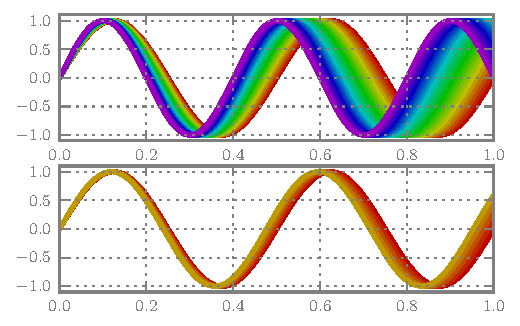
\includegraphics{coherence}
    \caption{
        Signals with a narrow bandwidth remain in phase longer.
        Colors represent frequencies.
        The $x$ axis can represent either time or space and the $y$ axis represents the amplitude of the electric field for the corresponding frequency.
        After propagating to $x=0.85$, the red and purple frequencies of the top-plot signal have opposite phase; a detector that cannot discriminate between them adds up their contribution to 0.
        In the bottom plot, the signal is still very much in phase at $x=0.85$
        because it has a narrower bandwidth.
    }
    \label{fig:coherence}
\end{figure}

Each WBS channel has a bandwidth $\Delta f = \SI{1.1}{\mega\hertz}$,
which yields $\tau = 1 / \Delta f = \SI{909}{\nano\second}$.
By multiplying by the speed of light, we find that the WBS has a coherence length of~\SI{273}{\meter}.
This means that, as long as a signals travels significantly less than~\SI{273}{\meter}, it is coherent as far as the WBS is concerned.
The pathlengths inside HIFI are much shorter than~\SI{273}{\meter}.
For example, the distance between the LOs and the mixers are about~\SI{1}{\meter}.
In that context, all the sources of noise in HIFI are coherent.

Coherence makes you care about the phase, and also about the polarization.

Explain interference.

Show that incoherent systems do not have to care.
Incoherent system: no phase information, just power.
Incoherent system can still have polarization, but they can be unpolarized.
Coherent system are always polarized.






\section{Cavities}
Two reflective surfaces facing each other form a cavity.
At least one of the two surfaces must be partly transparent so that the light can enter and exit the cavity.
The light that enters the cavity can come out after any number $N$ of round trips.
If the distance between the surfaces is $d$, the length of a round trip is $2d$.
After $N$ round trips, a wave of wavelength $\lambda$ is dephased by $2\pi N2d/\lambda$ radians.

The wave inside the cavity is a superposition of the infinite number of waves traveling in both directions (for $N=1$ to $\infty$).
That wave is a ``standing wave'', its nodes and crests do not propagate in space.
We do not observe standing waves directly, but we observe the effect of interferences.
Standing waves are an other effect of these same interferences.

Whenever $N2d/\lambda$ is an integer, all the waves exiting the cavities have the same phase, we have resonance and constructive interference.
This condition is verified for $2d=M\lambda$ with $M$ an integer, that is when the length of a round trip is a multiple of the wavelength.
Other values of $\lambda$ produce destructive intereferences, or anything between totally constructive and totally destructive.
The effect that a cavity has on a signal depends on its wavelength.

The spectra measured by the WBS have about 8000 channels, covering frequencies from 4 to \SI{8}{\giga\hertz} with a \SI{0.5}{\mega\hertz} spacing.
Each of these channels has its own frequency, and therefore its own wavelength.
This implies that each channel of the WBS spectrometer has its own coupling coefficient to the various sources of signal in the system, solely due to the cavities in the optics.

If we consider a cavity of length $d=\SI{1.5}{\meter}$ (distance LO--mixer in HIFI), then its fundamental wavelength is $\lambda=2d/M$ for $M=1$, which gives $\lambda=\SI{3}{\meter}$.
That wavelength corresponds to the frequency $f=c/\lambda \approx \SI{100}{\mega\hertz}$.
The harmonics (higher values of $M$) are at \SI{200}{\mega\hertz}, \SI{300}{\mega\hertz}, \SI{400}{\mega\hertz}, \ldots, \SI{921700}{\mega\hertz}, \SI{921800}{\mega\hertz}, etc.  These last two values are near the \transition{CO}{8}{7} transition (\cref{table:co_transition_frequencies}).

It should now be clear that any two frequencies separated by \SI{100}{\mega\hertz} are dephased in the same way by a \SI{1.5}{\meter}-long cavity.
In other words, that cavity introduces periodic modulations of the coupling coefficient of the mixer, which produces periodic patters on the measured spectrum.

Ideally the calibration should take care of standing waves, but it does not.
Indeed, the calibration of HIFI requires integrating on the internal hot and cold black bodies.
This means changing the optical configuration of the instrument, as the chopper turns to select the source, and the black bodies are partly reflective.
In a (on-off)/(hot-cold) calibration scheme, the standing waves in the hot and the cold do not cancel each other, nor do they cancel the standing waves in the on and off phases.
By using different optical paths during a single observation, and by not having an adequate model of these optical paths, we introduce standing wave artifacts in our spectra.

\begin{figure}[htbp]
    \centering
    \includegraphics{mars_50010cb7_WBSH_USB}
    \caption{
        The modulation of this spectrum of Mars indicates the presence of cavities in the optical system.
    }
    \label{fig:mars}
\end{figure}

Sometimes, the effects are obvious, like on the spectrum of Mars in \cref{fig:mars}.
The period of this periodic pattern indicates a cavity approximately \SI{1.5}{\meter}-long, which can be mixer--LO, mixer--CBB or mixer-HBB, most likely of mix of the three.
CBB and HBB stand for ``Cold Black Body'' and ``Hot Black Body'', two internal calibration sources.

Often, the modulation are barely noticeable by visual inspection but can have a considerable impact on the astronomical interpretation, as we will show in \cref{sec:chapter5}.

\todo[inline]{
Low Q and high Q: sine is an approximation that works only at low Q.
}

\subsection{Cavity period}
\begin{equation}
    F = \frac{c}{2d} \label{eq:cavity_period}
\end{equation}


\section{The Heterodyne Instrument for the Far Infrared}

Keywords: Heterodyne, double sideband, sideband ratio.

The HIFI instrument on the Herschel Space Observatory~\cite{AA_518_L1} is a heterodyne receiver that operates at frequencies between \SI{480}{\giga\hertz} and \SI{1910}{\giga\hertz},
producing spectra with a resolution ranging from \SI{1}{\mega\hertz} to \SI{125}{\kilo\hertz}~\cite{AA_518_L6}.
This high frequency resolution enables the astronomers to study the chemistry of a wide range of phenomena, from planetary atmospheres to star forming regions.

At such a high resolution, the thermal noise of the astronomical source, the calibration black bodies and the local oscillator (LO) qualify as ``narrow band Gaussian noise signals''~\cite{siegman1986lasers}.
They have a coherence time~$\tau$ equal to the inverse of their bandwidth~$\tau=1/\Delta f$.
A bandwidth of~\SI{1}{\mega\hertz} results in a coherence time of~\SI{1}{\micro\second} equivalent to a coherence length of~\SI{300}{\meter}.
This is a hundred times the longest distance inside HIFI.
Therefore, in HIFI, the signals from the LO, the calibration sources and the sky are coherent.

Show spectra with standing wave patterns.



\section{The sideband ratio problem}

Explain how we perform the flux calibration.
Explain how it cannot cancel all the standing waves.
Explain how the dual sideband aspect makes things difficult: many more variables but not more equations.
This is where the sideband ratio comes into play: it connects the LSB and USB gains, reducing the number of independant variables in the system.

Because of the lack of equations, the sideband ratio cannot be retreived from the data and, instead, must be assumed.
This is the motivation of my model.

Show that, by looking at their period, we determined a while ago the cavities responsible.
Point to the cavities on drawing.
Tells that it imposes welcome constraints on our model.



\section{Modeling standing waves}
It is not really about modelling standing waves, it is about modeling coupling.
Standing waves are taken care of during the process.

In brief, the general ideas of how my model works, and why.
This includes some confession regarding simplifications.

Conclude that the method in this thesis can be applied to any single-mode coherent system.
Lasers are good candidates.



\section{Applications to astronomy}


\cleardoublepage
\chapter{Computing standing waves}
\cleardoublepage
\chapter{Computing standing waves}
\label{sec:chapter2}
\section{Principle}
Our method is inspired from laser and circuit theory: we deal with discrete inputs and outputs rather than, for example, a spatial description of the fields.
A system like the Focal Plane Unit of HIFI comprises a few dozens of optical elements~\cite{jackson2002hifi}, referred in the literature as ``networks''~\cite{siegman1986lasers}: wire grid polarizers, roof-top mirrors, horns, attenuators, free space, all having one or more input and output.
All these networks interact together two by two since there exists at least one optical path between each pair or networks.
The number of interactions in the system increases faster than the square of the number of networks.
One way to solve a system's reaction to a set of input would be to propagate the inputs from network to network, back and forth, until the fields appear to converge to a steady state.
Instead, we propose a method to that directly provides the steady state.

%#############################################################################
\section{Solver}

%=============================================================================
\subsection{Simplifications}

Plane wave.
Single mode.

Not only a list, I must justify them.
Anything below -40 dB can pretty much be ignored \todo{why?}.
What does not couple is lost, so just model the higher modes with a loss parameter.
This is going to work unless higher modes can come back to the fundamental mode, but that should be a very small effect.



%=============================================================================
\subsection{Conventions and definitions}
Equations \eqref{eq:e_z_t_real_minus} and \eqref{eq:e_z_t_real_plus} are two equivalent expressions of the amplitude of the electric field of a plane wave propagating along an axis~$\vect{z}$.
These two expressions are equivalent because the $\cos$ function is even.
Choosing one or the other is a matter of convention.
\begin{subequations}
    \begin{align}
       E(z, t) &= E_0 \cos( kz - \omega t + \varphi)   \label{eq:e_z_t_real_minus} \\
       E(z, t) &= E_0 \cos(-kz + \omega t - \varphi)   \label{eq:e_z_t_real_plus}
    \end{align}
    \label{eq:e_z_t_real}
\end{subequations}
\Cref{eq:e_z_t_real} is illustrated \cref{fig:plane_wave_propagation} as a function of~$z$ for a few values of~$t$.
\begin{figure}[hbp]
    \centering
    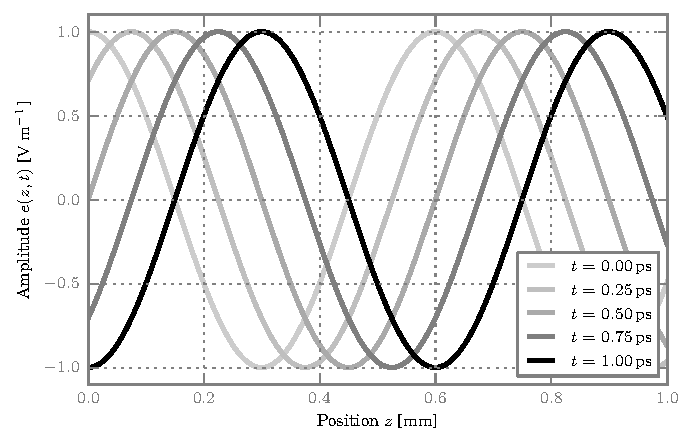
\includegraphics{plane_wave_propagation}
    \caption {\label{fig:plane_wave_propagation}Electric field amplitude of a wave of frequency \SI{500}{\giga\hertz} and amplitude \SI{1}{\volt\per\meter} propagating in vacuum (refractive index 1).}
\end{figure}

In \cref{eq:e_z_t_real}, $t$ is the time coordinate and~$z$ the space coordinate.
$\varphi$ is related to initial conditions and the choice of reference frame.
$E_0$ is the amplitude of the electric field.
It has the dimension of an electric potential per unit length.
It is given for example in volts per meter or newtons per coulomb.

\begin{table}
    \centering
    \caption{Notations and definitions of electromagnetic constants and parameters}
    \caption*{All the entries in this table are real numbers.}
    \label{tab:definitions_simple}
    \rowcolors{2}{gray!25}{white}
    \begin{tabularx}{\textwidth}{l l X}
        \toprule
        \hiderowcolors
        notation & definition & name \\
        \showrowcolors
        \midrule
        $\omega$      &  $2 \pi f$   &  angular frequency \\
        $k$           &  $2 \pi / \lambda$   &   wave number or angular frequency\\
        $\lambda$     &  $c / f$  &  wavelength \\
        $c$           &  $c_0 / n$  &  phase velocity \\
        $c_0$         &  $=\SI{299792458}{\meter\per\second}$  &  speed of light in vacuum \\
        $n$           &  $\sqrt{\epsilon_r \mu_r}$  &  refractive index \\
        $\epsilon_r$  &  $\epsilon / \epsilon_0$  &  relative permittivity or electric constant\\
        $\mu_r$       &  $\mu / \mu_0$  &  relative permeability or magnetic constant\\
        $\epsilon$    & measured material property & absolute permittivity \\
        $\mu$         & measured material property & absolute permeability \\
        $\epsilon_0$  & $\approx \SI{8.854187817e-12}{\farad\per\meter}$  &  absolute permittivity of vacuum \\
        $\mu_0$       & $\approx \SI{1.2566370614e-6}{\henry\per\meter}$  &  absolute permeability of vacuum \\
        $\eta$        & $\sqrt{\mu / \epsilon}$  &  intrinsic impedance \\
        $\eta_0$      & $\sqrt{\mu_0 / \epsilon_0}$  &  intrinsic impedance of free space \\
        $Z$           & $E / H$  & wave impedance \\
        \bottomrule
    \end{tabularx}
\end{table}

\Cref{tab:definitions_simple} summarizes the relations between various parameters used to describe a wave and its propagation medium.
For plane waves in homogeneous materials, $Z=\eta$.
All the parameters introduced in this table are real numbers.
It is possible to add more parameters, such as the electric conductivity of a material.
Such parameters account for attenuation, phase delays, etc.
However, these are more easily dealt with when using complex numbers without changing any of these equations.
In \cref{sec:polar_complex_notation}, we will go over these parameters again and explore the effects of giving them an imaginary part.


%=============================================================================
\subsection{Polar complex notation}
\label{sec:polar_complex_notation}
Euler's formula, given in \cref{eq:euler_formula}, relates the trigonometric function $\cos$ to a complex exponential.
\begin{equation}    
    \exp(i\theta) = \cos(\theta) + i\sin(\theta) \label{eq:euler_formula}
\end{equation}
In \cref{eq:euler_formula}, $i$ represents the imaginary unit such that $i^2=-1$.
If we rewrite the expression of~$E$ given in \cref{eq:e_z_t_real_minus} as a complex in polar coordinates, we have \cref{eq:e_z_t_complex_minus}.
\begin{align}
   \hat{E}(z, t) &= E_0 \exp(i(kz - \omega t + \varphi))
   \label{eq:e_z_t_complex_minus}
   \\
   E(z, t) &= \Re(\hat{E}(z, t))
   \label{eq:e_z_t_real_complex_minus}
\end{align}
The hat above the $E$ signals that $\hat{E}$ is the complex equivalent of $E$.
As shown by \cref{eq:e_z_t_real_complex_minus}, $E$ and $\hat{E}$ do not have the same value (one is real, the other is complex);
however, both describe the same physical phenomenon.

If we open the door to complex numbers, we may want to consider the effect of giving an imaginary part to the parameters of \cref{tab:definitions_simple}.

The imaginary part of the complex angular frequency $\hat{\omega} = \omega' + i \omega''$ corresponds to an amplification of the wave in time, see \cref{eq:complex_angular_frequency}.
If the imaginary part is negative, then the effect is an attenuation of the signal as time goes.
\begin{subequations}
    \begin{align}
       \hat{E}(z, t) &=
       E_0 \exp(i(kz - \hat{\omega} t + \varphi))
       \\
       &=
       E_0 \exp(i(kz - (\omega' + i \omega'') t + \varphi))
       \\
       &=
       E_0 \exp(i(kz - \omega' t + \varphi)) \exp(\omega'' t)
    \end{align}
    \label{eq:complex_angular_frequency}
\end{subequations}
This can be used to model systems that vary in time.
Since the systems we study in this book are time-invariant, $\omega$ will always be real for us.

Folowing the same reasoning, the imaginary part of the complex wavenumber $\hat{k} = k' + i k''$ corresponds to a spatial attenuation or amplification.
See \cref{eq:complex_wavenumber}.
If $k''> 0$, then the wave is attenuated as it propagates.
This can model losses in a material.
\begin{subequations}
    \begin{align}
       \hat{E}(z, t) &=
       E_0 \exp(i(\hat{k}z - \omega t + \varphi))
       \\
       &=
       E_0 \exp(i((k' + i k'')z - \omega t + \varphi))
       \\
       &=
       E_0 \exp(i(k' z - \omega t + \varphi)) \exp(-k'' z)
    \end{align}
    \label{eq:complex_wavenumber}
\end{subequations}
Having $k'' \ne 0$ gives an imaginary part to the wavelength and the phase velocity
(see \cref{tab:definitions_simple}).
All these imaginary parts mean the same thing: the wave is getting attenuated.
However, the speed of light in vacuum is known to be a real number.
Therefore, the imaginary part of $\hat{k}$ comes from an imaginary part of the complex refractive index $\hat{n}$.
This links the attenuation of the wave to a property of the material.
Since the refractive index is derived from the relative electric permittivity and the relative magnetic permeability of a materials
($\hat{n}=\sqrt{\hat{\epsilon}\hat{\mu}}$),
any of them can be responsible for the attenuation of the wave.

When using Snell's law \eqref{eq:snell}, the real part of the refractive indices must be used.

In many cases (vacuum, mylar, aluminum), the relative magnetic permeability is very close to 1, making the electric permitivity the only parameter able to bear an imaginary part.
This means that, in these cases, the wave is absorbed by a material because of its conductivity.
The conductivity $\sigma$ and the imaginary part of the permittivity $\epsilon''$ are bound by \cref{eq:epsilon_second_sigma}.
The higher the frequency, the less effect the conductivity has.
This is understandable as inertia prevents the electrons from moving fast enough to cancel the electric field.
\begin{equation}   
    \epsilon'' = \sigma / \omega
    \label{eq:epsilon_second_sigma}
\end{equation}
The conductivity itself can be complex, in which case its imaginary part acts like a frequency-dependant real part of the permittivity.

In some cases, the relative magnetic permeability is very different from~1 and is able to go up to several thousands in the case of very pure iron.
It can a priori be complex.
\citeauthor{bowler2006frequency} has shown in \citetitle{bowler2006frequency} \cite{bowler2006frequency} that the imaginary part of the permeability is frequency dependant.
However, that frequency dependance of $\mu''$ does not seem as simple as that of $\epsilon''$.

Finally, the complex intrinsic impedance derived from the complex permittivity and permeability imply that the electric and magnetic fields are not in phase.
Indeed, for a plane wave in a homogeneous material, the wave impedance $\hat{Z}=\hat{E}/\hat{H}$ equals the intrinsic impedance $\hat{\eta}=\sqrt{\hat{\mu}/\hat{\epsilon}}$.
Therefore, the imaginary part of $\hat{\mu}$ or $\hat{\epsilon}$ creates a phase difference between $\hat{E}$ and $\hat{H}$.

%=============================================================================
\subsection{Phasors}
\index{phasor}

\subsubsection{Introducing phasors}
By applying the exponentiation identity \cref{eq:exponentiation_identity},
\cref{eq:e_z_t_complex_minus} can also be written as \cref{eq:e_z_t_complex_factorized}.
\begin{equation}
    \exp(a+b) = \exp(a) \exp(b)
    \label{eq:exponentiation_identity}
\end{equation}
\begin{equation}
    \hat{E}(z, t)
    =
    E_0 \exp(ikz) \exp(-i\omega t) \exp({i \varphi})
    \label{eq:e_z_t_complex_factorized}
\end{equation}
In \cref{eq:e_z_t_complex_factorized}, the expression of the wave is separated into four independant factors.
This is possible because the amplitude $E_0$, the wavenumber $k$, the angular frequency $\omega$ and the phase $\varphi$ are time-invariant.
The time-invariance of $\omega$ and $k$ is guaranteed by the linearity hypothesis, while that of $E_0$ and $\varphi$ is guaranteed by the coherency hypothesis.

The time factor $\exp({-i \omega t})$ is common to all the waves present in the system.
Because of that, we can factor it out as shown in equations~\ref{eq:factor_time_out} and \ref{eq:phasor}.
In these equations, $\hat{E}(z)$ is a ``phasor representation'' of the sinusoidal function $E(z, t)$, with the time factored out and considered implicit.
\begin{align}
    \hat{E}(z, t) &= \hat{E}(z) \exp(-i\omega t) \label{eq:factor_time_out}
    \\
    \hat{E}(z) &= E_0 \exp(i(kz+\varphi)) \label{eq:phasor}
\end{align}

The term ``phasor'' is a portmanteau of ``phase vector'', indicating that $\hat{E}(z)$ can be visualized as a vector on the complex plane, and that $\hat{E}(z, t)$ makes that vector rotate with time.

\subsubsection{Convention}
We have shown with equations~\ref{eq:e_z_t_real_minus} and \ref{eq:e_z_t_real_plus} that there are two conventions for representing the same physical phenomenon.
Either the space factor or the time factor takes a negative sign, and that decision is a priori arbitrary.

The choice of convention influences the definition of our phasors.
We have to choose between
\cref{eq:phasor_minus} and \cref{eq:phasor_plus}.
\begin{subequations}
    \begin{align}
        \text{Either }
        \hat{E}(z) &= E_0 \exp(i(kz+\varphi))
        \label{eq:phasor_minus}
        \\
        \text{or }
        \hat{E}(z) &= E_0 \exp(i(-kz-\varphi))
        \text{.}
         \label{eq:phasor_plus}
    \end{align}    
\end{subequations}

For simplicity, we choose \cref{eq:phasor_minus}.
Indeed, it does not carry a negative sign.
The negative sign is factored out in the time-factor $\exp{-i \omega t}$.


\subsubsection{Discrete space}
In our optical systems, we are hardly ever interested in the value of the phasor at any point.
For example, when modeling the effect of a dielectric interface on a wave, we need only to know the value of the phasor at the location of the interface.
If there are two interfaces, then there are two points of interest.
This means that we do not keep the explicit dependency on $z$ in our computations but work with discrete values of $z$ as illustrated by \cref{eq:phasor_no_z}.
\begin{equation}
    \begin{aligned}
        \hat{E}_0 &= E_0 \exp(i(k_0 z_0 + \varphi_0))
        \\
        \hat{E}_1 &= E_1 \exp(i(k_1 z_1 + \varphi_1))
    \end{aligned}
    \label{eq:phasor_no_z}
\end{equation}
In \cref{eq:phasor_no_z}, the phasors $\hat{E}_n$ do not depend on a space coordinate because they are defined for a specific location.
This is the type of phasors that we will be using in the rest of our chapter.

\subsubsection{Phasor algebra}
Phasors can be added together to produce a new phasor.
Physically, this corresponds to adding together the electric fields of different waves.
This is by adding phasors that we model interferences.

A phasor can be multiplied by a scalar to produce a new phasor.
The scalar can be a complex number, but that does not make this scalar a phasor. 
The real part of the scalar models the gain or absorption, while the imaginary part models the phase shift.
The scalar multiplication models the effect of an optical element on a wave.

Phasors cannot be multiplied together.
In algebraic terms, phasors form a vector space, not a ring.
The product of two phasors would represent the product of two sinusoids which is a non-linear operation that introduce new frequencies.
Since phasors can represent systems with one frequency only, the result of multiplying two phasors is not a phasor.
This means that computing the power transported by a wave is more subtle than just squaring the phasor, which we will study in \vref{sec:jones_vectors_and_power}.


%=============================================================================
\subsection{Scattering matrices}
Scattering matrices \cite{siegman1986lasers} model the transfer of power or field from one side (port) of a network to another (\cref{fig:scattering_matrix_notations}).
In coherent systems, they operate on phasors and therefore manipulate the field, not the power.

\Cref{eq:scattering_matrix} presents the scattering matrix $S$ that models the relation between a vector of inputs $a$ and a vector of outputs $b$ for a $n$-ports network.
The diagonal contains the reflections terms and the rest contains the transmissions.
\begin{align}
    b &= S a
    &
    \begin{pmatrix}
        b_1\\
        b_2\\
        \vdots\\
        b_n
    \end{pmatrix}
    &=
    \begin{pmatrix}
        S_{1, 1} & S_{1, 2} & \cdots & S_{1, n} \\
        S_{2, 1} & S_{2, 2} & \cdots & S_{2, n} \\
        \vdots   & \vdots   & \ddots & \vdots   \\
        S_{n, 1} & S_{n, 2} & \cdots & S_{n, n}
    \end{pmatrix}
    \begin{pmatrix}
        a_1\\
        a_2\\
        \vdots\\
        a_n
    \end{pmatrix}
    \label{eq:scattering_matrix}
\end{align}

\begin{figure}[hbtp]
    \centering
    \input{scattering_matrix_notations.pdf_tex}
    \caption{A 4-ports network showing 4 inputs $a_i$ and four outputs $b_i$.  For example, this network could be a wire grid polarizer or a semi-transparent mirror, both acting as beam splitters.}%
    \label{fig:scattering_matrix_notations}
\end{figure}

In the general case, scattering matrices cannot be multiplied together.
The scattering matrix of a system of two networks is not the product of the scattering matrices of the individual networks.
We will explore this further in \cref{sec:solving_a_system}.

Scattering matrices are firstly designed to model discrete physical optical elements such as interfaces, distances, horns, grids, etc.
It is possible to extend their use to an entire system made of several networks as long as it provides outputs that are linear combinations of inputs.
We will also explore this further in \cref{sec:solving_a_system}.



%=============================================================================
\subsection{Jones calculus in 3D}

%-----------------------------------------------------------------------------
\subsubsection{Traditional Jones calculus}
Jones matrices model the transfer of amplitude and phase from one polarization to another \cite{hecht2002optics}.
In \cref{eq:jones_matrix_short}, the polarized input field $\vect{\hat{E}}_i$ is related to the polarized output field~$\vect{\hat{E}}_o$ by the Jones matrix $J$.
$\vect{\hat{E}}_i$ and $\vect{\hat{E}}_o$ are called ``Jones vectors''.
\begin{equation}
    % Small form.
    \vect{\hat{E}}_o = J \vect{\hat{E}}_i
    \label{eq:jones_matrix_short}
\end{equation}
The components of the Jones vectors are phasors: complex numbers that encode the amplitude and phase of the field along different axes.
The components of the Jones matrices are als numbers, these encode changes in amplitude and phase.

\Cref{eq:jones_matrix_2d} presents the traditional form of Jones vectors and matrices.
\begin{equation}
    % Jones matrix in 2D.
    \begin{pmatrix}
        \hat{E}_{o, h}\\
        \hat{E}_{o, v}
    \end{pmatrix}
    =
    \begin{pmatrix}
        J_{h, h}   &   J_{h, v} \\
        J_{v, h}   &   J_{v, v}
    \end{pmatrix}
    \begin{pmatrix}
        \hat{E}_{i, h}\\
        \hat{E}_{i, v}
    \end{pmatrix}
    \label{eq:jones_matrix_2d}
\end{equation}
The field is seen as the superposition of a horizontal and a vertical component, both linearly polarized.
The phase difference between these components determines the handedness and the ellipticity of the polarization of the field.

%-----------------------------------------------------------------------------
\subsubsection{Extension to three dimensions}
Although very useful for many applications, the traditional Jones matrices and vectors have limitations.
First, the field is always expressed in a local reference frame: the horizontal and vertical directions are valid for one beam only and may change after any reflection or refraction.
Therefore, to completely describe a field, the Jones vector is not enough since one needs to keep track of the orientation of its reference frame with three angles, a quaternion or a rotation matrix.

Second, the horizontal and vertical directions are normal to each other and to the direction of propagation.
This limits us to modeling either transverse electric or transverse magnetic waves depending on whether the Jones vector represents the electric or the magnetic field;
this cannot model hybrid waves, in which both the electric and the magnetic field can have a component along the direction of propagation.
Therefore, this cannot model propagation in a birefringent material.
One way to accommodate this is to relax the constraint of orthogonality of the reference frame, allowing for the horizontal and vertical directions to have a component along the direction of propagation.
If we do this, then the full description of the field gets even more complicated as we need to carry along, not just the orientation of its reference frame, but the full description of that non-Cartesian reference frame.

Instead, we can express all the fields in a common global Cartesian reference frame, essentially extending Jones calculus from two to three dimensions, as illustrated in \cref{eq:jones_matrix_3d}.
\begin{equation}
    % Jones matrix in 3D.
    \begin{pmatrix}
        \hat{E}_{o, x}\\
        \hat{E}_{o, y}\\
        \hat{E}_{o, z}
    \end{pmatrix}
    =
    \begin{pmatrix}
        J_{x, x}   &   J_{x, y}   &   J_{x, z} \\
        J_{y, x}   &   J_{y, y}   &   J_{y, z} \\
        J_{z, x}   &   J_{z, y}   &   J_{z, z}
    \end{pmatrix}
    \begin{pmatrix}
        \hat{E}_{i, x}\\
        \hat{E}_{i, y}\\
        \hat{E}_{i, z}
    \end{pmatrix}
    \label{eq:jones_matrix_3d}
\end{equation}
These Jones matrices can be combined with rotation matrices (built from Euler angles or quaternions) in order to represent networks in any orientation in space.

%-----------------------------------------------------------------------------
\subsubsection{Rotating Jones matrices}
\label{sec:rotating_jones_matrices}
If $R$ is a 3--by--3 rotation matrix and $J$ the Jones matrix of a network at rest,
then \cref{eq:jones_rotation_using_inverse} gives the Jones matrix $J'$ corresponding to that network rotated by $R$.

\begin{equation}
    J' = R J R^{-1}
    \label{eq:jones_rotation_using_inverse}
\end{equation}
\Cref{eq:jones_rotation_using_inverse} is correct, however it may not be the most practical to implement.
Indeed, inverting matrices is an expensive and unstable operation for a computer to perform
When we remember that the inverse of a rotation matrix is also its transpose%
\todo{citation needed},
then we get \cref{eq:jones_rotation_using_transpose} which has the advantage of being computationally cheap and stable.
\begin{equation}
    J' = R J R\transp
    \label{eq:jones_rotation_using_transpose}
\end{equation}

Rotating the identity matrix has an interesting property shown by~\eqref{eq:jones_rotation_identity}.
\begin{equation}
    I' = R I R^{-1}
       = R R^{-1}
       = I
    \label{eq:jones_rotation_identity}
\end{equation}
If a Jones matrix is proportional to an identity matrix, then it is not modified by rotation.
We will use that property to save some computation, for example when propagating through homogeneous isotropic materials (\vref{sec:generic_networks_distance}).



%=============================================================================
\subsection{Jones vectors and power}
\label{sec:jones_vectors_and_power}
When dealing with complex numbers, we must carefully define what we mean by ``power''.
\citetitle{IEEE2002dictionary} \cite{IEEE2002dictionary} defines the following terms and SI units:
\begin{description}
    \item[complex power]\quad%
    $\hat{S} = P + iQ$\quad%
    in \si{\volt\ampere} (volt-ampere),
    \item[active/real power]\quad%
    $P \in \mathbb{R} = \Re(\hat{S})$\quad%
    in \si{\watt} (watt),
    \item[reactive power]\quad%
    $Q \in \mathbb{R} = \Im(\hat{S})$\quad%
    in \si{var} (volt-ampere-reactive),
    \item[apparent power]\quad%
    $\abs{\hat{S}} = \sqrt{P^2 + Q^2}$\quad%
    in \si{\volt\ampere} (volt-ampere).
\end{description}
In our case, we deal with power densities: instead of watt, we use watt per square meter.
We can define ``complex power density'', ``active power density'', ``reactive power density'' and ``apparent power density'' by taking the correspondant absolute powers from the list above and normalizing them by a unit surface area.
For simplicity, we keep the same notations.

Considering that the electric field is given in volt per meter and the magnetic field in ampere per meter, their product yields a quantity that has the dimension of a power density.
It is tempting to write $\hat{S}=\hat{E}\hat{H}$ with $\hat{E}$ and $\hat{H}$ phasors;
however this is incorrect for two reasons:
\begin{enumerate}
    \item each phasor represents a sinusoidal signal, and the product of two sinusoids is a non-linear operation that introduces new frequencies,
    \item our electric and magnetic fields are three dimensional, they are Jones vectors.
\end{enumerate}

\index{Poynting vector}The ``Poynting vector'' represents the directional energy flux density of an electromagnetic wave, typically expressed in \si{\watt\per\meter\squared}.
Traditionally noted~$\vect{S}$, it is defined by \cref{eq:poynting_vector}.
This vector takes care of the fact that the electric and magnetic fields ($\vect{E}$ and $\vect{H}$) are three dimensional vectors.
However, as indicated by the absence of hat symbols, the components of $\vect{E}$, $\vect{H}$ and $\vect{S}$ are real numbers, not complex numbers.
This means that we cannot use phasors directly in this equation.
The letter~$\vect{S}$ here must not be confused with the~$\hat{S}$ above which corresponds to a complex power.
Actually, since the Poynting vector deals with real values, it has more affinities with the active power density $P$.
\begin{equation}
    \vect{S} = \vect{E} \times \vect{H} \label{eq:poynting_vector}
\end{equation}
The definition of this Poynting vector holds even for anisotropic propagation media for which $\vect{E}$, $\vect{H}$ and the wave vector $\vect{k}$ may not be normal to each other.
Since the Poynting vector is defined by a cross product, it is by definition normal to the electric and magnetic field, even if that direction differs from $\vect{k}$.

Since the active power is a priori the most interesting (sources emit real power, and detectors detect real power), let us compute the Poynting vector from $\vect{\hat{E}}$ and $\vect{\hat{H}}$, both three dimentional vectors with phasors components.

In order to avoid non-linearities, the first thing to do is to express the electric and magnetic field with their time factor.
This is shown in \cref{eq:e_h_time}, where the components of $\vect{\hat{E}}(t)$ and $\vect{\hat{H}}(t)$ are not phasors anymore but complex amplitudes.
They are no more representations of sinusoidal functions, they are specific values of these functions.
\begin{subequations}
    \begin{align}
        \vect{\hat{E}}(t) = \vect{\hat{E}} \exp(-i \omega t) \\
        \vect{\hat{H}}(t) = \vect{\hat{H}} \exp(-i \omega t)
    \end{align}
    \label{eq:e_h_time}
\end{subequations}

The second step is to take their real values.
This is what we do with \crefrange{eq:e_time_real_0}{eq:e_time_real_2} for the electric field.
The same equations can be applied to the magnetic field.
These equations are applied on the three components of the vectors independently.
\begin{subequations}
\begin{align}
    \vect{E}(t) &= \Re
    \bigg(
        \Big(
            \Re(\vect{\hat{E}}) + i \Im(\vect{\hat{E}})
        \Big)
        \Big(
            \cos(- \omega t) + i \sin(- \omega t)
        \Big)
    \bigg)
    \label{eq:e_time_real_0}
    \\
    \vect{E}(t) &= \Re(\vect{\hat{E}}) \cos(- \omega t)
            -
            \Im(\vect{\hat{E}}) \sin(- \omega t)
    \label{eq:e_time_real_1}
    \\
    \vect{E}(t) &= \Re(\vect{\hat{E}}) \cos(\omega t)
            +
            \Im(\vect{\hat{E}}) \sin(\omega t)
    \label{eq:e_time_real_2}
\end{align}
    \label{eq:e_time_real}
\end{subequations}

The third step is to compute the cross product of $\vect{E}(t)$ and $\vect{H}(t)$ to get the Poynting vector $\vect{S}(t)$.
For brevity, let us pose $c=\cos(\omega t)$, $s=\sin(\omega t)$,
$\vect{E}_r = \Re(\vect{\hat{E}})$, $\vect{E}_i = \Im(\vect{\hat{E}})$,
$\vect{H}_r = \Re(\vect{\hat{H}})$ and $\vect{H}_i = \Im(\vect{\hat{H}})$.
The Poynting vector is then given by \cref{eq:e_cross_h}.
\begin{equation}
    \vect{S}(t)
    =
    \begin{pmatrix}
         (E_{iy} s + E_{ry} c) (H_{iz} s + H_{rz} c) -
         (E_{iz} s + E_{rz} c) (H_{iy} s + H_{ry} c)
         \\
         (E_{iz} s + E_{rz} c) (H_{ix} s + H_{rx} c) -
         (E_{ix} s + E_{rx} c) (H_{iz} s + H_{rz} c)
         \\
         (E_{ix} s + E_{rx} c) (H_{iy} s + H_{ry} c) -
         (E_{iy} s + E_{ry} c) (H_{ix} s + H_{rx} c)
    \end{pmatrix}
    \label{eq:e_cross_h}
\end{equation}
Expanding the components yields many $\cos(\omega t)^2$, $\sin(\omega t)^2$ and $\cos(\omega t)\sin(\omega t)$.

The Poynting vector is a instantaneous quantity; it is defined for a specific instant $t$.
It is possible to define a time-averaged Poynting vector $\vect{\bar{S}}$ with \cref{eq:pointing_average}.
\begin{equation}
    \vect{\bar{S}} = \frac{1}{T}
    \int_0^T \! \vect{S}(t)\, \mathrm{d}t
    \label{eq:pointing_average}
\end{equation}
In \cref{eq:pointing_average}, $T$ is the period of the signal defined by $T=1/f$ and $f=\omega/2\pi$.
The time-average of the $\sin^2$, $\cos^2$ and $\sin\cos$ functions found in the Poynting vectors are given by \crefrange{eq:trig_average_ss}{eq:trig_average_sc}.
\begin{subequations}
    \begin{align}
        \frac{1}{T} &\int_0^{T} \! \sin(\omega t)^2 \, \mathrm{d}t = \frac{1}{2}
        \label{eq:trig_average_ss}
        \\
        \frac{1}{T} &\int_0^{T} \! \cos(\omega t)^2 \, \mathrm{d}t = \frac{1}{2}
        \label{eq:trig_average_cc}
        \\
        \frac{1}{T} &\int_0^{T} \! \sin(\omega t)\cos(\omega t) \, \mathrm{d}t = 0
        \label{eq:trig_average_sc}
    \end{align}
    \label{eq:trig_average}
\end{subequations}
Using this, the time-averaged Poynting vector $\vect{\bar{S}}$ is easy to derive from \cref{eq:e_cross_h}.
\Crefrange{eq:poynting_average_detail_0}{eq:poynting_average_detail_3} detail that process.
\begin{subequations}
\begin{align}
    \vect{\bar{S}}
    &= \frac{1}{2}
    \begin{pmatrix}
        (E_{iy}H_{iz} + E_{ry}H_{rz}) -
        (E_{iz}H_{iy} + E_{rz}H_{ry})
        \\
        (E_{iz}H_{ix} + E_{rz}H_{rx}) -
        (E_{ix}H_{iz} + E_{rx}H_{rz})
        \\
        (E_{ix}H_{iy} + E_{rx}H_{ry}) -
        (E_{iy}H_{ix} + E_{ry}H_{rx})
    \end{pmatrix}
    \label{eq:poynting_average_detail_0}
    \\
    &= \frac{1}{2}
    \begin{pmatrix}
        (E_{iy}H_{iz} - E_{iz}H_{iy}) + 
        (E_{ry}H_{rz} - E_{rz}H_{ry})
        \\
        (E_{iz}H_{ix} - E_{ix}H_{iz}) + 
        (E_{rz}H_{rx} - E_{rx}H_{rz})
        \\
        (E_{ix}H_{iy} - E_{iy}H_{ix}) +
        (E_{rx}H_{ry} - E_{ry}H_{rx})
    \end{pmatrix}
    \label{eq:poynting_average_detail_1}
    \\
    &= \frac{1}{2}
    \left[
    \begin{pmatrix}
        E_{iy}H_{iz} - E_{iz}H_{iy} \\
        E_{iz}H_{ix} - E_{ix}H_{iz} \\
        E_{ix}H_{iy} - E_{iy}H_{ix} 
    \end{pmatrix}
    +
    \begin{pmatrix}
        E_{ry}H_{rz} - E_{rz}H_{ry} \\
        E_{rz}H_{rx} - E_{rx}H_{rz} \\
        E_{rx}H_{ry} - E_{ry}H_{rx}        
    \end{pmatrix}
    \right]
    \label{eq:poynting_average_detail_2}
    \\
    &= \frac{1}{2}
    \left[
        \vect{E}_i \times \vect{H}_i
    +
        \vect{E}_r \times \vect{H}_r
    \right]
    \label{eq:poynting_average_detail_3}
\end{align}
\end{subequations}
We remember that $\vect{E}_i$ is a short hand notation for the imaginary part of the electric Jones vector $\vect{\hat{E}}$, etc.
This means that the time-averaged Poynting vector $\vect{\bar{S}}$ can be calculated directly from the Jones vectors $\vect{\hat{E}}$ and $\vect{\hat{H}}$, as shown in \cref{eq:poynting_from_phasors}.
\begin{equation}
    \vect{\bar{S}} = \frac{1}{2}
    \left(
        \Re(\vect{\hat{E}}) \times \Re(\vect{\hat{H}}) + 
        \Im(\vect{\hat{E}}) \times \Im(\vect{\hat{H}})
    \right)
    \label{eq:poynting_from_phasors}
\end{equation}
\Cref{eq:poynting_from_phasors} gives the real averaged power density of a wave described by its electric and magnetic Jones vectors.
If $\vect{\hat{H}}$ is unknown, it can be retreived from the electric field with a variant of Ohm's law \eqref{eq:ohm_law} using the wave impedance matrix $\hat{Z}$.
In homogeneous isotropic materials, the impedance matrix equals the scalar impedance multiplied by the matrix of a $+\pi/2$ rotation around~$\vect{k}$.
\begin{equation}
    \vect{\hat{E}} = \hat{Z} \vect{\hat{H}} \label{eq:ohm_law}
\end{equation}
This is how we compute the power of a wave described by its Jones vector~$\vect{\hat{E}}$.



%=============================================================================
\subsection{Combining scattering and Jones matrices}
We repeat here the definition of a scattering matrix given by \vref{eq:scattering_matrix}.
\begin{align*}
    b &= S a
    &
    \begin{pmatrix}
        b_1\\
        b_2\\
        \vdots\\
        b_n
    \end{pmatrix}
    &=
    \begin{pmatrix}
        S_{1, 1} & S_{1, 2} & \cdots & S_{1, n} \\
        S_{2, 1} & S_{2, 2} & \cdots & S_{2, n} \\
        \vdots   & \vdots   & \ddots & \vdots   \\
        S_{n, 1} & S_{n, 2} & \cdots & S_{n, n}
    \end{pmatrix}
    \begin{pmatrix}
        a_1\\
        a_2\\
        \vdots\\
        a_n
    \end{pmatrix}
\end{align*}

Each port of an optical network receives and emits a polarized wave.
Since Jones vectors describe polarized waves, it is natural to model each input and output with a Jones vector.
This makes $a$ and $b$ vectors of Jones vectors.
As a consequence, each element $S_{i, j}$ of the scattering matrix S is a Jones matrix.
We are dealing with vectors of vectors and matrices of matrices, as shown by \cref{eq:matrix_of_matrices} for a 2-ports network.

\begin{equation}
    \begin{gathered}
    \begin{pmatrix}
        \begin{pmatrix}
            \hat{b}_{1, x} \\ \hat{b}_{1, y} \\ \hat{b}_{1, z}
        \end{pmatrix}
        \\
        \begin{pmatrix}
            \hat{b}_{2, x} \\ \hat{b}_{2, y} \\ \hat{b}_{2, z}
        \end{pmatrix}
    \end{pmatrix}
    =
    S
    \begin{pmatrix}
        \begin{pmatrix}
            \hat{a}_{1, x} \\ \hat{a}_{1, y} \\ \hat{a}_{1, z}
        \end{pmatrix}
        \\
        \begin{pmatrix}
            \hat{a}_{2, x} \\ \hat{a}_{2, y} \\ \hat{a}_{2, z}
        \end{pmatrix}
    \end{pmatrix}
    \\
    S =
    \begin{pmatrix}
        \begin{pmatrix}
            S_{1, 1, x, x} & S_{1, 1, x, y} & S_{1, 1, x, z} \\
            S_{1, 1, y, x} & S_{1, 1, y, y} & S_{1, 1, y, z} \\
            S_{1, 1, z, x} & S_{1, 1, z, y} & S_{1, 1, z, z} \\
        \end{pmatrix}
        &
        \begin{pmatrix}
            S_{1, 2, x, x} & S_{1, 2, x, y} & S_{1, 2, x, z} \\
            S_{1, 2, y, x} & S_{1, 2, y, y} & S_{1, 2, y, z} \\
            S_{1, 2, z, x} & S_{1, 2, z, y} & S_{1, 2, z, z} \\
        \end{pmatrix}
        \\
        \begin{pmatrix}
            S_{2, 1, x, x} & S_{2, 1, x, y} & S_{2, 1, x, z} \\
            S_{2, 1, y, x} & S_{2, 1, y, y} & S_{2, 1, y, z} \\
            S_{2, 1, z, x} & S_{2, 1, z, y} & S_{2, 1, z, z} \\
        \end{pmatrix}
        &
        \begin{pmatrix}
            S_{2, 2, x, x} & S_{2, 2, x, y} & S_{2, 2, x, z} \\
            S_{2, 2, y, x} & S_{2, 2, y, y} & S_{2, 2, y, z} \\
            S_{2, 2, z, x} & S_{2, 2, z, y} & S_{2, 2, z, z} \\
        \end{pmatrix}
    \end{pmatrix}
    \end{gathered}
    \label{eq:matrix_of_matrices}
\end{equation}

Although matrices of matrices are compabible with simple algebraic operations (the product above follows the usual rule for multiplying matrices), we prefer to interpret them as more conventional ``block matrices''.
Block matrices are described by \citeauthor{eves2012elementary} in \citetitle{eves2012elementary} \cite{eves2012elementary}.
They are conventional matrices, in the sense that they hold scalars, but they are subdivided in regions, or ``blocks''.
Mathematically, \cref{eq:matrix_of_matrices} is equivalent to \cref{eq:matrix_flattenned}.
\begin{equation}
    \begin{pmatrix}
        \hat{b}_{1, x} \\ \hat{b}_{1, y} \\ \hat{b}_{1, z}
        \\
        \hat{b}_{2, x} \\ \hat{b}_{2, y} \\ \hat{b}_{2, z}
    \end{pmatrix}
    =
    \begin{pmatrix}
        S_{1, 1, x, x} & S_{1, 1, x, y} & S_{1, 1, x, z}   &   S_{1, 2, x, x} & S_{1, 2, x, y} & S_{1, 2, x, z} \\
        S_{1, 1, y, x} & S_{1, 1, y, y} & S_{1, 1, y, z}   &   S_{1, 2, y, x} & S_{1, 2, y, y} & S_{1, 2, y, z} \\
        S_{1, 1, z, x} & S_{1, 1, z, y} & S_{1, 1, z, z}   &   S_{1, 2, z, x} & S_{1, 2, z, y} & S_{1, 2, z, z} \\
        S_{2, 1, x, x} & S_{2, 1, x, y} & S_{2, 1, x, z}   &   S_{2, 2, x, x} & S_{2, 2, x, y} & S_{2, 2, x, z} \\
        S_{2, 1, y, x} & S_{2, 1, y, y} & S_{2, 1, y, z}   &   S_{2, 2, y, x} & S_{2, 2, y, y} & S_{2, 2, y, z} \\
        S_{2, 1, z, x} & S_{2, 1, z, y} & S_{2, 1, z, z}   &   S_{2, 2, z, x} & S_{2, 2, z, y} & S_{2, 2, z, z}
    \end{pmatrix}
    \begin{pmatrix}
        \hat{a}_{1, x} \\ \hat{a}_{1, y} \\ \hat{a}_{1, z}
        \\
        \hat{a}_{2, x} \\ \hat{a}_{2, y} \\ \hat{a}_{2, z}
    \end{pmatrix}
    \label{eq:matrix_flattenned}
\end{equation}

This equivalence means that we can see each polarization of each port as a full-fledged port, and that the same physical phenomenon could be modeled with a 6-ports network described by \cref{eq:matrix_totally_flattenned}.
\begin{equation}
    \begin{pmatrix}
        \hat{b}'_1 \\ \hat{b}'_2 \\ \hat{b}'_3 \\ \hat{b}'_{4} \\ \hat{b}'_{5} \\ \hat{b}'_{6}
    \end{pmatrix}
    =
    \begin{pmatrix}
        S'_{1, 1} & S'_{1, 2} & S'_{1, 3} & S'_{1, 4} & S'_{1, 5} & S'_{1, 6} \\
        S'_{2, 1} & S'_{2, 2} & S'_{2, 3} & S'_{2, 4} & S'_{2, 5} & S'_{2, 6} \\
        S'_{3, 1} & S'_{3, 2} & S'_{3, 3} & S'_{3, 4} & S'_{3, 5} & S'_{3, 6} \\
        S'_{4, 1} & S'_{4, 2} & S'_{4, 3} & S'_{4, 4} & S'_{4, 5} & S'_{4, 6} \\
        S'_{5, 1} & S'_{5, 2} & S'_{5, 3} & S'_{5, 4} & S'_{5, 5} & S'_{5, 6} \\
        S'_{6, 1} & S'_{6, 2} & S'_{6, 3} & S'_{6, 4} & S'_{6, 5} & S'_{6, 6}
    \end{pmatrix}
    \begin{pmatrix}
        \hat{a}'_1 \\ \hat{a}'_2 \\ \hat{a}'_3 \\ \hat{a}'_{4} \\ \hat{a}'_{5} \\ \hat{a}'_{6}
    \end{pmatrix}
    \label{eq:matrix_totally_flattenned}
\end{equation}
Although the term is not canon, we call non-block matrices ``flat'' matrices.
They are flat in the sense that they are two dimensional, while our block matrices have four indices and are therefore four-dimensional.
In this book, we will switch between block matrices and flat matrices at our convenience.




%=============================================================================
\subsection{Solving a system}
\label{sec:solving_a_system}



%-----------------------------------------------------------------------------
\subsubsection{Theory}

We call $S$ the flat scattering matrix of the entire system.
\begin{equation*}
    S =
    \begin{pmatrix}
        S_{1, 1} & S_{1, 2} & \cdots & S_{1, n} \\
        S_{2, 1} & S_{2, 2} & \cdots & S_{2, n} \\
        \vdots   & \vdots   & \ddots & \vdots \\
        S_{n, 1} & S_{n, 2} & \cdots & S_{n, n}
    \end{pmatrix}
\end{equation*}
\begin{equation*}
    b = Sa
\end{equation*}
$S$ contains information about all the ports in the system: the ports that are open to the outside world, but also the ports hidden within the system because the networks are coupled to each other.
Here, $n$ is the number of ports of $S$, equal to the sum of the number of ports of all the networks constituting the system.

Some of the networks constituting the system are coupled by one port.
If two networks G and H are coupled by their port $g$ and $h$, then the output phasor of $g$ is the input phasor of $h$ and the output phasor of $h$ is the input phasor of $g$, as illustrated by \cref{eq:coupled_inputs_outputs}.
\begin{equation}
    \left\lbrace
    \begin{aligned}
        \hat{b}_h &= \hat{a}_g \\
        \hat{b}_g &= \hat{a}_h
    \end{aligned}
    \right.
    \label{eq:coupled_inputs_outputs}
\end{equation}

In the rest of this section, the components of vectors and matrices are are implicitely complex.
In order to lighten the notations, we will not place the hat symbol which we usually use for complex numbers.

Ports that are coupled are called ``inside port'', those that are not coupled are called ``outside port''.
If we note~$a^o$ the inputs from the outside world,~$b^o$ the outputs to the outside world,~$a^i$ the inputs inside the system and~$b^i$ the outputs inside the system, then we can reorder the rows and columns of the vectors~$a$,~$b$ and the matrix~$S$ to put together the inside ports and the outside ports.
This is illustrated by \cref{eq:s_outside_inside} with block matrices separating the inside and outside ports.
\begin{equation}
    \binom{b^o}{b^i} =
    \begin{pmatrix}
        S^{oo} & S^{oi} \\
        S^{io} & S^{ii} \\
    \end{pmatrix}
    \binom{a^o}{a^i}
    \label{eq:s_outside_inside}
\end{equation}
The four regions of~$S$ have the following physical meaning:
\begin{description}
    \item[$S^{oo}$:] from outside to outside: signal that is reflected on the entrance ports and therefore never enters the system.
    \item[$S^{io}$:] from outside to inside: signal that enters the system.
    \item[$S^{ii}$:] from inside to inside: transmissions and reflections internal to the system.
    \item[$S^{oi}$:] from inside to outside: signal that leaves the system.
\end{description}
Of $a$ and $b$, only~$a^o$ is known: this corresponds to the input to the system and we control it.
$a^i$,~$b^i$ and~$b^o$ are unknown.
$b^o$ is the result we are looking for.
$b^i$ and~$a^i$ are nice to have as they allow us to see what is happening inside the system.

\paragraph{Solving the internal transmissions and reflections.}
How are~$a^i$ and~$b^i$ related?
\Cref{eq:coupled_inputs_outputs} indicates that each element of $a^i$ is equal to an element of $b^i$, therefore $a^i$ can be obtain by reordering $b^i$ and vice-versa.
\index{permutation matrix}In other words, there exists a permutation matrix~$P$ such that
\begin{equation}
    a^i = P b^i \text{.} \label{eq:relation_ai_bi}
\end{equation}

To get $b^o$, the first step is to compute~$b^i$ from~$a^o$.
\begin{subequations}
    \begin{align}
        b^i &= S^{io}a^o + S^{ii}a^i \label{eq:compute_bi_ai} \\
        b^i &= S^{io}a^o + S^{ii}Pb^i \label{eq:compute_bi_bi} \\
        (I - S^{ii}P)b^i &= S^{io}a^o \label{eq:compute_bi_solve} \\
        b^i &= (I - S^{ii}P)^{-1} S^{io}a^o \label{eq:compute_bi_invert}
    \end{align} \label{eq:compute_bi}
\end{subequations}
where~$I$ is the identity matrix with a dimension equal to that of~$S^{ii}P$.

Can we go from \cref{eq:compute_bi_solve} to \cref{eq:compute_bi_invert}?
The matrix~$I - S^{ii}P$ has an inverse if and only if it is not singular.
A matrix is singular if and only if its determinant equals~0.
Can the determinant of~$I - S^{ii}P$ equal~0 (\cref{eq:det_i_minus_siip})?
\begin{equation}
    \det(I - S^{ii}P) = 0 \label{eq:det_i_minus_siip}
\end{equation}
\index{eigenvalue}\Cref{eq:det_i_minus_siip} has the shape of an eigenvalue problem;
\cref{eq:eigenvalue_typical} defines the eigenvalues~$\lambda$ of a matrix~$A$.
\begin{equation}
    \det(A - \lambda I) = 0 \label{eq:eigenvalue_typical}
\end{equation}
In our case, $\lambda=1$ and $A=S^{ii}P$.
However, the sign is not the same: $I-A \neq A-I$.
Fortunately, the determinant has the following property \cref{eq:determinant_scalar_multiplication}:
\begin{equation}
    \det(c A) = c^n \det(A) \label{eq:determinant_scalar_multiplication}
\end{equation}
for any $n$--by--$n$ matrix $A$.
Therefore,
\begin{subequations}
    \begin{align}
        \det(I - S^{ii}P)
        &= \det(-1(S^{ii}P - I)) \\
        &= (-1)^n \det(S^{ii}P - I) \text{.}
    \end{align}
\end{subequations}
We do not need to worry about the parity of~$n$.
Indeed, if $x=0$ then $(-1)^n x = 0$ as well.
This means that for our eigenvalue problem, the sign does not matter, as summarized by \cref{eq:determinant_sign_does_not_matter}.
\begin{equation}
    \det(I - S^{ii}P) = 0
    \quad
    \Longleftrightarrow
    \quad
    \det(S^{ii}P - I) = 0
    \label{eq:determinant_sign_does_not_matter}
\end{equation}
\index{eigenvector}We have succesfully identified our question of the invertibility of $I - S^{ii}P$ with a question regarding the eigenvectors of $S^{ii}P$ for the eivenvalue 1.
Saying $\det(S^{ii}P - I) = 0$ is equivalent to saying that there exist non-zero vectors $v$, called ``eigenvectors'', such that $v = S^{ii}Pv$.
The following argument, based on physical considerations, will demonstrate that there are no such vectors.

$b^i$ is what $S^{ii}P$ is applied to in \cref{eq:compute_bi}, therefore we are looking for vectors $b^i$ satisfying
\begin{equation}
    b^i = S^{ii}P b^i \text{.} \label{eq:bi_eigenvector}
\end{equation}
The two equations \cref{eq:bi_eigenvector} and  \cref{eq:compute_bi_bi}, taken together, 
lead to the following interesting equality:
\begin{equation}
    \left\lbrace
        \begin{aligned}
            b^i &= S^{ii}P b^i \\
            b^i &= S^{io}a^o + S^{ii}P b^i
        \end{aligned}
    \right.
    \quad
    \Longleftrightarrow
    \quad
    S^{io}a^o = 0
\end{equation}
The only way for $S^{io}a^o$ to equal 0 for any value of $a^o$ is for $S^{io}$ to contain only zeros.
In other words, the system is totally blind: no energy from the outside world ($a^o$) ever enters the system.
Blind systems cannot be solved by our method but this is not a problem since there is no point in trying to build them in the first place.
For the rest of this demonstration, let us assume that the system is not blind, $S^{io}\neq 0$, but that instead we merely set $a^o$ to 0; let us also assume $b^i \neq 0$ (we somehow managed to inject energy inside the system before switching off the source $a^o$).
What would $b^i = S^{ii}P b^i$ mean?

$b^i$ is the list of all the outputs of the inside part of the system, fed back as input to that same system.
What \cref{eq:bi_eigenvector} means is that there exists some fields that are unaffected by the system; if such a field would enter the system, it would be trapped inside the system, looping through $S^{ii}P$ forever.
If $S^{ii}P$ has an eigenvector, then our system is totally lossless (for some fields) and can store any amount of energy forever.
We know that all our networks have losses; even the propagation in free space has losses in the form of the beam diffracting slowly and becoming wider than its target, essentially leaking energy.
Without using active components (external energy source, amplifiers), the best we can do is to aim for very low losses, which would produce very high-Q cavities but not perpetual storages.
Because our systems have losses, $S^{ii}P$ has no eigenvectors.
Therefore $S^{ii}P$ has no eigenvalues.
Therefore 1 is not an eigenvalue.
Therefore $\det(I-S^{ii}P) \neq 0$.
Therefore $I-S^{ii}P$ has an inverse.
Therefore \cref{eq:compute_bi_invert} is correct, and the system can be solved.

It can be interesting to draw a parallel between our problem and the convergence of an infinite geometric series.
Indeed, the sum of an infinite series of ratio $q$ converges if $\abs{q} < 1$:
\begin{equation}
    \sum_{i=0}^\infty q^i = \frac{1}{1-q} = (1-q)^{-1}
\end{equation}
The ressemblance with $(I - S^{ii}P)^{-1}$ is not due to chance.
Our system acts like a cavity, maybe a very complex cavity but a cavity nonetheless.
Therefore we can think about it as a simple cavity delimited by two semi-transparent mirrors.
The signal trapped inside the cavity is reflected an infinite amount of times, each double-reflection attenuates the signal by a factor $q=S^{ii}P$.
As a result, the signal inside the cavity is the signal that enters the cavity multiplied by $1+q+q^2+q^3+\dots$ up to infinity.
If there are losses, then $|q|<1$ and that series converges to $(1-q)^{-1}$ or, considering we are working with matrices, $(I - S^{ii}P)^{-1}$.

Note that for the implementation, we may want to avoid inverting the matrix.
Indeed, inverting matrices is costly and numerically unstable.
Even though \cref{eq:compute_bi_invert} is mathematically correct, we would rather solve $b^i$ in \cref{eq:compute_bi_solve}.

\paragraph{Solving the output of the system.}
Once we know the internal reflections of the system ($b^i$ as a function of itself), getting its output is trival.
The second step is to compute~$b^o$ from~$a^o$ and~$b^i$.
We do that by taking $b^o$ from \cref{eq:s_outside_inside} and eliminating $a^i$ with \cref{eq:relation_ai_bi}.
\begin{align}
    b^o &= S^{oo}a^o + S^{oi}a^i \\
    b^o &= S^{oo}a^o + S^{oi}Pb^i \label{eq:compute_bo}
\end{align}

These two steps solve the system: from the inputs~$a^o$ we can compute the outputs~$b^o$ of the whole system.
This method also tells gives us $a^i$ and $b^i$ which are two equivalent ways of looking at what is happening inside the system (they are permutations of each other).



\paragraph{Internal sources.}
The method described above does not allow us to account for sources inside the system.
Such sources may nevertheless exist.
For example, the local oscillator of HIFI is located outside the cryostat (\cref{fig:internal_sources_windows}).
Therefore, the local oscillator is warmer, radiating heat.
With the current state of our model, we can make this local oscillator power an external source.
However, the windows that physically separate the cryostat from the outside world are also relatively warm, and they also act as sources of radiation.

\begin{figure}[hbtp]
    \centering
    \missingfigure{Cryostat windows radiating power.}
    \caption{\label{fig:internal_sources_windows} The cryostat windows are warm enough to emit a significant power.}
\end{figure}

Let us assume that every port radiates a constant flux described by \cref{eq:internal_sources}.
The output $b_i$ of a port is a linear combination of the inputs $a_j$, plus a constant $c_i$.
\begin{equation}
    b = S a + c
    \label{eq:internal_sources}
\end{equation}
The separation into inside and outside ports is straight forward, as \cref{eq:internal_sources_io} indicates.
\begin{equation}
    \begin{pmatrix}
        b^o\\
        b^i\\
    \end{pmatrix}
    =
    \begin{pmatrix}
        S^{oo} & S^{oi} \\
        S^{io} & S^{ii}
    \end{pmatrix}
    \begin{pmatrix}
        a^o\\
        a^i\\
    \end{pmatrix}
    +
    \begin{pmatrix}
        c^o\\
        c^i\\
    \end{pmatrix}
    \label{eq:internal_sources_io}
\end{equation}
Like previously, we solve for the internal transmissions and reflections.
\begin{subequations}
    \begin{align}
        b^i &= S^{io} a^o + S^{ii} a^i + c^i \label{eq:compute_bi_ai_ci}\\
        b^i &= S^{io} a^o + S^{ii} Pb^i + c^i \label{eq:compute_bi_bi_ci}\\
        (I - S^{ii} P) b^i &= S^{io} a^o + c^i \label{eq:compute_bi_ci_solve}
    \end{align}
    \label{eq:compute_bi_ci}
\end{subequations}
\Cref{eq:compute_bi_ci_solve} is very similar to \cref{eq:compute_bi_solve} and is as easy to solve for~$b^i$.
The previous discussion regarding the invertibility of $(I - S^{ii} P)$, through the meaning of \cref{eq:bi_eigenvector}, still applies here.

Once $b_i$ is known, we inject its value into the expression of $b^o$.
\begin{subequations}
    \begin{align}
        b^o &= S^{oo} a^o + S^{oi} a^i + c^o \label{eq:compute_bo_ai_co}\\
        b^o &= S^{oo} a^o + S^{oi} Pb^i + c^o \label{eq:compute_bo_bi_co}
    \end{align}
    \label{eq:compute_bo_co}
\end{subequations}
Equations~\eqref{eq:compute_bi_ci_solve} and~\eqref{eq:compute_bo_bi_co} give us the response $b$ of the system $(S, P)$ to the inputs $a$ and $c$.


%-----------------------------------------------------------------------------
\paragraph{Solving for each source independantly.}
\label{solving_for_each_source_independantly}
When solving a system with multiple sources, it may be tempting to set all the inputs at the same time.
That is, filling $a^o$ and $c$, then computing $b$.
This is, in most cases, a mistake.
If two inputs are set at the same time, then they act as if they are phase-locked to each other, which introduces interferences that cannot be produced with either input source off.
Unless the sources are actually phase-locked to each other, the proper way of calculating the response of the system is to solve it for each source individually.

In the case of HIFI, the radiation for the local oscillator, the cryostat windows, the black bodies and the sky must be solved separately.

As explained earlier, sources that are a priori incoherent become coherent when the bandwidth is narrow enough.
In the case of HIFI, the bandwidth is narrower than \SI{1}{\mega\hertz}
which gives a coherence time $t_c = 1/\SI{1}{\mega\hertz} \approx \SI{1}{\microsecond}$.
This means that, for a duration of~\SI{1}{\micro\second}, the signal coming from the astronomical object, or the thermal noise coming from the local oscillator or the calibration black bodies, will be coherent.
As such, it has a polarization and a phase.
We can decompose the polarization of that wave on any convenient base, for example an orthonormal $(\vect{u_x}, \vect{u_y})$ base.
This allows us to desbribe the wave with \cref{eq:incoherent_decomposed}.
\begin{equation}
    \vect{E} = E_0 \cos(kz - \omega t + \phi_x) \vect{u_x}
             + E_0 \cos(kz - \omega t + \phi_y) \vect{u_y}
    \label{eq:incoherent_decomposed}
\end{equation}
What makes the wave incoherent is that $\phi_x$ and $\phi_y$ are random.
They are random, but they change relatively slowly with time (at the scale of the microsecond in HIFI).

The $x$ and $y$ components are always coherent because they are correlated with themselves (trivial), even after one microsecond.
However, there is a priori no correlation between the $x$ and $y$ components.
This absence of correlation blurs all interferences between $x$ and $y$ after one microsecond.
A typical HIFI observation integrates on the sky for about one second, which is a million times more than the coherence time.
As a result, the $x$ and $y$ components of the incoming wave can, and must, be treated independantly.
The two components of a incoherent wave must be treated as two independant coherent signal.

The first optical element of the HIFI focal plane unit that is not a mirror is a wire-grid polarizer.
Any incoherent signal from the sky, the black bodies or the local oscillator, is separated into two perpendicular components as soon as it enters the system.
That wire-grid polarizer gives us a choice for the base $(\vect{u_x}, \vect{u_y})$.
For example, $\vect{u_x}$ along the wires and $\vect{u_y}$ normal to the wires.
When modeling an incoherent source, we do it in two steps: one coherent source linearly polarized in the $\vect{u_x}$ direction and another coherent source linearly polarized in the $\vect{u_y}$ direction.
When calculating the response of the system, these two inputs must be applied separately.

After computing the response of the system to each input, the results must be converted from amplitude to power (see \cref{sec:jones_vectors_and_power}) then added together.

%-----------------------------------------------------------------------------
\subsubsection{Implementation}
Although the mathematics are quite simple, the implementation requires careful book keeping of the many indices of the many matrices.

\begin{itemize}
    \item 
The system contains $N$ networks.
    \item 
Each network is modeled with a~$n_i$--by--$n_i$ scattering matrix, where~$n_i$ is the number of ports the network $i$, with $i \in \llbracket 1, N \rrbracket$.
    \item 
The whole system is modeled with a~$n$--by--$n$ scattering matrix, where~$n$ is the number of ports of the whole system, with $n = \sum_{i=1}^N n_i$.
\end{itemize}

Each network $i$ comes with ports that are ordered from 1 to $n_i$.
The networks themselves are ordered since they are indexed from 1 to $N$.
Therefore, there is a natural way of numbering the ports of the whole system.
The port~$j$ of the network~$i$ corresponds to the port~$k$ of the whole system, where
\begin{equation}
    k = \sum_{m=0}^{i - 1}n_m + j \label{eq:port_numbering}
\end{equation}

With that information, it is trivial to fill the scattering matrix of the whole system, $S$, with values from the scattering matrices from each network $S_i$.
This is what \cref{algo:gather_networks} does.
\begin{algorithm}
    \caption{GatherNetworks}
    \label{algo:gather_networks}
    \begin{algorithmic}
        \Require{$N$} \Comment{Number of networks.}
        \Require{$(S_1, S_2, \ldots, S_N)$} \Comment{Scattering matrices of each network.}
        \Function{GatherNetworks}{$N$, $(S_1, S_2, \ldots, S_N)$}
        \State{}\Comment{Count the total number of ports.}
        \State {$n \gets 0$}
        \For{$i=1$ to $n$}
            \State{$n \gets n + $\Call{Size}{$S_i$}} \Comment{size = nb rows = nb columns: square matrices.}   
        \EndFor
        \State{}\Comment{Create the $n$-ports system scattering matrix.}
        \State{$S \gets n$--by--$n$ matrix filled with 0}
        \State{}\Comment{Fill its diagonal with the network scattering matrices.}
        \State{$\textit{start} \gets 1$} \Comment{Fill from row 1 column 1.}
        \For{$i=1$ to $n$}
            \State{$n_i \gets $\Call{Size}{$S_i$}}
            \State{$\textit{stop} \gets \textit{start} + n_i - 1$}
            \State{$S_{\textit{start}:\textit{stop}, \textit{start}:\textit{stop}} \gets S_i$}
            \Comment{Copy $S_i$ into $S$.}
            \State{$\textit{start} \gets \textit{start} + n_i$}
        \EndFor
        \\ \Return{$S$}
        \EndFunction
    \end{algorithmic}
\end{algorithm}
$S$ contains mostly zeros, except for blocks on its diagonal containing copies of each~$S_i$.
For example, \cref{eq:block_scattering} shows what $S$ looks like for a system containing two networks $S_1$ and $S_2$.
\begin{equation}
    S =
    \begin{pmatrix}
        {S_1}_{1, 1} & \cdots & {S_1}_{1, n_1} &
        0 & \cdots & 0
        \\
        \vdots & \ddots &\vdots &
        \vdots & \ddots &\vdots 
        \\
        {S_1}_{n_1, 1} & \cdots & {S_1}_{n_1, n_1} &
        0 & \cdots & 0
        \\
        0 & \cdots & 0 &
        {S_2}_{1, 1} & \cdots & {S_2}_{1, n_2}
        \\
        \vdots & \ddots &\vdots &
        \vdots & \ddots &\vdots
        \\
        0 & \cdots & 0 &
        {S_2}_{n_2, 1} & \cdots & {S_2}_{n_2, n_2}
    \end{pmatrix}
    \label{eq:block_scattering}
\end{equation}

Note that the number of zeros increases with~$N^2$ while the number of non-zeros elements around the diagonal increases with~$N$.
This remark has no importance from a purely mathematical point of view but is very important for the implementation of the solving algorithm.
\index{sparse matrix}Indeed, matrices that contain many zeros are called ``sparse matrices'' and many algorithms exist that have been optimized for dealing with them.
If we use such an optimized algorithm, then the matrix inversion that appears in \cref{eq:compute_bi_invert} will execute in $O(N)$ instead of $O(N^2)$ (using the ``big O notation'').

Unless we are lucky, the system scattering matrix $S$ (that we build from the network scattering matrices $S_i$) is not organized into inside and outside sectors like shown on \cref{eq:s_outside_inside}.
\index{permutation matrix}However, there exists a permutation matrix~$Q$ such as
\begin{gather}
    \left\lbrace
    \begin{aligned}
        S' &= Q S Q^{-1} \\
        a' &= Q a \\
        b' &= Q b \\
        c' &= Q c
    \end{aligned}
    \right.
    \label{eq:permute_s}
    \\
    b = S a + c\quad \Longleftrightarrow \quad b' = S' a' +c'\label{eq:permute_s_equiv}
\end{gather}
with $S'$ having the form of \cref{eq:s_outside_inside}.

The permutation matrix $Q$ must not be confused with the permutation matrix $P$ from \cref{eq:relation_ai_bi}, they are distinct, and both are needed.
$Q$~separates the inside ports from the outside ports, while $P$~describes how the inside ports are coupled.
Once the permutation matrix~$Q$ is known, we can solve the problem for~$S'$ and get~$b'$, from which we can retrieve~$b$ \cref{eq:permute_s_equiv}.

Permutation matrices permute the order of rows and columns of matrices.
They contain one and only one 1 per row and per column, all the other elements are 0.
Pre-multiplying by a permutation matrix changes the order of the rows.
Post-multiplying by a permutation matrix changes the order of the columns.
The transpose of a permutation matrix is also a permutation matrix.
The transpose of a permutation matrix is also its inverse: $P\transp = P^{-1}$.
This last property is important for optimization purposes because inverting matrices is expensive and unstable.

Both permutation matrices~$P$ and~$Q$ can be derived from a single dataset.
That dataset is a description of the ports that are coupled.
That dataset obviously defines~$P$, the matrix that describe the couplings.
But it also defines~$Q$, the matrix that separates the inside ports from the outside ports.
Indeed, any port present in that dataset is by definition an inside port, and any port absent from that dataset is an outside port.

\index{coupling descriptor}One way of representing the coupling of two ports is with a set of cardinal~2 that I name ``coupling descriptor''.
Its two elements are the two identifiers of the ports that are coupled.
For example, if the port 4 of the system is coupled to the port 10, then we can represent that coupling with the set $\lbrace 4, 10\rbrace$ which is equal to the set $\lbrace 10, 4\rbrace$ (sets are unordered).
Enforcing a cardinal of 2 prevents the coupling of a port to itself: $\lbrace 4, 4\rbrace = \lbrace 4\rbrace$ which has a cardinal of~1.
To be valid, each element must be between 1 and $n$, the number of ports in the whole system.

A set of coupling descriptors defines all the couplings that exist in the system.
To be valid, each of the coupling descriptors that it contains must be valid, and each port identifier can appear at most once.
For example,
$\lbrace \lbrace 1, 2 \rbrace, \lbrace 5, 3 \rbrace \rbrace$
is valid, but 
$\lbrace \lbrace 1, 2 \rbrace, \lbrace 5, 2 \rbrace \rbrace$
is not because the port identifier~2 appears more than once.

There are many possible permutation matrices $Q$: all that is required for $Q$ is to separate the inside ports from the outside ports, there is no constraint on the order of the ports beyond that.
To ensure the reproducibility of our algorithm, we want to choose one specific $Q$, the one for which the inside and outside port identifiers are in ascending order.
This is what the \cref{algo:separate_inside_outside} provides.
\Cref{algo:separate_inside_outside} uses the outputs of algorithms~\ref{algo:find_inside} and~\ref{algo:find_outside}.

\begin{algorithm}
    \caption{FindInside}
    \label{algo:find_inside}
    \begin{algorithmic}
        \Require {\textit{couplings}} \Comment{a valid set of coupling descriptors}
        \Function{FindInside}{\textit{couplings}}
        \State {\textit{inside} $\gets \emptyset$}
        \ForAll{\textit{coupling} $\in$ \textit{couplings}}
            \State {\textit{inside} $\gets$ \textit{inside} $\cup$ \textit{coupling}}
        \EndFor
        \\ \Return {\textit{inside}} \Comment{a set containing all the coupled ports}
        \EndFunction
    \end{algorithmic}
\end{algorithm}

\begin{algorithm}
    \caption{FindOutside}
    \label{algo:find_outside}
    \begin{algorithmic}
        \Require {\textit{inside}} \Comment{a set containing all the coupled ports}
        \Require {$n$} \Comment{number of ports in the system}
        \Function{FindOutside}{\textit{inside}, $n$}
        \State{\textit{allports} $\gets \lbrace 1, 2, 3, \dots, n \rbrace$}
        \State{\textit{outside} $\gets$ \textit{allports} $\setminus$ \textit{inside}}
        \\ \Return {\textit{outside}} \Comment{a set containing all the non-coupled ports}
        \EndFunction
    \end{algorithmic}
\end{algorithm}

\begin{algorithm}
    \caption{SeparateInsideOutside}
    \label{algo:separate_inside_outside}
    \begin{algorithmic}
        \Require {\textit{inside}} \Comment{a set containing all the coupled ports}
        \Require {\textit{outside}} \Comment{a set containing all the non-coupled ports}
        \Require {$n$} \Comment{number of ports in the system}
        \Function{SeparateInsideOutside}{\textit{inside}, \textit{outside}, $n$}
        \State{\textit{insorted} $\gets$ \Call{Sort}{\textit{inside}}}
        \State{\textit{outsorted} $\gets$ \Call{Sort}{\textit{outside}}}
        \State {$Q \gets$ $n$--by--$n$ matrix filled with 0}
        \For {$i = 1$ to \Call{Length}{\textit{outsorted}}}
            \State{$Q_{i, \textit{outsorted}[i]} \gets$ 1}
        \EndFor
        \For {$i$ = 1 to \Call{Length}{\textit{insorted}}}
            \State{$Q_{i + \Call{Length}{\textit{outsorted}}, \textit{insorted}[i]}$ $\gets$ 1}
        \EndFor
        \\ \Return {$Q$} \Comment{Permutation matrix that separates inside/outside ports}
        \EndFunction
    \end{algorithmic}
\end{algorithm}

Example: A system with $n=4$ ports has its ports 1 and 3 coupled together.
\Cref{algo:separate_inside_outside_example} shows how to compute $Q$ from a set of coupling descriptors.
The ``Ensure'' statements are assertions, propositions that must be true if the algorithm is working properly.

\begin{algorithm}[H]
    \caption{SeparateInsideOutside, example}
    \label{algo:separate_inside_outside_example}
    \begin{algorithmic}
        \State {\textit{couplings} $\gets \lbrace \lbrace 3, 1 \rbrace \rbrace$}
        \State {$n \gets 4$}
        \State {\textit{inside} $\gets$ \Call{FindInside}{\textit{couplings}}}
        \Ensure {\textit{inside} = $\lbrace 3, 1 \rbrace$} \Comment {Order does not matter for set equality.}
        \State {\textit{outside} $\gets $ \Call{FindOutside}{\textit{inside}, $n$}}
        \Ensure {\textit{outside} $= \lbrace 2, 4 \rbrace$}
        \State {$Q \gets$ \Call{SeparateInsideOutside}{\textit{inside}, \textit{outside}, $n$}}
        \Ensure {
        $
        Q = \begin{pmatrix}
            0 & 1 & 0 & 0\\
            0 & 0 & 0 & 1\\
            1 & 0 & 0 & 0\\
            0 & 0 & 1 & 0
        \end{pmatrix}
        $
        }
    \end{algorithmic}
\end{algorithm}
Let us apply the permutation matrix $Q$ produced in the example \cref{algo:separate_inside_outside_example} to a vector~$a$ and a scattering matrix~$S$, following \cref{eq:permute_s}.
The results are given in equations~\eqref{eq:q_a_aprime} and~\eqref{eq:q_s_qtranspose_sprime}.
\begin{equation}
    Q a
    =
    \begin{pmatrix}
        0 & 1 & 0 & 0\\
        0 & 0 & 0 & 1\\
        1 & 0 & 0 & 0\\
        0 & 0 & 1 & 0
    \end{pmatrix}
    \begin{pmatrix}
        a_1 \\ a_2 \\ a_3 \\ a_4
    \end{pmatrix}
    =
    \begin{pmatrix}
        a_2 \\ a_4 \\ a_1 \\ a_3
    \end{pmatrix}
    =
    a'\text{.}
    \label{eq:q_a_aprime}
\end{equation}
\begin{equation}
    Q S Q^{-1}
    =
    \begin{pmatrix}
        S_{2,2} & S_{2,4} & S_{2,1} & S_{2,3} \\
        S_{4,2} & S_{4,4} & S_{4,1} & S_{4,3} \\
        S_{1,2} & S_{1,4} & S_{1,1} & S_{1,3} \\
        S_{3,2} & S_{3,4} & S_{3,1} & S_{3,3}
    \end{pmatrix}
    =
    S'
    \label{eq:q_s_qtranspose_sprime}
\end{equation}
The next step, separating $a'$ in two and $S'$ in four, is trivial to implement.
\Cref{eq:q_s_qtranspose_sprime_decomposed} shows a decomposition of the matrix $S'$ from \cref{eq:q_s_qtranspose_sprime} into inside and outside submatrices.
\begin{equation}
    \begin{aligned}
    S'^{oo}
    &=
    \begin{pmatrix}
        S_{2,2} & S_{2,4}  \\
        S_{4,2} & S_{4,4}  \\
    \end{pmatrix}
    &
    S'^{oi}
    &=
    \begin{pmatrix}
        S_{2,1} & S_{2,3}  \\
        S_{4,1} & S_{4,3}  \\
    \end{pmatrix}
    \\
    S'^{io}
    &=
    \begin{pmatrix}
        S_{1,2} & S_{1,4}  \\
        S_{3,2} & S_{3,4}  \\
    \end{pmatrix}
    &
    S'^{ii}
    &=
    \begin{pmatrix}
        S_{1,1} & S_{1,3}  \\
        S_{3,1} & S_{3,3}  \\
    \end{pmatrix}
    \end{aligned}
    \label{eq:q_s_qtranspose_sprime_decomposed}
\end{equation}
Our algorithm successfully reorganized our data in a way that is compatible with \cref{eq:s_outside_inside}.

We now wish to construct the permutation matrix~$P$ from \cref{eq:relation_ai_bi}.
Applied to our example, this corresponds to \cref{eq:relation_ai_bi_example}.
\begin{equation}
    \begin{pmatrix}
        a_1 \\ a_3
    \end{pmatrix}
    =
    P
    \begin{pmatrix}
        b_1 \\ b_3
    \end{pmatrix}
    \label{eq:relation_ai_bi_example}
\end{equation}
In our example, the ports 1 and 3 are coupled, therefore $a_1 = b_3$ and $a_3 = b_1$, which leads to \cref{eq:relation_bi_bi_example}.
\begin{equation}
    \begin{pmatrix}
        b_3 \\ b_1
    \end{pmatrix}
    =
    P
    \begin{pmatrix}
        b_1 \\ b_3
    \end{pmatrix}
    \label{eq:relation_bi_bi_example}
\end{equation}
It is obvious that the correct value for $P$ is that of \cref{eq:p_example}, but we need an algorithm to compute~$P$ for us in the general case.
\begin{equation}
    P =
    \begin{pmatrix}
        0 & 1 \\
        1 & 0
    \end{pmatrix}
    \label{eq:p_example}
\end{equation}
One difficulty comes from the fact that we cannot use the indices of the coupled ports directly to access the matrices $a'^i$, $b'^i$ and $S'^{ii}$.
Indeed, in our example, $b^i$ contains two elements only so we cannot reach $b_3$ by using directly the index 3.
We need to map the indices given by the set of coupling descriptors to indices that can be used to address the various matrices.
In our example, 1 is mapped to 1 ($b'^i_1 = b_1$), and 3 is mapped to 2 ($b'^i_2 = b_3$); therefore saying that ports 1 and 3 are coupled is equivalent to saying that indices 1 and 2 need to be permuted.
\Cref{algo:port_to_index} converts a port identifier to an index usable to address $S'^{ii}$.
\begin{algorithm}
    \caption{PortToIndex}
    \label{algo:port_to_index}
    \begin{algorithmic}
        \Require{\textit{port}} \Comment{The port identifier for which we want the index.}
        \Require{\textit{inside}} \Comment{Set of all the inside port identifiers.}
        \Function{PortToIndex}{\textit{port}, \textit{inside}}
        \State{\textit{insorted} $\gets$ \Call{Sort}{\textit{inside}}}
        \State{\textit{index} $\gets$ position of \textit{port} in \textit{insorted}}
        \\ \Return{\textit{index}}
        \EndFunction
    \end{algorithmic}
\end{algorithm}

We can now construct the permutation matrix $P$ with \cref{algo:couple_inputs_to_outputs}.
\begin{algorithm}
    \caption{CoupleInputsToOutputs}
    \label{algo:couple_inputs_to_outputs}
    \begin{algorithmic}
        \Require{\textit{inside}} \Comment{Set containing all the coupled ports.}
        \Require{\textit{couplings}} \Comment{Set of coupling descriptors.}
        \Function{CoupleInputsToOutputs}{\textit{couplings}}
        \State {$m \gets$ \Call{cardinal}{\textit{inside}}}
        \State {$P \gets$ $m$--by--$m$ matrix filled zith 0}
        \ForAll {\textit{coupling} $\in$ \textit{couplings}}
            \State {\textit{couplingArray} $\gets$ \Call{SetToArray}{\textit{coupling}}}
            \State {\textit{portA} $\gets$ \textit{couplingArray}[1]}
            \State {\textit{portB} $\gets$ \textit{couplingArray}[2]}
            \State {\textit{indexA} $\gets$ \Call{PortToIndex}{\textit{portA}, \textit{inside}}}
            \State {\textit{indexB} $\gets$ \Call{PortToIndex}{\textit{portB}, \textit{inside}}}
            \State {$P_{\textit{indexA}, \textit{indexB}} \gets$ 1}
            \State {$P_{\textit{indexB}, \textit{indexA}} \gets$ 1}
        \EndFor
        \\ \Return {$P$}
        \EndFunction
    \end{algorithmic}
\end{algorithm}

If we apply \cref{algo:couple_inputs_to_outputs} to our example, then there is only one value for \textit{coupling}: $\lbrace 3, 1\rbrace$.
Therefore, \textit{couplingArray}=[3, 1], \textit{portA}=3, \textit{portB}=1.
The two calls to PortToIndex take \textit{inside}=$\lbrace 3, 1\rbrace$ and make a sorted array from it, \textit{insorted}=[1, 3].
The position of \textit{portA} in that sorted array is 2, that of \textit{portB} is 1, so \textit{indexA}=2 and \textit{indexB}=1.
The matrix $P$ is filled with zeros, except for the elements $P_{1, 2}$ and $P_{2, 1}$ that equal 1, matching \cref{eq:p_example}.

\Cref{algo:solve_couplings} combines algorithms~%
\ref{algo:find_inside},
\ref{algo:find_outside},
\ref{algo:separate_inside_outside} and
\ref{algo:couple_inputs_to_outputs}
to produce $P$ and $Q$ from the set of coupling descriptors and the total number of ports.
\begin{algorithm}
    \caption{SolveCouplings}
    \label{algo:solve_couplings}
    \begin{algorithmic}
        \Require{\textit{couplings}} \Comment{Set of coupling descriptors.}
        \Require{$n$} \Comment{Number of ports in the whole system.}
        \Function{SolveCouplings}{\textit{couplings}, $n$}
        \State{$\textit{inside} \gets \Call{FindInside}{\textit{couplings}}$}
        \State{$\textit{outside} \gets \Call{FindOutside}{\textit{inside}, n}$}
        \State{$Q \gets \Call{SeparateInsideOutside}{\textit{inside}, \textit{outside}, n}$}
        \State{$P \gets \Call{CoupleInputsToOutputs}{\textit{couplings}}$}
        \State{$n^o \gets \Call{Cardinal}{\textit{outside}}$} \Comment{Number of outside ports.}
        \\ \Return $P, Q, n^o$
        \EndFunction
    \end{algorithmic}
\end{algorithm}

We have now everything we need to solve \cref{eq:compute_bi_ci_solve}, which I reproduce here (\cref{eq:compute_bi_solve_prime}) using the \textit{prime} version of the variables resulting from the permutations involving~$Q$.
\begin{equation}
    (I - S'^{ii})b'^i = S'^{io}a'^o + c'^i \label{eq:compute_bi_solve_prime}
\end{equation}
In \cref{eq:compute_bi_solve_prime}, everything is known except~$b'^i$.
We wish to solve this equation for~$b'^i$.
This is a very common problem for which many numerical packages offer solutions.
Solving systems of linear equations is also decribed at length in the chapter 2 of Numerical Recipes \cite{Press:2007:NRE:1403886}.
The developer is free to choose any method.
I suggest however something along the line of a LU decomposition.
Indeed, that LU decomposition can be computed once, its result stored, and then used several times to solve the same system for different values of $a'^o$ and $c'^i$.
Big systems may benefit from using sparse matrices.
\Cref{algo:solve_networks} separates the scattering matrix of the whole system into its four regions and facorizes $(I - S'^{ii})$.
\begin{algorithm}
    \caption{SolveNetworks}
    \label{algo:solve_networks}
    \begin{algorithmic}
        \Require{$P$} \Comment{Permutation matrix connecting inside inputs to outputs.}
        \Require{$Q$} \Comment{Permutation matrix separating inside from outside ports.}
        \Require{$n^o$} \Comment{Number of outside ports.}
        \Require{\textit{networks}} \Comment{List of scattering matrices of each network}
        \Function{SolveNetworks}{$P, Q, n^o, \textit{networks}$}
        \State{$N \gets \Call{Length}{\textit{networks}}$} \Comment{Number of networks.}
        \State{$S \gets \Call{GatherNetworks}{N, \textit{networks}}$}
        \State{$S' \gets Q S Q\transp$} \Comment{Outside ports are now at the beginning.}
        \State{}\Comment{Split the system scattering matrix into its four inside/outside regions.}
        \State{$n \gets \Call{Size}{S'}$}
        \State{$S'^{oo} \gets S'_{1:n^o, 1:n^o}$}
        \State{$S'^{oi} \gets S'_{1:n^o, n^o+1:n}$}
        \State{$S'^{io} \gets S'_{n^o+1:n, 1:n^o}$}
        \State{$S'^{ii} \gets S'_{n^o+1:n, n^o+1:n}$}
        \State{} \Comment{Part of the solving that is independant from the inputs.}
        \State{$I \gets \text{Identity matrix of size } S'^{ii} P$}
        \State{$\textit{LUdata} = \Call{LUdecompose}{I - S'^{ii} P}$}
        \\ \Return{$S'^{oo}$, $S'^{oi}$, $S'^{io}$, \textit{LUdata}}
        \EndFunction
    \end{algorithmic}
\end{algorithm}

Finally, the last step consists in applying the inputs to the system.
This is described by \cref{algo:solve_inputs}.
\begin{algorithm}
    \caption{SolveInputs}
    \label{algo:solve_inputs}
    \begin{algorithmic}
        \Require{$P$} \Comment{Permutation matrix connecting inside inputs to outputs.}
        \Require{$S'^{oo}, S'^{oi}, S'^{io}$}
        \Require{\textit{LUdata}} \Comment{Some factorization of $I - S'^{ii} P$.}
        \Require{$a'^o$} \Comment{Inputs entering the system.}
        \Require{$c'^o$} \Comment{Constant radiation from outside ports.}
        \Require{$c'^i$} \Comment{Constant radiation from inside ports.}
        \Function{SolveInputs}{$S'^{oo}, S'^{oi}, S'^{io}, \textit{LUdata}, a'^o, c'^o, c'^i$}
        \State{$b'^i = \Call{LUsolve}{\textit{LUdata}, S'^{io} a'^o + c'^i}$} \Comment{\Cref{eq:compute_bi_ci_solve}}
        \State{$b'^o = S'^{oo} a'^o + S'^{oi} P b'^i + c'^o$} \Comment{\Cref{eq:compute_bo_bi_co}}
        \State{$b' = \Call{Concatenate}{b'^o, b'^i}$}
        \\ \Return{$b'$}
        \EndFunction
    \end{algorithmic}
\end{algorithm}

\Cref{algo:solve_system} puts all the pieces together.
This is an example.
In a real application, where we need to loop over frequencies and apply different inputs for each frequency, we would call SolveCouplings once for the whole system, then SolveNetworks for each set of parameters (such as the frequency), then call SolveInputs for each source of radiation.
This is illustrated by \cref{algo:solve_system_realistic}.
\begin{algorithm}
    \caption{SolveSystem}
    \label{algo:solve_system}
    \begin{algorithmic}
        \Require{\textit{couplings}} \Comment{Set of coupling descriptors.}
        \Require{\textit{networks}} \Comment{Scattering matrix of each network.}
        \Require{$n$} \Comment{Number of ports in the system.}
        \Require{$a$} \Comment{Inputs to the system.}
        \Require{$c$} \Comment{Constant radiation from internal sources.}
        \Function{SolveSystem}{$\textit{couplings}, \textit{networks}, n, a, c$}
        \State{$P, Q, n^o \gets \Call{SolveCouplings}{\textit{couplings}, n}$}
        \State{$S'^{oo}, S'^{oi}, S'^{ii}, \textit{LUdata} \gets \Call{SolveNetworks}{\textit{networks}, P, Q, n^o}$}
        \State{$c' \gets Q c$}
        \State{$c'^o \gets c'_{1:n^o}$}
        \State{$c'^i \gets c'_{n^o+1:n}$}
        \State{$a' \gets Qa$}
        \State{$a'^o \gets a'_{1:n^o}$} \Comment{There is no use for $a'^i$ since it is defined by $b$.}
        \State{$b' \gets \Call{SolveInputs}{a'^o, c'^o, c'^i, S'^{oo}, S'^{oi}, S'^{ii}, \textit{LUdata}}$}
        \State {$b \gets Q\transp b'$}
        \\ \Return {$b$}
        \EndFunction
    \end{algorithmic}
\end{algorithm}

\begin{algorithm}
    \caption{SolveSystemRealistic}
    \label{algo:solve_system_realistic}
    \begin{algorithmic}
        \Require{\textit{couplings}} \Comment{Set of coupling descriptors.}
        \Require{$n$} \Comment{Number of ports in the system.}
        \Require{\textit{networkparamset}}
        \Require{\textit{sourcesconfiguration}} \Comment{List of values for $a$ and $c$.}
        \Function{SolveSystemRealistic}{\textit{couplings}, $n$, \textit{networkparamset}, \textit{sourcesconfiguration}}
        \State{$P, Q, n^o \gets \Call{SolveCouplings}{\textit{couplings}, n}$}
        \ForAll{$\textit{networkparamset} \in \textit{networkparamsets}$}
            \State{$\textit{networks} \gets \Call{ComputeNetworks}{\textit{networkparamset}}$}
            \State{$S'^{oo}, S'^{oi}, S'^{ii}, \textit{LUdata} \gets \Call{SolveNetworks}{\textit{networks}, P, Q, n^o}$}
            \ForAll{$a, c \in \textit{sourcesconfiguration}$}
                \State{$c' \gets Q c$}
                \State{$c'^o \gets c'_{1:n^o}$}
                \State{$c'^i \gets c'_{n^o+1:n}$}
                \State{$a' \gets Qa$}
                \State{$a'^o \gets a'_{1:n^o}$} \Comment{There is no use for $a'^i$ since it is defined by $b$.}
                \State{$b' \gets \Call{SolveInputs}{a'^o, c'^o, c'^i, S'^{oo}, S'^{oi}, S'^{ii}, \textit{LUdata}}$}
                \State {$b \gets Q\transp b'$}
                \State{Store $b$ somewhere}
            \EndFor
        \EndFor
    \\ \Return {One $b$ for each network param set and source configuration.}
    \EndFunction
    \end{algorithmic}
\end{algorithm}





%#############################################################################

\section{Generic networks}
\label{sec:generic_networks}

Scattering matrix of typical networks, with parameters.

Some of these parameters may not be super physical, but are here to kinda absorb the imperfections and the mismatch when fitting.

For the grid I use Houde \cite{houde_2001} because there is nothing simpler, but for the other networks I keep it as simple as I can.
Grids being VERY complex to model, I might spend a lot of time and space on that one.

So, in the end, it's a list of scattering matrices.  It would be nice to augment each system with plots showing the effect of each parameter.

\todo{Explain the rest reference frame that I use.}



%=============================================================================

\subsection{Distance}
\label{sec:generic_networks_distance}
Let us assume an homogeneous isotropic propagation medium with a complex refractive index $\hat{n}$.

\begin{figure}[hbtp]
    \centering
    \missingfigure{Propagation in a homogeneous medium.}
    \caption{\label{fig:net_distance} Propagation in a homogeneous medium.}
\end{figure}
\Cref{fig:net_distance} shows two points $z_0$ and $z_1$ along the path of a plane wave traveling through a medium of index $n$.
The wave propagates from $z_0$ to $z_1$.
The two points are separated by a distance $d$.
Then the phasors at the two points are linked by \cref{eq:net_distance}.
\begin{equation}
    \hat{E}(z_1) = \hat{E}(z_0) \exp(i\hat{k}d)
    \label{eq:net_distance}
\end{equation}
The complex wavenumber $\hat{k}$ relates to the complex refractive index $\hat{n}$ with \cref{eq:k_n}.
\begin{equation}
    \hat{k} = 2\pi \hat{n} f / c_0 \label{eq:k_n}
\end{equation}

The argument of the exponential can be separated into a real and an imaginary part as shown with \cref{eq:absorption_phase}.
\begin{gather}
    \begin{aligned}
        i 2\pi d \hat{n} f / c_0
        &= i 2\pi d \left(\Re(\hat{n}) + i\Im(\hat{n})\right) f / c_0 \\
        &= 2\pi d f / c_0 \left(-\Im(\hat{n}) + i\Re(\hat{n}) \right) \\
        &= a + i \phi
    \end{aligned}
    \label{eq:absorption_phase}
    \\
    \begin{aligned}
        a &= 2\pi d \Im(\hat{n}) f / c_0   &   \phi &= 2\pi d \Re(\hat{n}) f / c_0
    \end{aligned}
\end{gather}
The real part~$a$ constitutes an absorption factor while the imaginary part~$\phi$ constitutes a phase factor.
The imaginary part of the refractive index is small for dielectric and big for metals,
leading to a very strong absorption of the wave in metals.
Note that $\Re(\hat{n}) f / c_0 = 1 / \lambda$, with $\lambda$ the wavelength of the wave in the medium.

A distance of homogeneous isotropic propagation medium constitutes a two-ports network (\cref{eq:s_2_ports}).
\begin{equation}
    S =
    \begin{pmatrix}
        S_{1, 1} & S_{1, 2} \\
        S_{2, 1} & S_{2, 2}
    \end{pmatrix}
    \label{eq:s_2_ports}
\end{equation}
There are no reflections on the ports (reflections occur at interfaces between materials of different refractive indices, we shall study these later).
The transmission is the same both ways, and because of the isotropy, all three components of the field are affected in the same way.
\begin{equation}
    \begin{aligned}
    S_{1, 1} = S_{2, 2} &=
    \begin{pmatrix}
        0 & 0 & 0 \\
        0 & 0 & 0 \\
        0 & 0 & 0
    \end{pmatrix}
    \\ 
    S_{1, 2} = S_{1, 2} &=
    \exp(i \hat{k} d)
    \begin{pmatrix}
        1 & 0 & 0 \\
        0 & 1 & 0 \\
        0 & 0 & 1
    \end{pmatrix}
    \end{aligned}
    \label{eq:scattering_distance}
\end{equation}
The input and output waves propagates in the $z$ direction, therefore their electric and magnetic fields are contained in the $(x, y)$ plane and have no $z$ component.
This means that the content of the third column of the scattering matrix of \cref{eq:scattering_distance} does not matter as it is always multiplied by~0.
Since these values are arbitrary, let us use convenient ones.
We choose to fill the last column with zeros and place a~1 on the diagonal. 
This has an advantage: we do not need to multiply by rotation matrices when the system rotates, as we demonstrated with \vref{eq:jones_rotation_identity}.
This is less work to do for the computer and this optimization has no drawback.


%=============================================================================

\subsection{Interface at normal incidence}
\label{sec:generic_networks_interface_at_normal_incidence}

\begin{figure}[hbtp]
    \centering
    \missingfigure{Interface at normal incidence}
    \caption{\label{fig:net_interface_normal}Interface at normal incidence.}
\end{figure}
An interface is an implicit surface defined by a change in refractive index.
Generally, interfaces both reflect and transmit light.
The amount of reflection and transmission depends on the refractive indices on the two sides of the interface.
One particular case is the case where both indices are equal; in this case the interface does not really exist and has no effect on the wave: no reflection and full transmission.

When the direction of propagation is normal to the surface, we are in a case of normal incidence.
In case of normal incidence, the interface is a two-ports network and its scattering matrix has the shape of \cref{eq:s_2_ports}.

\Crefrange{eq:fresnel_normal_r}{eq:fresnel_normal_t} are the Fresnel equations \eqref{eq:fresnel_rp}~to~\eqref{eq:fresnel_ts} rewritten for the case of normal incidence.
\begin{subequations}
    \begin{align}
        r &= \frac{n_i - n_t}{n_i + n_t} \label{eq:fresnel_normal_r}\\
        t &= \frac{2 n_i}{n_i + n_t} \label{eq:fresnel_normal_t}
    \end{align}
    \label{eq:fresnel_normal}
\end{subequations}
The $i$ and $t$ subscripts stand for ``incident'' and ``transmitted''.
The two materials, ``material 1'' and ``material 2'', have for refraction indices $n_1$ and $n_2$.
When when going from material 1 to material 2, $n_i = n_1$ and $n_t = n_2$.
When when going from material 2 to material 1, $n_i = n_2$ and $n_t = n_1$.
Therefore, the four elements of the scattering matrix are given by \cref{eq:s_interface_normal} in which $I_3$ is the 3--by--3 identity matrix.
\begin{subequations}
    \begin{align}
        I_3 &= \begin{pmatrix} 1&0&0\\0&1&0\\0&0&1 \end{pmatrix}
        \\
        S_{1, 1} &= \frac{n_1 - n_2}{n_1 + n_2} I_3
        \\
        S_{2, 2} &= \frac{n_2 - n_1}{n_2 + n_1} I_3
        \\
        S_{1, 2} &= \frac{2 n_2}{n_2 + n_1} I_3
        \\
        S_{2, 1} &= \frac{2 n_1}{n_1 + n_2} I_3
    \end{align}
    \label{eq:s_interface_normal}
\end{subequations}

%=============================================================================

\subsection{Interface at oblique incidence}
\label{sec:interface_at_oblique_incidence}
Interfaces at oblique incidence are more complex to model than interfaces at normal incidence because they need more parameters to describe.
In addition to the two refractive indices, we need the direction of propagation and the orientation of the interface in space.
This is required because the reflection and transmission on an oblique interface depend on the polarization of the wave seen by the surface.

\index{plane-of-incidence}As described by Hecht in \cite{hecht2002optics} (chapter 4), reflection and transmission depend on whether the field is contained in, or is normal to, the plane-of-incidence.
The plane-of-incidence is the plane that contains both the direction of propagation and the normal to the interface.
In case of normal incidence, the plane-of-incidence is undefined.
\begin{figure}[hbtp]
    \centering
    \missingfigure{Interface at oblique incidence.  Shows incidence plane and angles.}
    \caption{\label{fig:net_interface_oblique}Interface at oblique incidence.}
\end{figure}

\subsubsection{Geometry}

\begin{figure}[hbtp]
    \centering
    \input{fresnel_reference_frames.pdf_tex}
    \caption{\label{fig:fresnel_directions}Field directions chosen to express the Fresnel equations.}
    \caption*{
        $\vect{n}$ is normal to the interface,
        $\vect{u}$ is normal to the plane of incidence.
        The vectors~$\vect{p}_i$ indicate the direction of the field parallel to the plane-of-incidence (plane of the page) for each port.
        The vectors~$\vect{s}_i$ do the same for the perpendicular direction (direction of $\vect{u}$).
        % Note: I used p and s for a reason.  Do not replace it
        % with e\perp and e\parallel.  p and s are unit vectors
        % forming a reference frame.  It is possible for e_para
        % to point in the -p direction if its phase allows it.
        % In short: do not mix physical quantities and their
        % reference frame.
    }
\end{figure}

\paragraph{Plane of incidence.}
Before we can apply the reflection and transmission coefficients given in \cref{eq:fresnel_oblique}, we need to decompose the incident field into a parallel and a perpendicular component.
The incident field can be decomposed into a component that is parallel to the plane-of-incidence and one that is perpendicular to it.

The plane of incidence is the plane that contains the direction of propagation and the normal to the surface.
If both are collinear, that is if the incidence is normal, then the plane of incidence is undefined.

We need notations.
I call $\vect{k}$ the direction of propagation, $\vect{n}$ the normal to the interface, and $\vect{u}$ the normal to the plane-of-incidence.

Since $\vect{u}$ is normal to the plane-of-incidence, and since the plane-of-incidence contains $\vect{n}$ and $\vect{k}$, then $\vect{u}$ is normal to both $\vect{n}$ and $\vect{k}$.
In other words, $\vect{u}$ is collinear to the cross product of $\vect{n}$ and $\vect{k}$.
\begin{equation}
    \vect{u} = \frac{1}{\norm{\vect{n} \times \vect{k}}} (\vect{n} \times \vect{k})  \label{eq:normal_to_plane_of_incidence}
\end{equation}
We know that the cross-product is antisymetric
($\vect{n} \times \vect{k} = \mathord{-} \vect{k} \times \vect{n}$),
therefore our choice is merely a convention with which we must remain consistent.
In some cases, the convention does not matter as the sign cancels itself out in $\vect{u} \vect{u}\transp$ as we will see later in \cref{eq:perp_decomposition_matrix}.

We get $\vect{\hat{E}}_\perp$ by projecting $\vect{\hat{E}}$ on the unit vector $\vect{u}$ according to \cref{eq:paraperp_1}.
\begin{equation}
    \vect{\hat{E}}_\perp = \vect{u} \times (\vect{u} \cdot \vect{\hat{E}}) \label{eq:paraperp_1}
\end{equation}
In \cref{eq:paraperp_1}, $\vect{u} \cdot \vect{\hat{E}}$ represents the scalar product (dot product) of~$\vect{u}$ by~$\vect{\hat{E}}$ and the symbol~``$\times$'' refers to the multiplication of a matrix (here~$\vect{u}$) by a scalar (here~$\vect{u} \cdot \vect{\hat{E}}$).
We wish to replace that scalar multiplication with a matrix multiplication.
To do that, we replace the scalar~$\vect{u} \cdot \vect{\hat{E}}$ by the 1--by--1 matrix~$[\vect{u} \cdot \vect{\hat{E}}]$ containing that scalar as shown in \cref{eq:paraperp_2}.
We do not use any symbol for the matrix multiplication, we simply juxtapose the matrices.
\begin{equation}
    \vect{\hat{E}}_\perp = \vect{u} [\vect{u} \cdot \vect{\hat{E}}] \label{eq:paraperp_2}
\end{equation}
The dimensions match: $\vect{u}$~is a 3--by--1 matrix and $[\vect{u} \cdot \vect{\hat{E}}]$~is a 1--by--1 matrix, resulting in~$\vect{\hat{E}}_\perp$ being a 3--by--1 matrix.
For the next step, we note that the scalar product $\vect{u} \cdot \vect{\hat{E}}$ is related to the matrix product $\vect{u}\transp \vect{\hat{E}}$ by \cref{eq:paraperp_3} where $\vect{u}\transp$ denotes the matrix transpose of $\vect{u}$.
\begin{equation}
    [\vect{u} \cdot \vect{\hat{E}}] = \vect{u}\transp \vect{\hat{E}} \label{eq:paraperp_3}
\end{equation}
Injecting \cref{eq:paraperp_3} into \cref{eq:paraperp_2} gives \cref{eq:paraperp_4}.
\begin{equation}
    \vect{\hat{E}}_\perp = \vect{u} \left( \vect{u}\transp \vect{\hat{E}} \right) \label{eq:paraperp_4}
\end{equation}
By associativity of the matrix multiplication we can transform \cref{eq:paraperp_4} into \cref{eq:para_perp_decomposition_field}.
Then, by identification, we can find our decomposition matrices.
In \cref{eq:para_perp_decomposition_matrix}, the matrices~$M_\perp$ and~$M_\parallel$ decompose a vector~$\vect{\hat{E}}$ into its perpendicular and parallel components~$\vect{\hat{E}}_\perp$ and~$\vect{\hat{E}}_\parallel$ on which we can apply the Fresnel equations~\eqref{eq:fresnel_oblique}.
\begin{subequations}
    \begin{align}
        \vect{\hat{E}}_\perp &= \left(\vect{u} \vect{u}\transp \right) \vect{\hat{E}}
        \\
        \vect{\hat{E}}_\parallel &= \vect{\hat{E}} - \vect{\hat{E}}_\perp
    \end{align}
    \label{eq:para_perp_decomposition_field}
\end{subequations}
\begin{subequations}
    \begin{align}
        M_\perp &= \vect{u} \vect{u}\transp
        \label{eq:perp_decomposition_matrix}
        \\
        M_\parallel & = I - M_\perp
        \label{eq:para_decomposition_matrix}
    \end{align}
    \label{eq:para_perp_decomposition_matrix}
\end{subequations}


\paragraph{Angle of incidence.}
\todo{not true after cut and paste}
We are now able to calculate the reflected and transmitted fields of an incident plane wave on an interface at oblique incidence.
However, the results are in a reference frame local to the reflected or transmitted wave, not a global reference frame shared by the three waves.

The angle-of-incidence, noted $\theta_i$, is defined in \cref{eq:angle_of_incidence_definition} as the angle between the incident direction of propagation~$\vect{k}_i$ and the normal to the surface~$\vect{n}$.
\begin{equation}
    \theta_i \equiv \vangle{\vect{n}}{\vect{k}_i} \pmod{2\pi}
    \label{eq:angle_of_incidence_definition}
\end{equation}
\Cref{eq:dot_product_cos} shows a relation between the dot-product of two vectors and the angle between them.
\begin{equation}
    \vect{v} \cdot \vect{w} = \norm{\vect{v}} \norm{\vect{w}} \cos \vangle{\vect{v}}{\vect{w}}
    \label{eq:dot_product_cos}
\end{equation}
The dot-product~$\vect{v} \cdot \vect{w}$ can also be calculated by summing the component-wise product of $\vect{v}$ and $\vect{w}$ (\cref{eq:dot_product_elementwise}, which is a method that does not require knowing~$\vangle{\vect{v}}{\vect{w}}$.
\begin{equation}
    \vect{v} \cdot \vect{w} = \sum_i v_i w_i
    \label{eq:dot_product_elementwise}
\end{equation}
\Cref{eq:dot_product_cos} and \cref{eq:dot_product_elementwise} form a system from which we can extract the angle~$\vangle{\vect{v}}{\vect{w}}$.
Its solution is given in \cref{eq:angle_from_dot_product}, provided that the angle is between 0 and $\pi$.
\todo{Negative angles, use external rotation axis and cross product}
This is due to a limitation of the range of the $\arccos$ function.
\begin{equation}
    \left\lbrace
        \begin{aligned}
            \vangle{\vect{v}}{\vect{w}} &\in [0, \pi]
            \\
            \vangle{\vect{v}}{\vect{w}} &= \arccos
            \left(
                \frac{
                    \sum_i v_i w_i
                }{
                    \norm{v} \norm{w}
                }
            \right)
        \end{aligned}
    \right.
    \label{eq:angle_from_dot_product}
\end{equation}
The limitation~$\vangle{\vect{v}}{\vect{w}} \in [0, \pi]$ does not impede us.
Indeed, $\theta_i \in ]0, \pi/2[$.
\begin{itemize}
    \item 0 is excluded because this corresponds to the case of normal incidence which results in a two-ports network and not a four-ports network.  We have treated this particular case in \vref{sec:generic_networks_interface_at_normal_incidence}.
    \item $\pi/2$ is excluded because this corresponds to a direction of propagation parallel to the surface, the wave would therefore never hit the interface.
    \item Angles between $\pi/2$ and $\pi$ are excluded because the incident wave would be coming from the wrong side of the interface.
    \item Angles between 0 and $-\pi$ are excluded because the rotation axis~$\vect{u}$ adapts its direction to make sure that the angle from $\vect{n}$ to $\vect{k}_i$ is always positive from the point of view of~$\vect{u}$.
    \item The other angles fall into the previous categories because of the modulo~$2\pi$.
\end{itemize}
It is therefore safe to apply \cref{eq:angle_from_dot_product} to retreive~$\theta_i$ from $\vect{n}$ and $\vect{k}_i$.



\paragraph{Angles of reflection and transmission.}
The vectors~$\vect{n}$ and $\vect{k}_1$ and the refractive incides $n_a$ and $n_b$ are sufficient to determine the geometry of the whole network.
In other words, the orientation of one port constrains that of the three other ports.
\Cref{fig:fresnel_rotations} shows how the reflected and transmitted reference frames are obtained by rotating the incident reference frame around~$\vect{u}$, the normal to the plane-of-incidence.
\begin{figure}[hbtp]
    \centering
    \missingfigure{Snell rotations.}
    \caption{\label{fig:snell_rotations}Snell rotations.}
\end{figure}
Because each port can be seen as an incident, reflected or transmitted port, I shall stop using the notation $\theta_i$, $\theta_r$ and $\theta_t$;
instead, I shall use $\theta_a$ and $\theta_b$.
$\theta_a$ refers to the angle between the direction of propagation and the normal to the interface on the A side of the interface;
likewise, $\theta_b$ refers to the corresponding angle on the B side.
\index{Snell's law}The angles~$\theta_a$ and~$\theta_b$ are related to the refractive incides~$\hat{n}_a$ and~$\hat{n}_b$ of the propagation media A and B by Snell's Law~\eqref{eq:snell}.
\begin{gather}
    \Re(\hat{n}_a) \sin \theta_a = \Re(\hat{n}_b) \sin \theta_b
    \label{eq:snell}
    \\
    \left\lbrace
        \begin{aligned}
            \theta_b &\in [-\pi/2, \pi/2]
            \\
            \theta_b &= \arcsin
            \left(
                \frac{\Re(\hat{n}_a)}{\Re(\hat{n}_b)}
                \sin \theta_a
            \right)
        \end{aligned}
    \right.
    \label{eq:snell_thetab}
\end{gather}
Once again, the limited range of~$\theta_b$ does not impede us.

Upon reflection and refraction, the direction of the electric field rotates around $u$.
Since there is no connection between the port 1 and the port 4, and between the port 2 and the port 3, we are interested in eight angles only:
$\theta_{2 \leftarrow 1}$, $\theta_{3 \leftarrow 1}$,
$\theta_{1 \leftarrow 2}$, $\theta_{4 \leftarrow 2}$,
$\theta_{1 \leftarrow 3}$, $\theta_{4 \leftarrow 3}$,
$\theta_{2 \leftarrow 4}$ and $\theta_{3 \leftarrow 4}$.
The values for these angles are listed in equations \cref{eq:interface_rotations}.
\begin{equation}
    \begin{aligned}
        \theta_{2 \leftarrow 1} &= -2\theta_a
        &
        \theta_{1 \leftarrow 2} &= 2\theta_a
        \\
        \theta_{4 \leftarrow 3} &= -2\theta_b
        &
        \theta_{3 \leftarrow 4} &= 2\theta_b
        \\
        \theta_{3 \leftarrow 1} &= \theta_b - \theta_a
        &
        \theta_{1 \leftarrow 3} &= \theta_a - \theta_b
        \\
        \theta_{4 \leftarrow 2} &= \theta_a - \theta_b
        &
        \theta_{2 \leftarrow 4} &= \theta_b - \theta_a
    \end{aligned}
    \label{eq:interface_rotations}
\end{equation}
To each angle $\theta_{i \leftarrow j}$ of \cref{eq:interface_rotations} corresponds a rotation matrix $R_{i \leftarrow j}$.
Computing the matrix corresponding to a rotation around an axis (here $u$) can be done using a quaternion.
We do not need to enter into details, the two following steps are all we need to create the rotation matrix we want.
First, we construct the quaternion $q$ corresponding to a rotation of~$\theta$ around a vector $u=(u_x, u_y, y_z)$ with
\todo{citation needed}
\cref{eq:quaternion_rotation_around_axis}.
\begin{equation}
    \begin{aligned}
        q &= w + xi + yj + zk
        \\
        q &= \cos \frac{\theta}{2}
           + u_x \sin \frac{\theta}{2} i
           + u_y \sin \frac{\theta}{2} j
           + u_z \sin \frac{\theta}{2} k
    \end{aligned}
    \label{eq:quaternion_rotation_around_axis}
\end{equation}
Then we convert that quaternion into a rotation matrix with \todo{citation needed} \cref{eq:quaternion_to_rotation_matrix}.
\begin{equation}
    R =
    \begin{pmatrix}
        1 - 2y^2 - 2z^2   &   2xy - 2zw         &   2xz + 2yw \\
        2xy + 2zw         &   1 - 2x^2 - 2z^2   &   2yz - 2xw \\
        2xz - 2yw         &   2yz + 2xw         &   1 - 2x^2 - 2y^2
    \end{pmatrix}
    \label{eq:quaternion_to_rotation_matrix}
\end{equation}


\subsubsection{Reflection and transmission coefficients}
\index{Fresnel equations}\Crefrange{eq:fresnel_rp}{eq:fresnel_ts} are the Fresnel equations corresponding to the field directions described in figure \cref{fig:fresnel_directions} for linear homogeneous isotropic dielectric materials.
\begin{subequations}
    \begin{align}
        r_\parallel & =
        \frac{n_i \cos \theta_t - n_t \cos \theta_i}{n_i \cos \theta_t + n_t \cos \theta_i}
        \label{eq:fresnel_rp}
        \\
        r_\perp & =
        \frac{n_i \cos \theta_i - n_t \cos \theta_t}{n_i \cos \theta_i + n_t \cos \theta_t}
        \label{eq:fresnel_rs}
        \\
        t_\parallel & =
        \frac {2 n_i \cos \theta_i}{n_i \cos \theta_t + n_t \cos \theta_i}
        \label{eq:fresnel_tp}
        \\
        t_\perp & =
        \frac {2 n_i \cos \theta_i}{n_i \cos \theta_i + n_t \cos \theta_t}
        \label{eq:fresnel_ts}
    \end{align}
    \label{eq:fresnel_oblique}
\end{subequations}
\Cref{eq:fresnel_rp} differs from that given by Hecht in~\cite{hecht2002optics}.
This comes from a different convention for the direction of the reflected field.
Our convention for the direction of the parallel reflected field makes the parallel and perpendicular results consistent when the angle of incidence is zero.

% In Hecht's chapter 4, when you try to get the equations to line up for the
% case of normal incidence, then the two transmissions have the same limit,
% but the two reflections disagree.  Why?  It should not be the case, should
% it?  Which one is the correct one, if any?  When the angle is 0, the
% incidence plane is not defined.  Therefore it is not possible to be parallel
% to it.  Then again, it is not really possible to be perpendicular to it
% either.
%
% Hecht is mentioning something in his section about the Fresnel equations: the
% choice of reference frame matters.  By choosing another reference frame for
% the perp case, we can flip the sign of $r_perp$ and leave the rest untouched.
% Actually, when I look at his figures 4.39 and 4.40, I am not surprised that
% his signs are messed up since his vectors do not overlap in the same way when
% the angles converge toward 0.  Indeed, Ei and Et overlap in his perp case,
% but not in his para case.  So if I fix this, I get a minus sign for
% $r_para$.

\paragraph{Exit propagation directions}
However, for this network to find its place in a system, we also need to compute the directions of propagations $k_2$, $k_3$ and $k_4$: these may be required by other networks.

\begin{figure}[hbtp]
    \centering
    \missingfigure{fig:interface propagation rotation}
    \caption{\label{fig:interface_propagation_rotation}interface propagation rotation}
\end{figure}
Equations \crefrange{eq:interface_propagation_rotation_k2}{eq:interface_propagation_rotation_k4} list the rotations matrices that transform~$k_1$ into $k_2$, $k_3$ and $k_4$, represented in \cref{fig:interface_propagation_rotation}.
\begin{subequations}
    \begin{align}
        k_2 &= R^{1 \rightarrow 2} k_1 \label{eq:interface_propagation_rotation_k2} \\
        k_3 &= R^{1 \rightarrow 3} k_1 \label{eq:interface_propagation_rotation_k3} \\
        k_4 &= R^{1 \rightarrow 4} k_1 \label{eq:interface_propagation_rotation_k4}
    \end{align}
    \label{eq:interface_propagation_rotation_ki}
\end{subequations}
We already know~$R^{1 \rightarrow 2}$ and~$R^{1 \rightarrow 3}$ (see \cref{eq:interface_rotations}) but we do not have~$R^{1 \rightarrow 4}$ yet.
The angle~$\theta_{1 \rightarrow 4}$ is easy to determine with \cref{fig:interface_propagation_rotation} and is given by \cref{eq:interface_rotation_1_to_4}.
We can use \cref{eq:quaternion_rotation_around_axis} and \cref{eq:quaternion_to_rotation_matrix} to derive~$R^{1 \rightarrow 4}$ from~$\theta_{1 \rightarrow 4}$.
\begin{equation}
    \theta_{1 \rightarrow 4} = -\theta_a - \theta_b
    \label{eq:interface_rotation_1_to_4}
\end{equation}
With that final step, we can now connect the network to other networks since we can provide them with their own~$k_1$.


\paragraph{Energy conservation}
Normalization of the cross section.


\subsubsection{Scattering matrix}
We can finally put it all together.
\Cref{eq:interface_S} lists all the elements of the scattering matrix of an interface at normal indicence.
The matrices $R$ are rotation matrices produced by \cref{eq:quaternion_to_rotation_matrix} for each angle~\eqref{eq:interface_rotations}.
The matrices $M_\parallel$ and $M_\perp$ are defined in \cref{eq:para_perp_decomposition_matrix} and decompose the fields into their parallel and perpendicular components.
The various~$r$ and~$t$ refer to the Fresnel equations~\eqref{eq:fresnel_oblique}; the subscript~$a$ denoting incidence on the A side of the interface, and~$b$ to the B side of the interface.
\begin{equation}
    \begin{gathered}
    \begin{aligned}
        S_{1, 2} &= R^{1 \leftarrow 2} \left(
            r_{\parallel a} M_\parallel +
            r_{\perp a} M_\perp
        \right)
        &
        S_{2, 1} &= R^{2 \leftarrow 1} \left(
            r_{\parallel a} M_\parallel +
            r_{\perp a} M_\perp
        \right)
        \\
        S_{1, 3} &= R^{1 \leftarrow 3} \left(
            t_{\parallel b} M_\parallel +
            t_{\perp b} M_\perp
        \right)
        &
        S_{3, 1} &= R^{3 \leftarrow 1} \left(
            t_{\parallel a} M_\parallel +
            t_{\perp a} M_\perp
        \right)
        \\
        S_{2, 4} &= R^{2 \leftarrow 4} \left(
            t_{\parallel b} M_\parallel +
            t_{\perp b} M_\perp
        \right)
        &
        S_{4, 2} &= R^{4 \leftarrow 2} \left(
            t_{\parallel a} M_\parallel +
            t_{\perp a} M_\perp
        \right)
        \\
        S_{3, 4} &= R^{3 \leftarrow 4} \left(
            r_{\parallel b} M_\parallel +
            r_{\perp b} M_\perp
        \right)
        &
        S_{4, 3} &= R^{4 \leftarrow 3} \left(
            r_{\parallel b} M_\parallel +
            r_{\perp b} M_\perp
        \right)
        \\
    \end{aligned}
    \\
    S_{1, 1} = S_{1, 4} = S_{2, 2} = S_{2, 3} = S_{3, 2} = S_{3, 3} = S_{4, 1} = S_{4, 4} = 0
    \end{gathered}
    \label{eq:interface_S}
\end{equation}
This concludes our work on the scattering matrix of the interface between two linear homogeneous isotropic media.


\subsubsection{Verification}


\begin{figure}[hbtp]
    \centering
    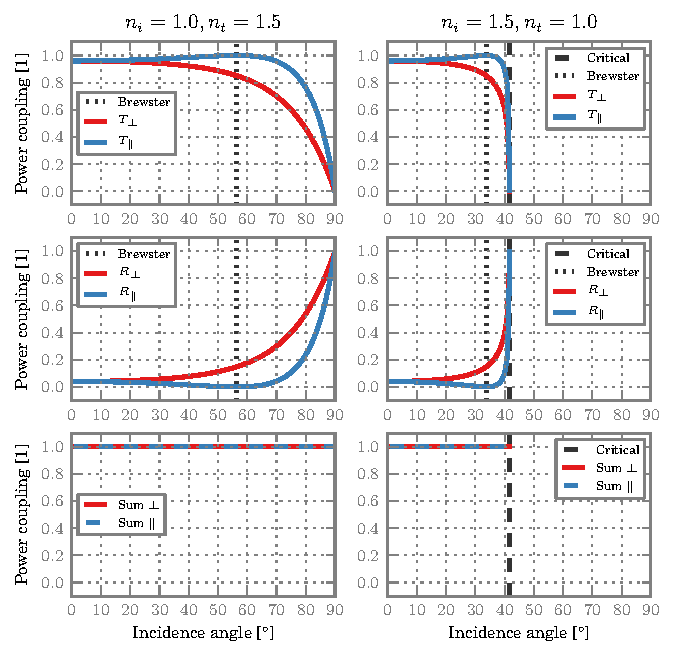
\includegraphics{interface_oblique_verification}
    \caption{Interface oblique, verification}
    \label{fig:interface_oblique_verification}
\end{figure}


%=============================================================================
\subsection{Thin film at normal incidence}
\label{sec:thin_film_at_normal_incidence}

%-----------------------------------------------------------------------------
\subsubsection{Scattering matrix}

Two interfaces separate three regions of space of refractive indices~$n_1$, $n_2$ and~$n_3$ (in most cases, $n_1=n_3$).
Each interface of the film reflects and transmits radiation according to the Fresnel equations for normal incidence~\eqref{eq:fresnel_normal}.
\Cref{fig:thin_film_normal} defines the notations for the reflection and transmission coeffients between the three regions of space.
The propagation between the two interfaces introduces a factor $a$.
\Cref{fig:thin_film_normal_collapsed} is what results of our modeling effort: a single network with two reflections and two transmissions.

\begin{figure}[hbtp]
    \centering
    \input{thin_film_normal.pdf_tex}
    \caption{Thin film at normal incidence.}
    \label{fig:thin_film_normal}
\end{figure}
\begin{figure}[hbtp]
    \centering
    \input{thin_film_normal_collapsed.pdf_tex}
    \caption{Thin film at normal incidence, collapsed.}
    \label{fig:thin_film_normal_collapsed}
\end{figure}

\Crefrange{eq:thin_film_normal_0}{eq:thin_film_normal_2} walk us through the derivation of~$r_{1, 3}$, the reflection coefficient of the thin film seen from the region of refractive index~$n_1$.
\begin{align}
    r_{1,3}
    &= r_{1,2} + t_{1,2}
        \left(
            a r_{2,3} a +
            a r_{2,3} a r_{2,1} a r_{2,3} a +
            \cdots
        \right)
       t_{2,1}
    \label{eq:thin_film_normal_0}
    \\
    r_{1, 3}
    &=
    r_{1, 2} + t_{1, 2} t_{2, 1} a^2r_{2, 3}
        \sum_{i=0}^{\infty} (a^2r_{2,1}r_{2,3})
    \label{eq:thin_film_normal_1}
    \\
    r_{1, 3}
    &=
    r_{1, 2} + t_{1, 2} t_{2, 1} a^2 r_{2, 3}
    \frac{1}{1 - a^2 r_{2, 1} r_{2, 3}}
    \label{eq:thin_film_normal_2}
\end{align}
Likewise, we can derive $r_{3, 1}$, $t_{1, 3}$ and $t_{3, 1}$.
They are given by \crefrange{eq:thin_film_normal_r31}{eq:thin_film_normal_t31},
with \cref{eq:thin_film_normal_r13} being a mere reminder of \cref{eq:thin_film_normal_2}.
\begin{subequations}
    \begin{align}
        r_{1, 3}
        &=
        r_{1, 2} + t_{1, 2} t_{2, 1} a^2 r_{2, 3}
        \frac{1}{1 - a^2 r_{2, 1} r_{2, 3}}
        \label{eq:thin_film_normal_r13}
        \\
        r_{3, 1}
        &=
        r_{3, 2} + t_{3, 2} t_{2, 3} a^2 r_{2, 1}
        \frac{1}{1 - a^2 r_{2, 3} r_{2, 1}}
        \label{eq:thin_film_normal_r31}
        \\
        t_{1, 3}
        &=
        t_{1,2} t_{2,3} a \frac{1}{1 - a^2 r_{2, 3} r_{2, 1}}
        \label{eq:thin_film_normal_t13}
        \\
        t_{3, 1}
        &=
        t_{3,2} t_{2,1} a \frac{1}{1 - a^2 r_{2, 1} r_{2, 3}}
        \label{eq:thin_film_normal_t31}
    \end{align}
\end{subequations}
The parameters $r_{1, 2}$, $t_{1, 2}$, $r_{3, 2}$, $t_{3, 2}$, $r_{2, 1}$, $t_{2, 1}$,
$r_{2, 3}$ and $t_{2, 3}$ are determined by the Fresnel equations for normal incidence~\eqref{eq:fresnel_normal}.
The parameter $a$ is determined by $\exp(-i 2 \pi d n f / c_0)$ according to \cref{eq:net_distance}.
Note that in these four equations, the fraction is the same;
it is sufficient to compute its value once only.



There is one more factor to apply: a compensation for the space taken by the film.
As illustrated in \cref{fig:thin_film_normal_compensation},
the film has a thickness $d_2$ and
its center is located at distances $d_1$ and $d_3$ from other reference points.
The actual length of the medium 1 is not $d_1$ but $d_1 - d_2/2$.
Likewise, the wave travels a distance $d_3 - d_2/2$ in the medium 3.
\begin{figure}[hbtp]
    \centering
    \input{thin_film_normal_compensation.pdf_tex}
    \caption{Thin film at normal incidence, space compensation.}
    \label{fig:thin_film_normal_compensation}
\end{figure}
One way of accounting for this without changing any other network is to add some negative space on each side of the film.
Let $a_1$ and $a_3$ be the effect of these negative spaces.
\Crefrange{eq:negative_space_3}{eq:negative_space_3} apply \cref{eq:net_distance} to the refractive indices $n_1$ and $n_3$ for the negative distance $-d_2/2$.
\begin{subequations}
    \begin{align}
        a_1 &= \exp \Big(-i 2 \pi (-d_2/2) n_1 f / c_0 \Big) \label{eq:negative_space_1}
        \\
        a_3 &= \exp \Big(-i 2 \pi (-d_2/2) n_3 f / c_0 \Big) \label{eq:negative_space_3}
    \end{align}
    \label{eq:negative_space}
\end{subequations}
The reflection on the left side crosses the negative space $a_1$ twice, therefore $r_{1, 3}$ must be multiplied by $a_1^2$.
Likewise, $r_{3, 1}$ must be multiplied by $a_3^2$.
Both transmissions $t_{1, 3}$ and $t_{3, 1}$ go through $a_1$ and $a_3$, therefore they must be multiplied by $a_1 a_3$.
This is summarized with \crefrange{eq:thin_film_normal_compensated_r13}{eq:thin_film_normal_compensated_t31}.
\begin{subequations}
    \begin{align}
        r'_{1, 3} &= a_1^2   \, r_{1, 3} \label{eq:thin_film_normal_compensated_r13} \\
        r'_{3, 1} &= a_3^2   \, r_{3, 1} \label{eq:thin_film_normal_compensated_r31} \\
        t'_{1, 3} &= a_1 a_3 \, t_{1, 3} \label{eq:thin_film_normal_compensated_t13} \\
        t'_{3, 1} &= a_1 a_3 \, t_{3, 1} \label{eq:thin_film_normal_compensated_t31}
    \end{align}
    \label{eq:thin_film_normal_compensated}
\end{subequations}

From there, building the scattering matrix of the thin film is straightforward.
If we name $I_3$ the 3--by--3 identity matrix,
then the Jones matrices  \crefrange{eq:thin_film_normal_s11}{eq:thin_film_normal_s22}
are the elements of the scattering matrix.
\begin{subequations}
    \begin{align}
        S_{1, 1} &= r'_{1, 3} I_3 \label{eq:thin_film_normal_s11} \\
        S_{1, 2} &= t'_{3, 1} I_3 \label{eq:thin_film_normal_s12} \\
        S_{2, 1} &= t'_{1, 3} I_3 \label{eq:thin_film_normal_s21} \\
        S_{2, 2} &= r'_{3, 1} I_3 \label{eq:thin_film_normal_s22}
    \end{align}
    \label{eq:thin_film_normal_sij}
\end{subequations}
If necessary, each of these Jones matrices can be adapted to account for the orientation of the thin film;
see~\vref{sec:rotating_jones_matrices}.

%-----------------------------------------------------------------------------
\subsubsection{Verification}
We have derived a model that treats a thin film as a single two-ports network.
It should yield the same results as a system of three networks
(interface--space--interface).
In this section, we verify this numerically.

\Cref{fig:thin_film_normal_verification_principle} defines the distances and refractive indices used in this section.
It also illustrates the two systems that we wish to compare:
\begin{itemize}
    \item one system made of three networks (two spaces, one thin film), that we call ``thin film model'';
    \item one system made of five networks (three spaces and two interfaces), that we call ``interfaces model''.
\end{itemize}
\begin{figure}[hbtp]
    \centering
    \input{thin_film_normal_verification_principle.pdf_tex}
    \caption{Thin film at normal incidence, verification, principle.}
    \label{fig:thin_film_normal_verification_principle}
\end{figure}

\Cref{fig:thin_film_normal_verification} presents the result of both models for
$n_1=1.00$, $n_2=1.75$, $n_3=1.50$,
$d_1=\SI{1}{\meter}$, $d_2=\SI{10}{\micro\meter}$ and $d_3=\SI{1}{\meter}$.
The source is on the leftmost port.
The ``Reflected'' plot corresponds to the output of that leftmost port.
The ``Transmitted'' plot corresponds to the output of the rightmost port.
\begin{figure}[hbtp]
    \centering
    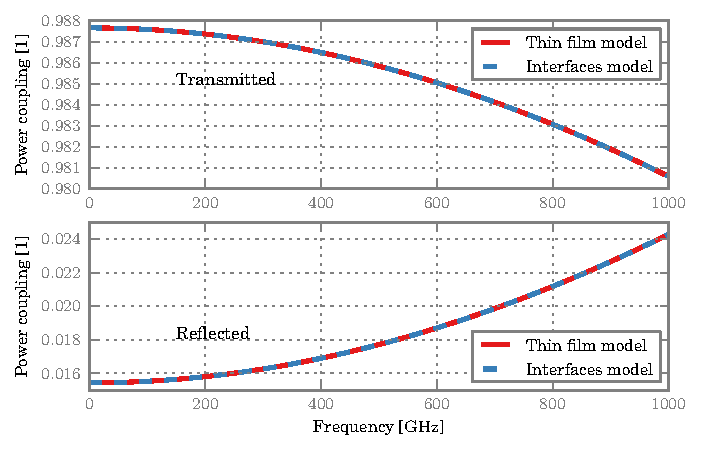
\includegraphics{thin_film_normal_verification.pdf}
    \caption{Thin film at normal incidence, verification.}
    \label{fig:thin_film_normal_verification}
\end{figure}

Both models agree within numerical noise.
The advantage of the thin film model over the other is that a thin film is represented by a single network.
This is easier for the programmer and faster for the computer.

The curvature of the power coupling displayed in \cref{fig:thin_film_normal_verification} comes from standing waves inside the thin film.
\Cref{eq:cavity_period} predicts a period of $F = c_0 / (2 n_2 d_2) \approx \SI{9993}{\tera\hertz}$.
Thin cavities (here \SI{10}{\micro\meter}) create standing wave patterns with very large periods.



%=============================================================================
\subsection{Thin film at oblique incidence}
\label{sec:thin_film_at_oblique_incidence}

A thin film at oblique incidence forms a four-ports network.
\Cref{fig:thin_film_oblique} defines the geometry and the port-numbering that we use.
\begin{figure}[hbtp]
    \centering
    \missingfigure{Thin film oblique}
    \caption{Thin film at oblique incidence}
    \label{fig:thin_film_oblique}
\end{figure}

When deriving the scattering matrix of a thin film at normal incidence in \cref{sec:thin_film_at_normal_incidence}, we allowed for three refractive indices: one for the film itself and one for each propagation medium on each side of the film.
This was a generalization that came at barely no cost because the geometry was simple.
In the case of a thin film at oblique incidence, we assume that the propagation medium on each side of the thin film has the same refractive index.
This is, after all, the most common case;
for example, a beam splitter placed in vacuum has vacuum on both sides.
If that constraint is too strong, it is always possible to model that thin film with three networks by using two interfaces and a distance (see sections~\ref{sec:generic_networks_distance} and \ref{sec:interface_at_oblique_incidence}).

%-----------------------------------------------------------------------------
\subsubsection{Geometry}
\label{sec:thin_film_geometry}
We need to determine the angle of incidence, the parallel and perpendicular decomposition matrices and the various rotation matrices.

It is assumed that we know the orientation of the thin film via its normal $n$ and the direction of propagation $k_1$ of the wave incident to the port 1.

From $n$ and $k_1$, we can apply \cref{eq:angle_from_dot_product} to compute the angle of incidence~$\theta_a$.
We get the refracted angle~$\theta_b$ from $\theta_a$ with \cref{eq:snell_thetab}.

We use \cref{eq:normal_to_plane_of_incidence} to retreive the normal to the plane of incidence $u$.

From the normal $u$ to the plane of incidence
and \cref{eq:para_perp_decomposition_matrix},
we determine the parallel and perpendicular projection matrices,
$M_\parallel$ and $M_\perp$.

From $u$ and
equations~\eqref{eq:quaternion_rotation_around_axis}
and \eqref{eq:quaternion_to_rotation_matrix}, we can compute the rotation matrices to apply to the Jones matrices and the direction of propagation.
The angles that we need are listed in \cref{eq:thin_film_angles}.
\begin{equation}
    \begin{aligned}
        \theta_{1 \leftarrow 2} &= 2 \theta_a
        &
        \theta_{2 \leftarrow 1} &= -2 \theta_a
        \\
        \theta_{3 \leftarrow 4} &= 2 \theta_a
        &
        \theta_{4 \leftarrow 3} &= -2 \theta_a
        \\
        \theta_{4 \leftarrow 1} &= -2 \theta_a
    \end{aligned}
    \label{eq:thin_film_angles}
\end{equation}
These angles $\theta_{i \leftarrow j}$ have corresponding rotation matrices $R^{i \leftarrow j}$.
We can already determine the directions of propagation of the waves exiting the thin film with \cref{eq:thin_film_propagation_rotation_ki}.
\begin{subequations}
    \begin{align}
        k_2 &= -R^{2 \leftarrow 1} k_1
        \label{eq:thin_film_propagation_rotation_k2}\\
        k_3 &= k_1
        \label{eq:thin_film_propagation_rotation_k3}\\
        k_4 &= R^{4 \leftarrow 1} k_1
        \label{eq:thin_film_propagation_rotation_k4}
    \end{align}
    \label{eq:thin_film_propagation_rotation_ki}
\end{subequations}

%-----------------------------------------------------------------------------
\subsubsection{Reflection and transmission coefficients}
In the previous section (\cref{sec:thin_film_geometry}) we have determined the decomposition and rotation matrices that are needed to compute the reflection and refraction coefficients of a thin film at oblique incidence.
We also have the angle of incidence and the refracted angle.

We want to apply the Fresnel equations for oblique incidence \eqref{eq:fresnel_oblique} twice:
once for entering the thin film, and once for leaving it.
\begin{itemize}
    \item 
$r_{\parallel a}$, $r_{\perp a}$, $t_{\parallel a}$ and $t_{\perp a}$ correspond to entering the film.
They are derived from \cref{eq:fresnel_oblique} with
$\theta_i = \theta_a$, $\theta_t = \theta_b$,
$n_i = n_a$ and $n_t = n_b$.
    \item
$r_{\parallel b}$, $r_{\perp b}$, $t_{\parallel b}$ and $t_{\perp b}$ correspond to exiting the film.
They are derived from \cref{eq:fresnel_oblique} with
$\theta_i = \theta_b$, $\theta_t = \theta_a$,
$n_i = n_b$ and $n_t = n_a$.
\end{itemize}

The pathlength $l_b$ inside the film is not equal to the thickness $d$ of the thin film because $\theta_b \ne 0$, as described by \cref{eq:thin_film_oblique_pathlength}.
\begin{equation}
    l_b = \frac{d}{\cos \theta_b}
    \label{eq:thin_film_oblique_pathlength}
\end{equation}
To this distance $l_b$ corresponds a gain $a_b$ that we derive from \cref{eq:net_distance}.
Its expression is given for $l_b$ in \cref{eq:thin_film_distance}.
\begin{equation}
    a_b = \exp(-2i \pi l_b n_b f / c_0)
    \label{eq:thin_film_distance}
\end{equation}
This pathlength $l_b$ must be compensated for.
Indeed, the pathlength $l_b$ inside the film replaces a pathlength $l_a$ in the material $n_a$.
\begin{equation}
    l_a = \frac{d}{\cos \theta_a}
    \label{eq:thin_film_oblique_pathlength_compensation}
\end{equation}
\begin{equation}
    a_a = \exp(-2i \pi (-l_a) n_a f / c_0)
    \label{eq:thin_film_distance_compensation}
\end{equation}

What follows is similar to what we did for the thin film at normal incidence.
One difference is that do it twice, one for the parallel parameters and one for the perpendicular parameters.
Another difference is that we have two and not three refractive indices, which gives a few simplifications.
\begin{subequations}
    \begin{align}
        t_\parallel
        &=
        a_a \,
        t_{\parallel a} \, t_{\parallel b} \, a_b
        \frac{1}{
            1 - (r_{\parallel b} \, a_b)^2
        }
        \\
        t_\perp
        &=
        a_a \,
        t_{\perp a} \, t_{\perp b} \, a_b
        \frac{1}{
            1 - (r_{\perp b} \, a_b)^2
        }
        \\
        r_\parallel
        &=
        a_a \,
        r_{\parallel a} + r_{\parallel b} \, a_b \, t_\parallel
        \\
        r_\perp
        &=
        a_a \,
        r_{\perp a} + r_{\perp b} \, a_b \, t_\perp
    \end{align}
\end{subequations}

\subsubsection{Scattering matrix}
Because we use one refractive index only outside the film, the transmitted waves are not rotated.
\begin{equation}
    S_{1, 3} =
    S_{2, 4} =
    S_{3, 1} =
    S_{4, 2} =
    t_\parallel M_\parallel
    +
    t_\perp M_\perp
    \label{eq:thin_film_s_t}
\end{equation}

The reflections, however, require some rotations.
\begin{subequations}
    \begin{align}
        S_{1, 2} = R^{1 \leftarrow 2} (r_\parallel M_\parallel + r_\perp M_\perp) \\
        S_{2, 1} = R^{2 \leftarrow 1} (r_\parallel M_\parallel + r_\perp M_\perp) \\
        S_{3, 4} = R^{3 \leftarrow 4} (r_\parallel M_\parallel + r_\perp M_\perp) \\
        S_{4, 3} = R^{4 \leftarrow 3} (r_\parallel M_\parallel + r_\perp M_\perp)
    \end{align}
    \label{eq:thin_film_s_r}
\end{subequations}

Finally, many paths are forbidden.
\begin{equation}
    S_{1, 1} = S_{1, 4} = S_{2, 2} = S_{2, 3} =
    S_{3, 2} = S_{3, 3} = S_{4, 1} = S_{4, 4} = 
    \begin{pmatrix}
        0&0&0\\0&0&0\\0&0&0
    \end{pmatrix}
    \label{eq:thin_film_s_zero}
\end{equation}

\Crefrange{eq:thin_film_s_t}{eq:thin_film_s_zero} define the scattering parameters of the 4--by--4 scattering matrix of a thin film at oblique incidence.


\subsubsection{Verification}
Our model for a thin film at oblique incidence should provide exactly the same result as two interfaces and a distance.
The goal of the thin film model is to provide convenience, not introduce new physics.
\Cref{fig:thin_film_oblique_verification} illustrates a comparison between these two ways of modeling a thin film.
The angle of incidence is~\SI{45}{\degree}.
The film is~\SI{10}{\micro\meter} thick.
The refractive indices are 1.0 outside the film and 1.5 in the film.
The thickness of the film creates a cavity and therefore a standing wave.
This standing wave is responsable for the frequency-dependance of the reflected and transmitted power seen on \cref{fig:thin_film_oblique_verification}.

\begin{figure}[hbtp]
    \centering
    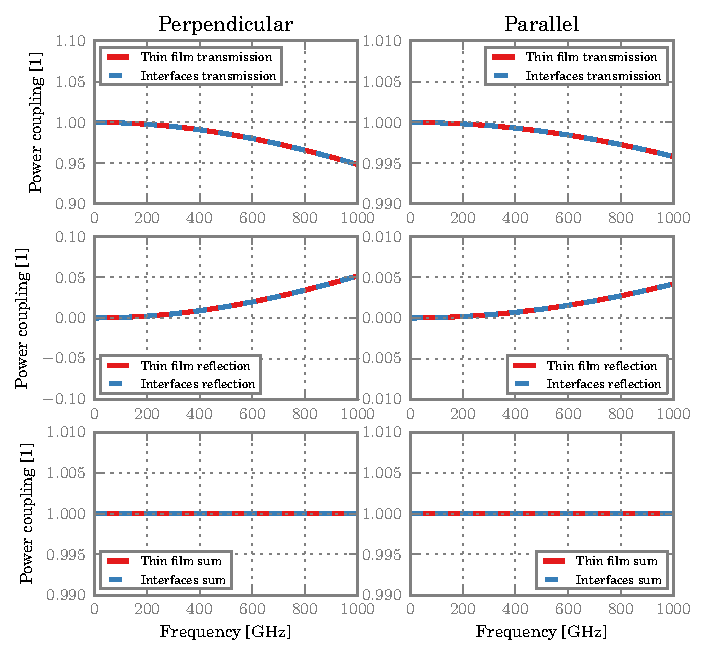
\includegraphics{thin_film_oblique_verification}
    \caption{Thin film oblique, verification}
    \label{fig:thin_film_oblique_verification}
\end{figure}

The top row of \cref{fig:thin_film_oblique_verification} shows the transmitted power, the middle row shows the reflected power, and the bottom row shows the sum of the two.
That last row shows that energy is conserved: the power that is not transmitted is reflected.

The left column shows the transmitted, reflected and total power coupling for the perpendicular polarization.
The right column corresponds to the parallel polarization.
Note that the vertical-axes differ for the two polarizations: the standing wave has an effect about ten times stronger on the perpendicular polarization.

Finally, each plot shows two overlapped curves.
The red curve corresponds to the model derived in this section with which the thin film is seen as a single network.
The blue curve corresponds to a model made of two interfaces and a distance.

As expected, both models agree within numerical noise.
This agreement does not only happen in power, but also in field.
The phasor predicted by both methods agree within $10^{-10}$: the magnitude of the difference of the phasors is smaller than $10^{-10}$ for frequencies of the order of \SI{1}{\tera\hertz}.  \todo{Should I put a pic?}



%=============================================================================
\subsection{Wire grid polarizer}
\todo{Check k omega convention}
In their paper from \citeyear{houde_2001} \citetitle{houde_2001}, \textcite{houde_2001} present a set of equations that approximate the electric field at any point near a wire grid polarizer.
The incident wave is assumed plane, the surrounding propagation medium is assumed homogeneous and isotropic, and the wires are assumed to be free floating (no dielectric substrate) and to have a cylindrical section.

\subsubsection{Geometry}
The article of \citeauthor{houde_2001} \cite{houde_2001} defines the following rest reference frame for the grid: wires in the $\vect{x}\vect{y}$ plane, wires along $\vect{x}$.
Its normal, at rest, is therefore the $\vect{z}$ axis.

If $R$ is the rotation matrix that move the grid from its rest attitude to its useful attitude, then the normal of the grid is $\vect{n}=R \vect{z}$.

The grid is a four port network.
$\vect{k}_1$,  is the direction of propagation of the wave indident to the port 1.
We can derive the direction of propagation of the wave incident to the three other ports easily.
The law of reflection states that $\vect{k}_1$, $\vect{k}_2$ and $\vect{n}$ are coplanar and that the directed angle between $\vect{k}_1$ and $\vect{n}$ equals that between $\vect{n}$ and $\vect{k}_2$.
Therefore, one way of deriving $\vect{k}_2$ is to rotate $\vect{k}_1$ by \SI{180}{\degree} around $\vect{n}$.
Then, $\vect{k}_3=-\vect{k}_1$ and $\vect{k}_4=-\vect{k_2}$.

\subsubsection{Reflection and transmission coefficients}
The set of equations that interest us here are the equations numbered 23 to 35, 62 and 63 in the article of \citeauthor{houde_2001} \cite{houde_2001}, which we copied here for convenience.
The first two equations, \eqref{eq:grid_current_linear} and \eqref{eq:grid_current_circular}, describe the electric current in the wires.
$K^x$ corresponds to a linear current and $K^\theta$ to a circular current.
In the first case, electrons move along the length of the wire; in the other, they rotate around the axis of the wire.
\begin{align}
    K^x &= \frac{E_0}{F} \cdot \alpha' \frac{N_x}{\Delta_x}
    \label{eq:grid_current_linear}
    \\
    K^\theta &= (-j) \frac{E_0}{F} \cdot (\gamma' \beta - \beta' \gamma) \frac{N_\theta}{\Delta_\theta}
    \label{eq:grid_current_circular}
\end{align}
with
\begin{align}
    N_x
    &=
    1 - j \frac{Z_s}{Z_0} \frac{ka}{2}
    \\
    \Delta_x
    &=
    (1 - \alpha^2) S_1 - j \frac{Z_s}{Z_0} \sqrt{1 - \alpha^2}H_1^{(2)} (k'a)
    \\
    N_\theta
    &=
    1 + j \frac{Z_s}{Z_0} \frac{2}{ka}
    \\
    \Delta_\theta
    &=
    \sqrt{1 - \alpha^2} H_1^{(2)} (k'a) + j \frac{Z_s}{Z_0} (1 - \alpha^2) S_1
\end{align}
and
\begin{equation}
    S_1 = H_0^{(2)} (k'a) + 2
    \sum_{n=1}^\infty
    H_0^{(2)}(k'nd) \cos (k \beta nd)
    \text{.}
    \label{eq:infinite_hankel}
\end{equation}
The following equations use the previous definitions.
They describe the reflected and transmitted fields in three dimensions for a grid in the $xy$-plane, wires along~$x$.
\begin{align}
    R^x
    &=
    -\frac{F}{E_0}
    \frac{\lambda}{\pi d}
    \frac{1 - \alpha^2}{\gamma} K^x
    \label{eq:houde_Rx}
    \\
    R^y
    &=
    \phantom{-}
    \frac{F}{E_0}
    \frac{\lambda}{\pi d}
    \left[
        \frac{\alpha \beta}{\gamma} K^x
        -
        j \frac{ka}{2} K^\theta
    \right]
    \\
    R^z
    &=
    -\frac{F}{E_0}
    \frac{\lambda}{\pi d}
    \left[
       \alpha K^x
       +
       j \frac{\beta}{\gamma} \frac{ka}{2} K^\theta
    \right]
    \\
    T^x &= \alpha' + R^x
    \\
    T^y
    &=
    \beta' +
    \frac{F}{E_0}
    \frac{\lambda}{\pi d}
    \left[
        \frac{\alpha \beta}{\gamma} K^x + j \frac{ka}{2} K^\theta
    \right]
    \\
    T^z
    &=
    \gamma' +
    \frac{F}{E_0}
    \frac{\lambda}{\pi d}
    \left[
        \alpha K^x - j \frac{\beta}{\gamma} \frac{ka}{2} K^\theta
    \right]
\end{align}
Note that Houde calls these $R$ and $T$ ``reflection'' and ``transmission coefficient'', something they are not quite since they contain $\alpha'$, $\beta'$ and $\gamma'$, corresponding to the amplitude of the incoming electric field in the three dimensions.
These amplitudes have to be factored out if we want to really speak about reflection or transmission coefficients.

When implementing these equations, some simplifications are obvious.
For example, $\frac{E_0}{F}$ inside $K^x$ and $K^\theta$ cancels $\frac{F}{E_0}$ in $R$ and $T$;
the complex unit $j$ within $K^\theta$ combines with $j$ in $R$ and $T$ to become -1.

In these equations, $\alpha'$, $\beta'$ and $\gamma'$ are the three components of the direction of the incident electric field, satisfying $\alpha'^2 + \beta'^2 + \gamma'^2 = 1$.
That condition seems to apply only to real numbers, restricting the use of this grid model to waves that are linearly polarized (their three components are in phase).
However, there is no such limitation in the model.
Indeed, the authors define the incident electric field as $(e_x, e_y, e_z) = E_0(\alpha', \beta', \gamma')$.
The amplitude $E_0$ can be complex and it seems that its phase has to be shared among the three components.
However, when we rewrite the equations to fit in a matrix, we will notice that the real parameters are not $\alpha'$, $\beta'$, $\gamma'$ and $E_0$, but $e_x$, $e_y$ and $e_z$ directly, which are all independant.
In that case, each of them is free to have its own phase and the model also applies to elliptically polarized waves.


In order to rewrite these equations in a matrix form that depends on $e_x$, $e_y$ and $e_z$, one needs to split each coefficient of transmission and reflection into three, like this:
\begin{equation}
    e_{rx} = R^{xx} e_x + R^{xy} e_y + R^{xz} e_z
\end{equation}
so that we can write
\begin{align}
    e_r &= R e_i \\
    e_r &=
    \begin{pmatrix}
        R_{xx} & R_{xy} & R_{xz} \\
        R_{yx} & R_{yy} & R_{yz} \\
        R_{zx} & R_{zy} & R_{zz}
    \end{pmatrix}
    e_i
\end{align}
for the reflection $R$ and a similar equation for the transmission $e_t = T e_i$.
I start with $R_x$ defined in \cref{eq:houde_Rx} to get $R_{xx}$, $R_{xy}$ and $R_{xz}$.
\begin{align*}
    e_{rx} &= R^x E_0
    \\
           &= -\frac{F}{E_0}
              \frac{\lambda}{\pi d}
              \frac{1-\alpha^2}{\gamma}
              K^x
              E_0
    \\
           &= -\cancel{\frac{F}{E_0}}
              \frac{\lambda}{\pi d}
              \frac{1-\alpha^2}{\gamma}
              \cancel{\frac{E_0}{F}}
              \frac{N_x}{\Delta_x}
              \underbrace{
                  \alpha'
                  E_0
              }_{e_{ix}}
    \\
           &= -\frac{\lambda}{\pi d}
              \frac{1-\alpha^2}{\gamma}
              \frac{N_x}{\Delta_x}
              e_{ix}
\end{align*}
By identification, we find these values for $R_{xx}$, $R_{xy}$ and $R_{xz}$.
\begin{equation}
    \left\lbrace
    \begin{aligned}
        R_{xx} &= -\frac{\lambda}{\pi d}
                  \frac{N_x}{\Delta_x}
                  \frac{1-\alpha^2}{\gamma}
        \\
        R_{xy} &= 0
        \\
        R_{xz} &= 0
    \end{aligned}
    \right.
\end{equation}
Let us continue with $R_y$.
\begin{align*}
    e_{ry}
    &= R^y E_0
    \\
    &= \frac{F}{E_0}
       \frac{\lambda}{\pi d}
       \left[
           \frac{\alpha \beta}{\gamma}
           K^x
           -
           j
           \frac{ka}{2}
           K^\theta           
       \right]
       E_0
    \\
    &= \cancel{\frac{F}{E_0}}
       \frac{\lambda}{\pi d}
       \left[
           \frac{\alpha \beta}{\gamma}
           \cancel{\frac{E_0}{F}}
           \frac{N_x}{\Delta_x}
           \alpha'
           -
           j
           \frac{ka}{2}
           (-j)
           \cancel{\frac{E_0}{F}}
           \frac{N_\theta}{\Delta_\theta}
           (\gamma' \beta - \beta' \gamma)           
       \right]
       E_0
    \\
    &= \frac{\lambda}{\pi d}
       \left[
           \frac{\alpha \beta}{\gamma}
           \frac{N_x}{\Delta_x}
           \alpha'
           +
           \frac{ka}{2}
           \frac{N_\theta}{\Delta_\theta}
           \gamma
           \beta'
           -
           \frac{ka}{2}
           \frac{N_\theta}{\Delta_\theta}
           \beta
           \gamma'
       \right]
       E_0
    \\
    &= \frac{\lambda}{\pi d}
       \frac{\alpha \beta}{\gamma}
       \frac{N_x}{\Delta_x}
       \underbrace{E_0 \alpha'}_{e_{ix}}
       +
       \frac{\lambda}{\pi d}
       \frac{ka}{2}
       \frac{N_\theta}{\Delta_\theta}
       \gamma
       \underbrace{E_0 \beta'}_{e_{iy}}
       -
       \frac{\lambda}{\pi d}
       \frac{ka}{2}
       \frac{N_\theta}{\Delta_\theta}
       \beta
       \underbrace{E_0 \gamma'}_{e_{iz}}
\end{align*}
\begin{equation}
    \left\lbrace
    \begin{aligned}
        R_{yx}
        &=
        \phantom{-}
        \frac{\lambda}{\pi d}
        \frac{N_x}{\Delta_x}
        \frac{\alpha \beta}{\gamma}
        \\
        R_{yy}
        &=
        \phantom{-}
        \frac{\lambda}{\pi d}
        \frac{N_\theta}{\Delta_\theta}
        \frac{ka}{2}
        \gamma
        \\
        R_{yz}
        &=
        -
        \frac{\lambda}{\pi d}
        \frac{N_\theta}{\Delta_\theta}
        \frac{ka}{2}
        \beta
    \end{aligned}
    \right.
\end{equation}
Same thing for $R_z$.
\begin{align*}
    e_{rz} &= R^z E_0
    \\
    &=
    -
    \frac{F}{E_0}
    \frac{\lambda}{\pi d}
    \left[
        \alpha K^x
        +
        j
        \frac{\beta}{\gamma}
        \frac{ka}{2}
        k^\theta
    \right]
    E_0
    \\
    &=
    -
    \cancel{\frac{F}{E_0}}
    \frac{\lambda}{\pi d}
    \left[
        \alpha
        \cancel{\frac{E_0}{F}}
        \frac{N_x}{\Delta_x}
        \alpha'
        +
        j
        \frac{\beta}{\gamma}
        \frac{ka}{2}
        (-j)
        \cancel{\frac{E_0}{F}}
        (\gamma' \beta - \beta' \gamma)
        \frac{N_\theta}{\Delta_\theta}
    \right]
    E_0
    \\
    &=
    -
    \frac{\lambda}{\pi d}
    \alpha
    \frac{N_x}{\Delta_x}
    \underbrace{E_0 \alpha'}_{e_{ix}}
    +
    \frac{\lambda}{\pi d}
    \frac{\beta}{\gamma}
    \frac{ka}{2}
    \frac{N_\theta}{\Delta_\theta}
    \gamma
    \underbrace{E_0 \beta'}_{e_{iy}}
    -
    \frac{\lambda}{\pi d}
    \frac{\beta}{\gamma}
    \frac{ka}{2}
    \frac{N_\theta}{\Delta_\theta}
    \beta
    \underbrace{E_0 \gamma'}_{e_{iz}}
\end{align*}
\begin{equation}
    \left\lbrace
    \begin{aligned}
        R_{zx}
        &=
        -
        \frac{\lambda}{\pi d}
        \frac{N_x}{\Delta_x}
        \alpha
        \\
        R_{zy}
        &=
        \phantom{-}
        \frac{\lambda}{\pi d}
        \frac{N_\theta}{\Delta_\theta}
        \frac{ka}{2}
        \beta
        \\
        R_{zz}
        &=
        -
        \frac{\lambda}{\pi d}
        \frac{N_\theta}{\Delta_\theta}
        \frac{ka}{2}
        \frac{\beta^2}{\gamma}
    \end{aligned}
    \right.
\end{equation}
We have the reflection matrix.
Now, we compute the transmission matrix.
\begin{align*}
    e_{tx} &= T^x E_0
    \\
    &= (\alpha' + R^x) E_0
    \\
    &= \underbrace{\alpha' E_0}_{e_{ix}}
       -
       \frac{\lambda}{\pi d}
       \frac{1 - \alpha^2}{\gamma}
       \frac{N_x}{\Delta_x}
       \underbrace{\alpha' E_0}_{e_{ix}}
    \\
    &= \left(
           1
           -
           \frac{\lambda}{\pi d}
           \frac{1 - \alpha^2}{\gamma}
           \frac{N_x}{\Delta_x}
       \right)
       e_{ix}
\end{align*}
\begin{equation}
    \left\lbrace
    \begin{aligned}
        T_{xx}
        &= 1
           -
           \frac{\lambda}{\pi d}
           \frac{N_x}{\Delta_x}
           \frac{1 - \alpha^2}{\gamma}
        \\
        T_{xy} &= 0
        \\
        T_{xz} &= 0
    \end{aligned}
    \right.
\end{equation}

\begin{align*}
    e_{ty} &= T^y E_0
    \\
    &=
    \left(
        \beta'
        +
        \frac{F}{E_0}
        \frac{\lambda}{\pi d}
        \left[
            \frac{\alpha \beta}{\gamma}
            K^x
            +
            j
            \frac{ka}{2}
            K^\theta
        \right]
    \right)
    E_0
    \\
    &=
    \left(
        \beta'
        +
        \cancel{\frac{F}{E_0}}
        \frac{\lambda}{\pi d}
        \left[
            \frac{\alpha \beta}{\gamma}
            \cancel{\frac{E_0}{F}}
            \frac{N_x}{\Delta_x}
            \alpha'
            +
            j
            \frac{ka}{2}
            (-j)
            \cancel{\frac{E_0}{F}}
            \frac{N_\theta}{\Delta_\theta}
            (\gamma' \beta - \beta' \gamma)
        \right]
    \right)
    E_0
    \\
    &=
    \left(
        \beta'
        +
        \frac{\lambda}{\pi d}
        \frac{\alpha \beta}{\gamma}
        \frac{N_x}{\Delta_x}
        \alpha'
        -
        \frac{\lambda}{\pi d}
        \frac{ka}{2}
        \frac{N_\theta}{\Delta_\theta}
        \gamma
        \beta'
        +
        \frac{\lambda}{\pi d}
        \frac{ka}{2}
        \frac{N_\theta}{\Delta_\theta}
        \beta
        \gamma'
    \right)
    E_0
    \\
    &=
    \frac{\lambda}{\pi d}
    \frac{\alpha \beta}{\gamma}
    \frac{N_x}{\Delta_x}
    \underbrace{E_0 \alpha'}_{e_{ix}}
    +
    \left(
        1
        -
        \frac{\lambda}{\pi d}
        \frac{ka}{2}
        \frac{N_\theta}{\Delta_\theta}
        \gamma
    \right)
    \underbrace{E_0 \beta'}_{e_{iy}}
    +
    \frac{\lambda}{\pi d}
    \frac{ka}{2}
    \frac{N_\theta}{\Delta_\theta}
    \beta
    \underbrace{E_0 \gamma'}_{e_{iz}}
\end{align*}
\begin{equation}
    \left\lbrace
    \begin{aligned}
        T_{yx}
        &= \frac{\lambda}{\pi d}
           \frac{N_x}{\Delta_x}
           \frac{\alpha \beta}{\gamma}
        \\
        T_{yy}
        &= 1
           -
           \frac{\lambda}{\pi d}
           \frac{N_\theta}{\Delta_\theta}
           \frac{ka}{2}
           \gamma
        \\
        T_{yz}
        &= \frac{\lambda}{\pi d}
           \frac{N_\theta}{\Delta_\theta}
           \frac{ka}{2}
           \beta
    \end{aligned}
    \right.
\end{equation}

\begin{align*}
    e_{tz} &= T^z E_0
    \\
    &=
    \left(
        \gamma' +
        \frac{F}{E_0}
        \frac{\lambda}{\pi d}
        \left[
            \alpha K^x - j \frac{\beta}{\gamma} \frac{ka}{2} K^\theta
        \right]
    \right)
    E_0
    \\
    &=
    \left(
        \gamma' +
        \cancel{\frac{F}{E_0}}
        \frac{\lambda}{\pi d}
        \left[
            \alpha
            \cancel{\frac{E_0}{F_0}}
            \frac{N_x}{\Delta_x}
            \alpha'
            -
            j
            \frac{\beta}{\gamma}
            \frac{ka}{2}
            (-j)
            \cancel{\frac{E_0}{F}}
            \frac{N_\theta}{\Delta_\theta}
            (\gamma' \beta - \beta' \gamma)
        \right]
    \right)
    E_0
    \\
    &=
    \left(
        \gamma' +
        \frac{\lambda}{\pi d}
        \left[
            \alpha
            \frac{N_x}{\Delta_x}
            \alpha'
            +
            \frac{\beta}{\gamma}
            \frac{ka}{2}
            \frac{N_\theta}{\Delta_\theta}
            \gamma
            \beta'
            -
            \frac{\beta}{\gamma}
            \frac{ka}{2}
            \frac{N_\theta}{\Delta_\theta}
            \beta
            \gamma'
        \right]
    \right)
    E_0
    \\
    &=
    \frac{\lambda}{\pi d}
    \alpha
    \frac{N_x}{\Delta_x}
    \underbrace{E_0 \alpha'}_{e_{ix}}
    +
    \frac{\lambda}{\pi d}
    \frac{\beta}{\gamma}
    \frac{ka}{2}
    \frac{N_\theta}{\Delta_\theta}
    \gamma
    \underbrace{E_0 \beta'}_{e_{iy}}
    +
    \left(
        1
        -
        \frac{\lambda}{\pi d}
        \frac{\beta}{\gamma}
        \frac{ka}{2}
        \frac{N_\theta}{\Delta_\theta}
        \beta
    \right)
    \underbrace{E_0 \gamma'}_{e_{iz}}
\end{align*}
\begin{equation}
    \left\lbrace
    \begin{aligned}
        T_{zx}
        &= \frac{\lambda}{\pi d}
           \frac{N_x}{\Delta_x}
           \alpha
        \\
        T_{zy}
        &= \frac{\lambda}{\pi d}
           \frac{N_\theta}{\Delta_\theta}
           \frac{ka}{2}
           \frac{\beta}{\gamma}
           \gamma
        \\
        T_{zz}
        &= 1
           -
           \frac{\lambda}{\pi d}
           \frac{N_\theta}{\Delta_\theta}
           \frac{ka}{2}
           \frac{\beta}{\gamma}
           \beta
    \end{aligned}
    \right.
\end{equation}

Another simplification:
\begin{equation}
    k = 2\pi / \lambda
    \quad \Rightarrow \quad
    \frac{\lambda}{\pi d} \frac{ka}{2}
    =
    \frac{\lambda}{\pi d} \frac{2\pi a}{2\lambda}
    =
    \frac{a}{d}
\end{equation}

\begin{equation}
    R =
    \begin{pmatrix}
        -\frac{\lambda}{\pi d}
        \frac{N_x}{\Delta_x}
        \frac{1 - \alpha^2}{\gamma}
        &
        0
        &
        0
        \\
        \frac{\lambda}{\pi d}
        \frac{N_x}{\Delta_x}
        \frac{\alpha \beta}{\gamma}
        &
        \frac{\lambda}{\pi d}
        \frac{N_\theta}{\Delta_\theta}
        \frac{ka}{2}
        \gamma
        &
        -
        \frac{a}{d}
        \frac{N_\theta}{\Delta_\theta}
        \beta
        \\
        -
        \frac{\lambda}{\pi d}
        \frac{N_x}{\Delta_x}
        \alpha
        &
        \frac{a}{d}
        \frac{N_\theta}{\Delta_\theta}
        \beta
        &
        -
        \frac{a}{d}
        \frac{N_\theta}{\Delta_\theta}
        \frac{\beta^2}{\gamma}
    \end{pmatrix}
\end{equation}
\begin{equation}
    T =
    \begin{pmatrix}
        1 -
        \frac{\lambda}{\pi d}
        \frac{N_x}{\Delta_x}
        \frac{1 - \alpha^2}{\gamma}
        &
        0
        &
        0
        \\
        \frac{\lambda}{\pi d}
        \frac{N_x}{\Delta_x}
        \frac{\alpha \beta}{\gamma}
        &
        1 -
        \frac{a}{d}
        \frac{N_\theta}{\Delta_\theta}
        \gamma
        &
        \frac{a}{d}
        \frac{N_\theta}{\Delta_\theta}
        \beta
        \\
        \frac{\lambda}{\pi d}
        \frac{N_x}{\Delta_x}
        \alpha
        &
        \frac{a}{d}
        \frac{N_\theta}{\Delta_\theta}
        \beta
        &
        1 -
        \frac{a}{d}
        \frac{N_\theta}{\Delta_\theta}
        \frac{\beta^2}{\gamma}
    \end{pmatrix}
\end{equation}
These reflection and transmission matrices are Jones matrices.
The parameters are the radius $a$ of the wires,
the distance $d$ between the wires,
the conductivity $\sigma$ of the wires,
the frequency $f$ of the wave and
the direction of propagation $\vect{k_1}=(\alpha, \beta, \gamma)$.
We could consider the impedance of the surrounding medium as an additional parameter instead of using that of vacuum, but we did not need that.

\subsubsection{Scattering matrices}
The reflection and transmission matrices defined above are Jones matrices.
But before, we must apply rotation matrices to them in order to account for the arbitrary orientation of the grid.
Indeed, these Jones matrices are valid for grid lying in the $(x, y)$ plane, with the wires along $x$.






%#############################################################################

\section{Simple systems}
\label{sec:simple_systems}

The idea is to show that it works and makes sense.



%=============================================================================

\subsection{The simplest cavity}
\label{sec:the_simplest_cavity}

\Cref{fig:simple_cavity_principle} illustrates how three networks can represent a simple cavity: two interfaces separated by some space.
The three networks all have two ports numbered according to \cref{fig:simple_cavity_principle}.
Ports 2 and 3 are coupled, and so are ports 4 and 5.
Ports 1 and 6 are open to the outside world.

\begin{figure}[hbtp]
    \centering
    \input{simple_cavity_principle.pdf_tex}
    \caption{Simple cavity, principle.}
    \caption*{
        Two reflective surfaces facing each other form a cavity.
        Here, the surfaces are defined by the interfaces (vertical dotted lines)
        between regions of space of different refractive indices $n_1$ and $n_2$.
        According to the Fresnel equations~\eqref{eq:fresnel_normal}, these interfaces
        reflect and transmit part of the incident radiation (black arrows).
        As a result, a standing wave is formed inside the cavity.
        That standing wave is the superposition of an infinity of traveling waves
        interfering with each other.
        We can model such a system with three two-ports networks:
        one for each interface and one for the space between them.
        The numbers 1 to~6 are our arbitrary labels for the ports.
    }
    \label{fig:simple_cavity_principle}
\end{figure}
\begin{figure}[hbtp]
    \centering
    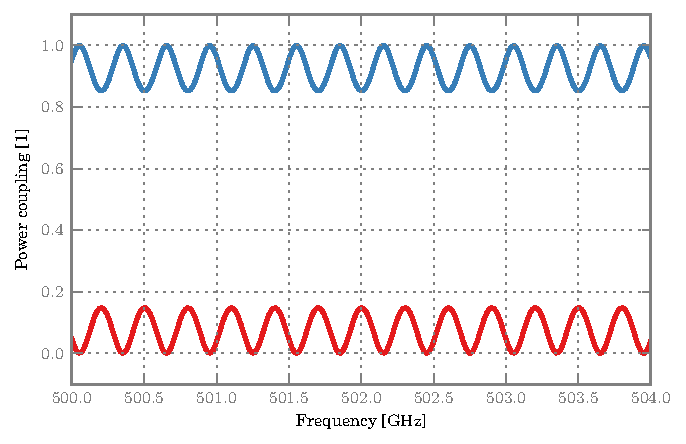
\includegraphics{simple_cavity_direct}
    \caption{Simple cavity, model result.}
    \caption*{
        The blue curve, on top, corresponds to the power coupling of port~6,
        that is the transmission through the cavity.
        The red curve, on the bottom, corresponds to the power coupling of port~1,
        that is the reflection on the cavity.
    }
    \label{fig:simple_cavity_direct}
\end{figure}
\begin{figure}[hbtp]
    \centering
    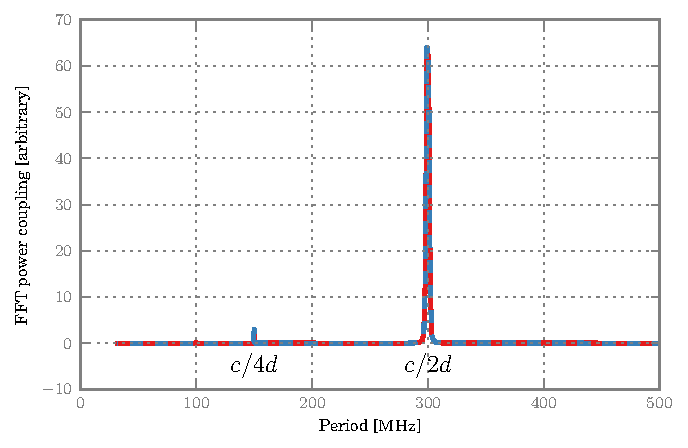
\includegraphics{simple_cavity_fft}
    \caption{Simple cavity, Fourier transform of the model result.}
    \caption*{
        The transmitted (blue) and reflected (red) wave show the same amount of modulation
        introduced by the cavity.
        The fundamental is at a period $F=c/2d$ with $c$ the speed of light in the cavity
        and $d$ the length of the cavity.
        An harmonic shows at $F=c/4d$,
        proving that the modulation is not perfectly sinusoidal.
        This spectrum was obtained by running the model for 4001 frequencies
        over a~\SI{64}{\giga\hertz} range,
        multiplying the result by a hanning window and taking a fast Fourier transform.
    }
    \label{fig:simple_cavity_fft}
\end{figure}

\Cref{fig:simple_cavity_direct} presents the result of the model for the following parameters:
\begin{itemize}
    \item refractive index $n_1=1.5$,
    \item refractive index $n_2=1.0$,
    \item distance between the interfaces $d=\SI{0.5}{\meter}$,
    \item frequency $f$ from \SIrange{500}{504}{\giga\hertz}.
\end{itemize}
The scattering matrices of the interfaces are derived from~\vref{eq:s_interface_normal} using $n_1$ and $n_2$.
The scattering matrix of the space between the interfaces is derived from~\vref{eq:scattering_distance} using $d$, $n_1$ and $f$.



%-----------------------------------------------------------------------------

\subsubsection{Periodicity}
According to \cref{eq:cavity_period}, we expect a periodicity of $F=c/2d$ where $c=c_0/n$ is the speed of light in the cavity and $d$ the length of the cavity.
With $c_0\approx \SI{2.998e8}{\meter\per\second}$, $n=1$ and $d=\SI{0.5}{\meter}$, we get $F \approx \SI{299.8}{\mega\hertz}$.

Our model agrees with our expectation, as shown by the fourrier transform in \cref{fig:simple_cavity_fft}.



%-----------------------------------------------------------------------------

\subsubsection{Energy conservation}
Examination of the results displayed in \cref{fig:simple_cavity_direct} reveals that energy is neither created nor destroyed.
The power is always positive, and the sum of the transmitted (blue) and reflected (red) power always equal 1 within numerical noise.
The power that is not transmitted through the cavity is reflected back to the source.



%=============================================================================

\subsection{Thin film beam splitter}

A thin dielectric film can be used as a beam splitter, as illustrated in \cref{fig:beam_splitter_principle}.
\begin{figure}[hbtp]
    \centering
    \input{beam_splitter_principle.pdf_tex}
    \caption{Beam splitter, principle.}
    \label{fig:beam_splitter_principle}
\end{figure}

This setup is one of the simplest way to inject local oscillator (LO) and sky signal together on a mixer.
What we have here is a heterodyne telescope.
The very transparent thin film couples most of the sky signal to the mixer, while coupling almost none of the local oscillator noise.
Unfortunately, the thin film is also transparent to the LO signal (narrow line at the LO frequency) required to pump the mixer, so the LO signal must be very strong.
This design wastes most of the LO power but has the advantage of being simple.
HIFI uses a similar approach for its bands 1, 2 and 3 (with wire grid polarizers instead of thin films though).

%-----------------------------------------------------------------------------

\subsubsection{Modeling the networks}

We can model the thin film using the principle described in \cref{sec:thin_film_at_oblique_incidence}.
Let us model a thin film of biaxially-oriented polyethylene terephthalate or ``boPET'', more commonly known under trade-mame ``Mylar''.
The table entry for ``PETP'' in the article of \citeauthor{lamb1996miscellaneous}~\cite{lamb1996miscellaneous} suggests that we choose 1.83 for the refractive index of the film at~\SI{500}{\giga\hertz}.
Using the notations of the article,
this 1.83 corresponds to the real part~$n$ of the refractive index~$\hat{n}=n-ik$.
The imaginary part~$k$ is given by the ``$\tan \delta$'' column of the table and
the equation (6) of that article, which links $\tan \delta$ to $k$: $\tan \delta = 2k/n$.
Therefore, $k = (n \tan \delta) / 2$.
With $n=1.83$ and $\tan \delta = 0.020$, we have $k=0.018$.
Our own conventions (deriving from~\cref{eq:e_z_t_real_minus}) require a sign flip: as explained in \vref{sec:polar_complex_notation}, a positive imaginary part creates absorption.
The complex refractive index of our thin film is $1.83+0.018i$.

% I know that the imaginary part of the refractive index corresponds to an absorption/gain.  The plus or minus sign probably depends on the convention chosen for k and omega.
% I have
% E = E_0 exp(ikz)
% k = \tau / \lambda
% \lambda = c / f
% c = c_0 / n
% k = \tau f n / c_0 = K n
% n = nr + i ni
% exp(iKnz) = exp(i K nr z - K ni z) = exp(iKnrz) exp(-Kniz)
% The greater ni, the stronger the attenuation.
% Therefore, I must keep ni positive.

To model the local oscillator and the mixer, I use networks that reflect \SI{10}{\percent} and transmit \SI{90}{\percent} of the incoming signal.
This is a very simplified model for a mixer or a local oscillator, but it does take into account their principle characteristic from a standing wave point of view: they reflect.

The two absorbers do not need any modeling: it is sufficient to leave the two corresponding ports of the thin film open.

%-----------------------------------------------------------------------------

\subsubsection{Simulation}
\begin{figure}[hbtp]
    \centering
    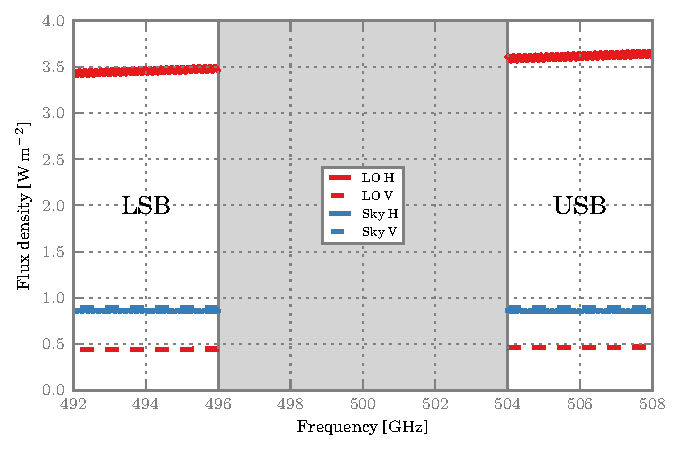
\includegraphics{thin_film_beam_splitter_detailed}
    \caption{Thin film beam splitter, detailed}
    \label{fig:thin_film_beam_splitter_detailed}
\end{figure}
In the lower and upper side bands, the mixer receives power from two sources: the astronomical signal from the sky and the noise of the local oscillator.
In the case of HIFI, the local oscillator noise is typically two orders of magnitude stronger than the astronomical signal.
We arbitrarily set the power density from the sky at \SI{1}{\watt\per\meter\squared} and that of the local oscillator to \SI{100}{\watt\per\meter\squared}.
Since these two sources are not phase locked, we solve the system for each of them independantly.
The result is given on \cref{fig:thin_film_beam_splitter_detailed}.

We notice that the power of both the local oscillator signal and the sky signal have the same order of magnitude when hitting the mixer.
This is due to the fact that the thin film is mostly transparent, hardly reflective.
Because the sky is seen in transmission, its power is still very close to its emitted value of \SI{1}{\watt\per\meter\squared}, we couple most of the sky.
And because the local oscillator is seen in reflection, we couple only a small fraction of it (\SI{0.5}{\percent} or \SI{3.5}{\percent} depending on the polarization).
This increases the signal-to-noise ratio to an acceptable level.

The figure also illustrates that this beam splitter transmits V more than it transmits H.
As a result, V shows more sky power and less LO power.
It is in the interest of the astronomer to reject the horizontal polarization.
This can be done with a wire-grid polarizer or by using rectangular horns.

When examined closely, the H curves show some fast oscillations.
The V curves are also affected, as the next figure will show.
These oscillations are due to the cavity formed by the mixer and the local oscillator.
That cavity consists of $d=\SI{1}{\meter}$ or vacuum, which results in a period of $c_0 / 2d \approx \SI{150}{MHz}$.

The red curves show a slope.
The higher the frequency, the more LO power the mixer sees.
This slope is actually a portion of a very slow standing wave pattern.
It corresponds to the cavity formed by the two interfaces of the thin film itself.
With a speed of light of $c_0 / 1.83$ and a thickness of \SI{10}{\micro\meter}, we expect a standing wave pattern with a period of about \SI{8}{\tera\hertz}.
Calculating the real period involves knowing the pathlength of the beam inside the film, which requires some trigonometry, but the order remains at several terahertz.

In a real system, we would not have access to all the details of \cref{fig:thin_film_beam_splitter_detailed}.
Indeed, for a given frequency, we receive the sum of the LO and sky power without being able to tell them apart.
Furthermore, mixers fold spectra, which adds the lower and upper side bands together.
Finally, the polarizations become undistinguishable.
In \cref{fig:thin_film_beam_splitter_folded}, we have summed the two sources and folded the spectra; however we kept the polarization intact.
These summations were done in power and not in field, because the LSB, USB, LO and sky power are not phase locked to each other: each signal is coherent with itself only, not with the others.

\begin{figure}[hbtp]
    \centering
    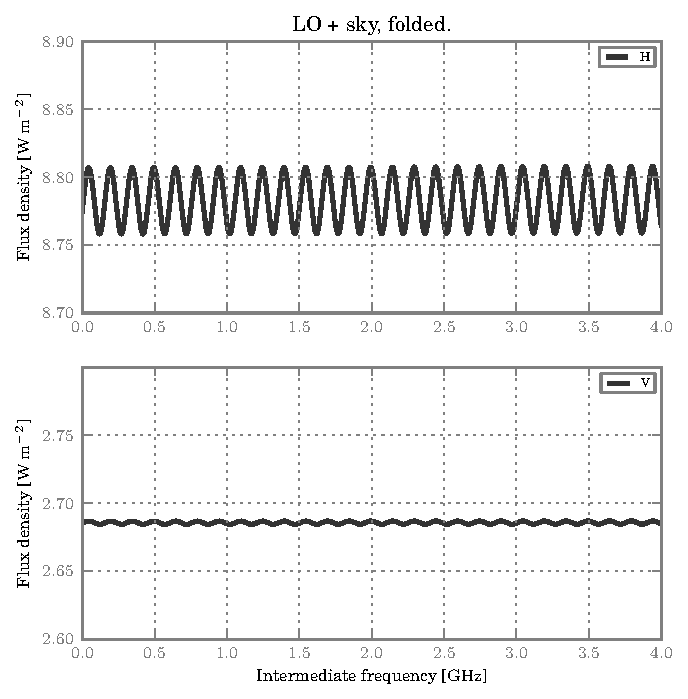
\includegraphics{thin_film_beam_splitter_folded}
    \caption{Thin film beam splitter, folded}
    \label{fig:thin_film_beam_splitter_folded}
\end{figure}

The slope due to the cavity inside the thin film seems to have disappeared.
This is expected: the lower sideband is flipped before being added to the upper sideband.
Therefore, when the slope goes up for one, it goes down for the other,
and they compensate quite well.
Some other values for the LO frequency or film thickness can allow the thin film cavity to leave a more obvious signature on the folded spectrum.

This figure reveals that the V polarization is also affected by standing wave, as we mentionned earlier.
It is much weaker in V than in H because the thin film is more transparent for V.
This means that the V-polarized light is more likely to exit the cavity either toward the sky or toward the open port on the right, both perfect aborbers.
This standing wave pattern has a period of \SI{150}{\mega\hertz}, which is expected of the LO--mixer cavity.

\subsubsection{Sideband ratio}
Standing waves change the coupling of the mixer to the signal.
This coupling is a priori different in the lower and upper sideband.
Therefore, each channel of a folded spectrum is a priori imbalanced, giving more weight to either sideband.

In the HIFI consortium, we agreed on the following definition~\eqref{eq:sideband_ratio} of the sideband ratio as a metric for the imbalance between the two sidebands.
A perfectly balanced system has a sideband ratio of 0.5.
If the sideband ratio is greater than 0.5, then the channel is USB-dominated.
If it is lower than 0.5, the channel is LSB-dominated.
\begin{equation}
    \text{sideband ratio} =
    \frac{
        \text{USB power coupling}
    }{
        \text{LSB power coupling} + \text{USB power coupling}
    }
    \label{eq:sideband_ratio}
\end{equation}

\begin{figure}[hbtp]
    \centering
    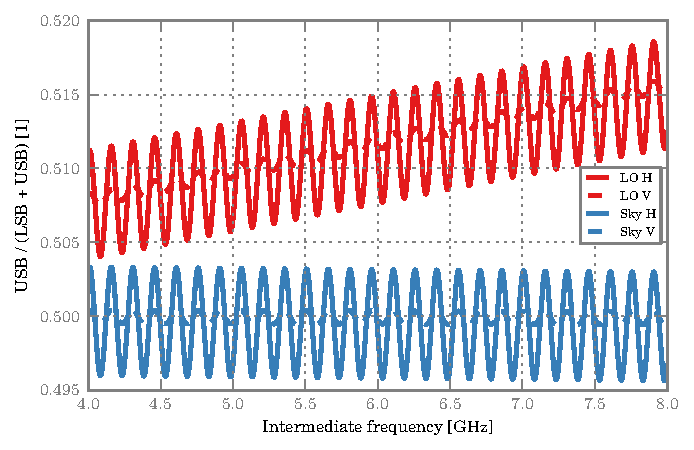
\includegraphics{thin_film_beam_splitter_sbr}
    \caption{Thin film beam splitter, sideband ratio}
    \label{fig:thin_film_beam_splitter_sbr}
\end{figure}
\Cref{fig:thin_film_beam_splitter_sbr} shows the sideband ratio for the LO and the sky for both polarizations.
The slope comes from very slow modulation due to the cavity inside the thin film.
Note that it is clearly visible here, even on the sky, while it was hardly noticeable on the folded spectrum of \cref{fig:thin_film_beam_splitter_folded}.
A flat continuum does not guarantee a flat sideband ratio.

With this system, the standard deviation of the sideband ratio for is \SI{2.6}{\percent} for H and \SI{0.3}{\percent} for V.
This is the error that we can expect when measuring a thin emission line on a perfectly flat continuum after an infinitely long integration time: the line can fall anywhere between a peak and a crest of this standing wave pattern.

\subsubsection{The many LO--mixer cavities}

\Cref{fig:thin_film_beam_splitter_folded_fft} shows
the fast Fourier Transform of \cref{fig:thin_film_beam_splitter_folded} (using a Hanning window).
It peaks at the expected~\SI{150}{\mega\hertz} and shows a very weak harmonic at~\SI{75}{\mega\hertz}.
The harmonics are very weak because the cavity is of very low quality: the film is very transparent and the light leaves the cavity quickly.

\begin{figure}[hbtp]
    \centering
    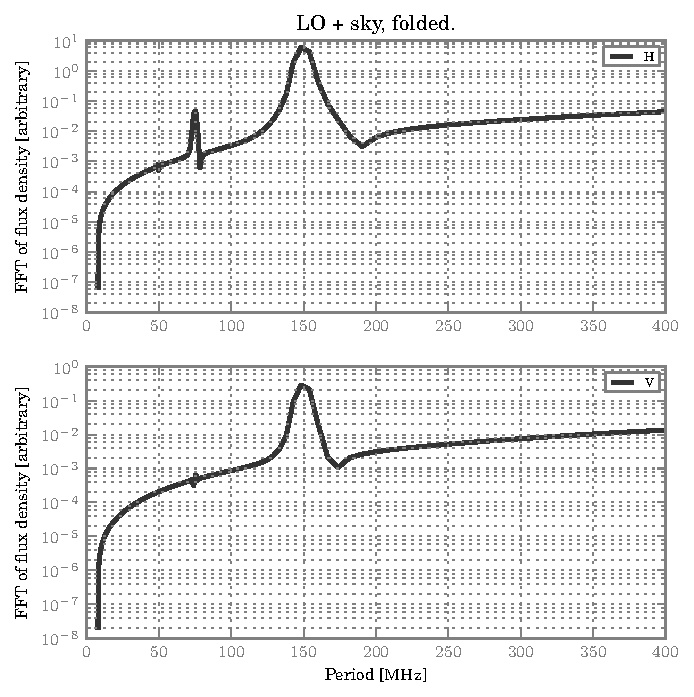
\includegraphics{thin_film_beam_splitter_folded_fft}
    \caption{Thin film beam splitter, folded, fft}
    \label{fig:thin_film_beam_splitter_folded_fft}
\end{figure}

The astute reader may be wondering why we are observing only two cavities (LO--mixer and inside thin film) instead of an infinity.
Indeed, there is no such thing as \textit{the} LO--mixer cavity, there are an infinity of them.
The shortest one is the one corresponding to a single reflection on the near side of the thin film.
Then, another possible path involves entering the thin film, being reflected by the far side, traversing the film again, and being transmitted toward the detector.
A third path involves two round-trips inside the film, and a fourth path involves three round-trips, etc.
Why don't these many cavities show up as as many peaks on the FFT?
The answer is simple: our FFT does not have enough resolution.

Our bandpass $B$ of \SI{4}{\giga\hertz} does not allow to resolve a variation of \SI{10}{\micro\meter} in a cavity.
$B = c / 2d$ with $d=\SI{10}{\micro\meter}$ and $c=c_0$ yields $B \approx \SI{15}{\tera\hertz}$, which is way beyond our \SI{4}{\giga\hertz}.
If we reverse the calculation, $d=c/2B$ for $B=\SI{4}{\giga\hertz}$ gives $d \approx \SI{37}{mm}$: our FFT can distinguish cavities that differ by more than \SI{4}{\centi\meter}.
This limitation affects only the FFT as a tool used for visualizing our data; our model has no such limitation.

\begin{figure}[hbtp]
    \centering
    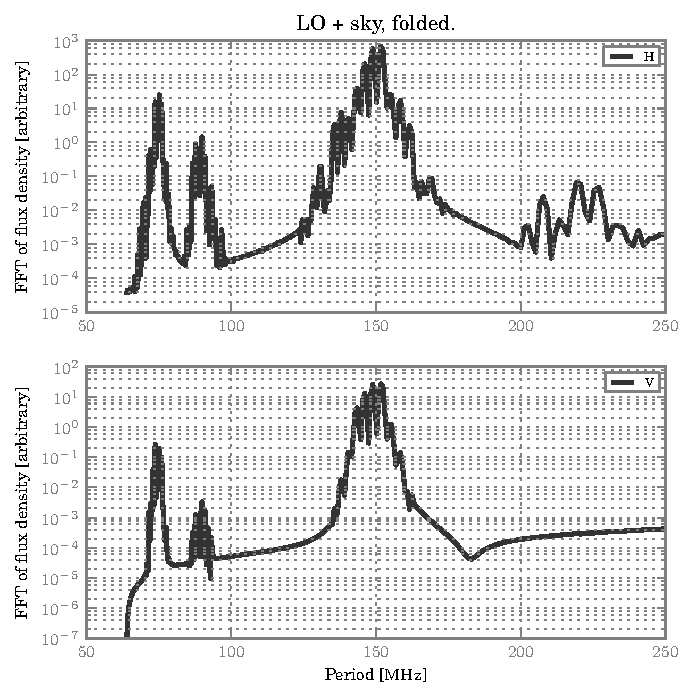
\includegraphics{thin_film_beam_splitter_folded_fft_hr}
    \caption{Thin film beam splitter, folded, fft, high resolution}
    \label{fig:thin_film_beam_splitter_folded_fft_hr}
\end{figure}
\Cref{fig:thin_film_beam_splitter_folded_fft_hr} shows the FFT of the same system for a bandwidth of~\SI{32}{\giga\hertz}, a film thickness of~\SI{1}{\centi\meter}, and no imaginary part in the refractive index of the mylar (otherwise the absorption would hide the result).
Once the system is modified to meet the expectations of the FFT, then the FFT does show the expected many peaks around~\SI{150}{\mega\hertz}, which prove that our model takes into account the infinity of LO--mixer cavities.


\cleardoublepage
\chapter{Parametric study of HIFI's standing waves}
\section{Model used to explore the parameters}
In this part, I use HIFI as an example.
My goal is to show where each standing wave in HIFI is born.

\section{Folding and calibration}

We are going to assume that the intrinsic sideband ratio of the mixer is 0.5, that is that the mixer is perfectly balanced.  This is of course not the case, but our goal here is to explore the effect of the standing waves on the coupling, not the imperfections of the mixer.

\section{Exploration}

At first, the whole system will be as perfect as I can make it.  I do not have a model for a perfect grid, but I can make the grid so thin and dense that it will drown the effect of the grid within the thickness of the line in the plots.

Then, little by little I will make the elements more realistic, and describe the results.

Each time, I present a plot of
\begin{itemize}
    \item the coupling of the mixers to the LO before mixing,
    \item the coupling of the mixers to the sky before mixing,
    \item the coupling of the mixers to the LO after mixing,
    \item the coupling of the mixers to the sky after mixing,
    \item the sideband ratio.
\end{itemize}
Whenever possible, I must refer to HIFI data exhibiting this kind of feature.

\subsection{Entry grid}
We have to expect a slightly different H/V ratio on each side of the grid.
Plus, the amount of power may be different too.

By zooming on the Y axis of the plots, I show that the higher the frequency, the more the grid leaks.  This is not surprising.

\subsection{Perfect instrument}
Even in the perfect case, the diplexer is optimally tuned to the center of the IF, and there is a twenty-percent degradation of the coupling at the borders of the IF.

Show that there is a slight offset of the perfect diplexer tuning due to the entry grid not being perfect.

This means that we are correct in taking calibration measures in order to tune the diplexer instead of relying on the value given by the formula.

\subsection{Reflective co-pol mixer}
Turning on the co-pol reflectivity of the mixer simulates the imperfection of the horn.

\subsection{Reflective cross-pol mixer}
This simulates a desired behavior of the horn: the crosspol must not couple to the mixer.
Well, it would be nice if the crosspol would just disappear, but it is not how rectangular horns work, they reflect what they don't want.

\subsection{Reflective co- and cross-pol, standing waves}
As soon as one reflection is turned on, we observe a standing wave pattern.
This is a priori paradoxical.
Indeed, for standing waves to appear, a cavity must exist, that means we need two reflective surfaces and we have only one.

We show that the mixer is actually looking at itself through the leaky grid of the diplexer unit.

\subsection{Blaming the grids}
We make the grid much thinner and denser, and the standing wave patters from the previous subsection disappears.

We make the grid coarser and it gets worse.

There is a limit on how coarse you can make the grid, as the grid model my Houde makes assumptions on the radius of the wires, their spacing, and the wavelength.

With insanely bad grids, we show that the standing wave pattern is actually far from sinusoidal, as the cavity has a very high Q.

\subsection{Imperfect rooftop mirrors}
This is how we can achieve the first exchange of polarization power.
Indeed, if we make only the co-pol of the mixer reflective, with an imperfect roof-top mirror we observe standing wave patters on the two polarizations.

We can also observe a beat of the standing wave patterns.  This is due to the two arms of the diplexer units being of different length.  A fourrier transform can reveal two picks.
In fact, every cavity involving the diplexer will show these picks.

\subsection{Turn on the LO reflection}
This creates a very strong modulation on top of all the others.
This also allows the two mixers to see each other.
Indeed, because the entry grid leaks, some standing wave patters in one polarization will affect the other after reflection on the local oscillator.

\subsection{Effect of the attenuator in front of the local oscillator}
Reduces the cross talk and the LO standing waves.

\subsection{Simulated diplexer scans}
These reproduce distorsions observed on real diplexer scans.

\subsection{Influence of the diplexer tuning on the cross talk}
Show that mistuning one diplexer has an effect on the coupling of the mixer in the other branch.


\cleardoublepage
\chapter{HIFI Standing wave calibration}
\cleardoublepage
%\begin{refsection}
\chapter{Interference model of HIFI Band~1}
\label{sec:chapter4}


%#############################################################################
\section{Introduction}
The previous chapters describe a physically-based model that we created to predict the effect of interferences in coherent detectors.
This chapter compares our model to observational data from the HIFI instrument~\parencite{AA_518_L6}.
Our goal is to validate our model and to derive parameters several system parameters for the HIFI instrument that are only approximately known from its design and commissioning.

We choose to model HIFI Band~1.
Bands~1, 2 and 5 of HIFI have fewer optical elements than Bands~3, 4, 6 and 7, making them easier to model by reducing the number of free parameters.
Indeed, Bands~3, 4, 6 and 7 use rooftop mirrors to form Martin--Puplett interferometers in order to maximize the coupling of the mixer to the sky and the local oscillator at the same time.
In Bands~1, 2 and 5, the LO power is high enough and there is no need to maximize its coupling to the mixer, allowing for a simpler design with less side-effects.
The coupling of the LO to the mixer is very weak in Band~1, which means that the LO--mixer cavities produce almost no interference;
this reduces again the number of parameters.
\Textcite{risacher2011standingwaves} confirms that the LO--mixer ripples are not detected in Band~1.

In a typical observation, HIFI takes four measurements: one on the source of astronomical interest, one on a part of the sky devoid of emission, and one on the hot and cold internal calibration loads.
The integrations on the loads are used to calibrate the bandpass of the instrument.
Ideally, the loads are black bodies, which means that they are perfect absorbers.
In practice, the loads are not perfect black bodies but reflect a fraction of the incident electromagnetic waves.
Likewise, the mixer reflects a fraction of the incident wave.
These reflections create interferences that impact the bandpass calibration of the instrument and results in ripples on the spectra.




\begin{figure}
    \centering
    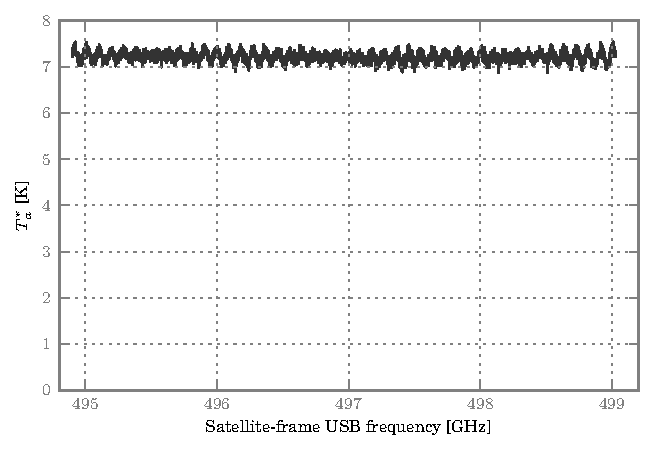
\includegraphics{mars_25_original}
    \caption{Observation of Mars by HIFI in Band~1 with the WBS-H showing a continuum modulated by ripples.
    Source: HSA, obsid 0x2fb00eb.}
    \label{fig:mars_25_original}
\end{figure}

\Cref{fig:mars_25_original} shows a HIFI observation of the planet Mars recorded in Band~1 by the WBS-H backend, the wide-band spectrometer, horizontally polarized.
This spectrum has no line, and its continuum is modulated by ripples.
Atmospheric models of Mars predict a flat continuum, therefore we can attribute these ripples to an instrumental artifact that the calibration does not correct: interferences.
We choose this spectrum to validate our model because the ripples are relatively strong compared to the thermal noise present in the observation.
In this chapter, we use these ripples to derive the position of the loads, their reflection coefficient, and that of the mixer.

We begin the chapter with a brief description of the optics of HIFI Band~1.
Then we proceed to model the ripples in two steps.
First, we create a semi-analytic model, in which we model the ripples using ad-hoc perfect sinusoids.
This model gives us the periods of the ripples, which we can convert into approximate distances.
Second, we create a physically-based numerical model using the method detailed in~\cref{sec:chapter2}.


%#############################################################################
\FloatBarrier



\section{HIFI Band 1}
\Cref{fig:band1_layout} presents the optical layout of Band 1 of HIFI.
The signal from the local oscillator and the signal from the source are combined by a wire grid polarizer.
Two mixers detect the resulting beams.

Waves polarized in the plane of the page are called ``vertically polarized'' while waves polarized normally to the page are called ``horizontally polarized''.
The ``H~mixer'' detects horizontal waves, and the ``V~mixer'' detects vertical waves.

\begin{figure}
    \centering
    \footnotesize
    \input{band1_layout.pdf_tex}
    \caption{Layout of the optics of Band~1}
    \label{fig:band1_layout}
\end{figure}

Two wire grid polarizers ensure that the waves propagating toward the mixers are properly polarized for an optimal coupling to the mixer: they are noted ``H~grid'' and ``V~grid'' on the figure.
The wires of the H~grid are normal to the plane of the page and those of the V~grid lie in the plane of the page.
Grids are four-port devices (see~\cref{sec:wire_grid_polarizer}), two ports of each grids are dumped onto an absorber, getting rid of any unwanted polarization.

Three mirrors focus the beam from the grids into the horns of the mixers.

The signal from the sky is not polarized.
The thermal noise from the local oscillator and the calibration loads is not polarized either.
However, the useful signal of the local oscillator, that which pumps the mixers, is vertically polarized.

In Band~1, the local oscillator produces a beam whose power is much too high to properly pump the two mixers; most of the LO power needs to be dumped.
This is achieved by slightly rotating grid-0: its wires make an angle of~\SI{5.7}{\degree} with the plane of the page.
With that configuration, grid~0 sends most of the LO power down the H path, where it mostly goes through the H~grid into the dumps, and only a small fraction reaches the H~mixer.
The small fraction of LO power sent down the V~path by grid~0 is mostly reflected by the V~grid toward the V~mixer.
In the end, each mixer sees about~\SI{1}{\percent} of the LO power, the right amount of power to pump them optimally.

This very low coupling between the mixers and the local oscillator has an advantage: the LO--mixer cavities are very lossy and the interferences that they create are likely to be negligible.
In addition, the local oscillator itself is equipped with a~\SI{10}{\decibel} attenuator, which reduces interferences even more.
As a result, we expect that most of the ripples are caused by interferences in the cavities formed by the mixers and the calibration loads.
The coupling between the mixers and the local oscillator is greater in Bands~2 and 5; modeling them requires more parameters to account for this.





%#############################################################################
\FloatBarrier



\section{Analysis of the ripples}



%=============================================================================

\subsection{Smoothing}
In order to make the ripples more apparent, we smooth the original spectrum.
We do so by zeroing all power at periods shorter than a given threshold (\SI{40}{\mega\hertz} in our case).

\Cref{fig:mars_filtered} shows the result of that smoothing.
The original data is shown in black, the smoothed data in green and the residual in gray.

\begin{figure}
    \centering
    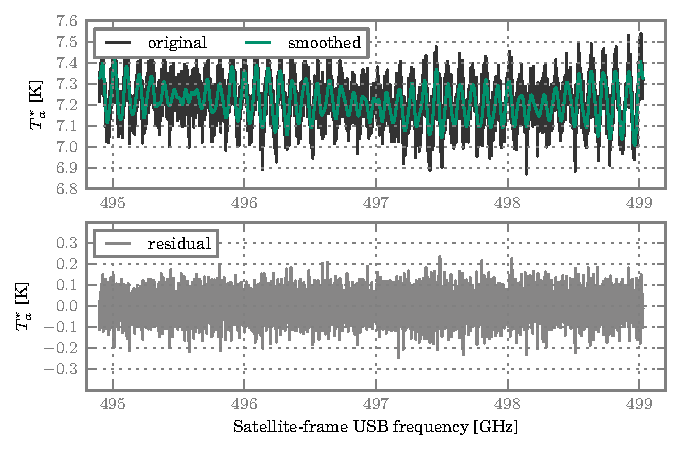
\includegraphics{mars_25_smoothed}
    \bigskip
    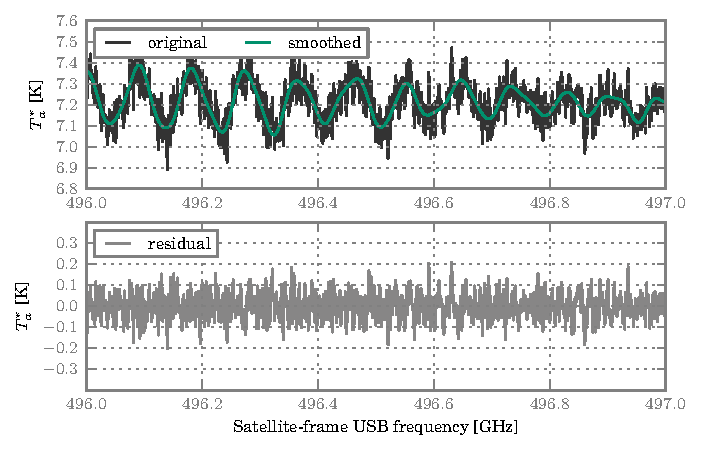
\includegraphics{mars_25_smoothed_zoom}
    \caption{
        Smoothing the spectrum of Mars separates the ripples from other sources of noise.
        Top: full spectrum, \SI{4}{\giga\hertz}-wide.
        Bottom: zoom on a \SI{1}{\giga\hertz}-wide region.
    }
    \label{fig:mars_filtered}
\end{figure}

The smoothed curve appears as a sinusoid wrapped in a sinusoidal envelope.
This ``beat'' pattern is typically produced when two sines of different but close periods are added together.
We are therefore expecting the contribution of two ripples, each coming from one cavity.
The period of the ripples, about~\SI{100}{\mega\hertz}, is compatible with the distance of about~\SI{1.5}{\meter} that separate the calibration loads from the mixer.
%\todo[inline]{Ref for the mixer--load distance, it's not easy to find, we mostly know it from previous standing waves analysis}
Indeed, the length~$d$ of a cavity and the period~$F$ of the ripple that it produces are linked by
the relation
\begin{equation}
    d = \frac{c}{2F}
    \label{eq:relation_length_period}
\end{equation}
in which $c$ is the speed of light in the medium, which we assume to be vacuum.
This equation is a rewrite of~\vref{eq:relation_length_period_nice}, in which the speed of light is made explicit.

An ideal spectrum for our purpose would combine a strong continuum, no spectral line, strong ripples and a low noise; but such spectra have little astronomical value and are therefore extremely rare, if at all present, in the HIFI database.
This spectrum shows very strong ripples which are helpful to constrain some parameters of our model.
Unfortunately, the thermal noise on top of these ripples is also very strong.
Indeed, the integration time of this observation is quite short: this observation was not designed to measure the continuum of Mars but to calibrate the pointing of the satellite.

%\begin{table}
%    \centering
%    \begin{tabular}{lc}
%        \toprule
%        spectrum & standard deviation [\si{\kelvin}]\\
%        \midrule
%        original & 0.101\\
%        smoothed & 0.080\\
%        residual & 0.061\\
%        \bottomrule
%    \end{tabular}
%    \caption{There is almost as much energy in the noise (residual) as in the ripples (smoothed).}
%    \label{tab:mars_filtered_stddev}
%\end{table}



%=============================================================================

\subsection{Fourier Transform}
Ripples are quasi-periodic features.
As such, they appear as peaks on a Fourier Transform.
\Cref{fig:mars_25_dft} shows the Discrete Fourier Transform of the spectrum of Mars.

\begin{figure}
    \centering
    \hfill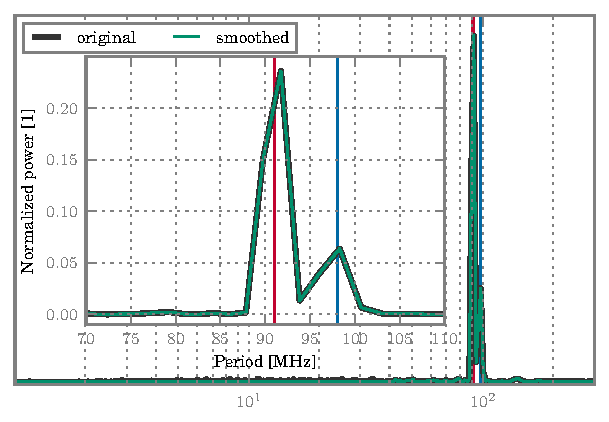
\includegraphics{mars_25_dft_lin}\\
    \hfill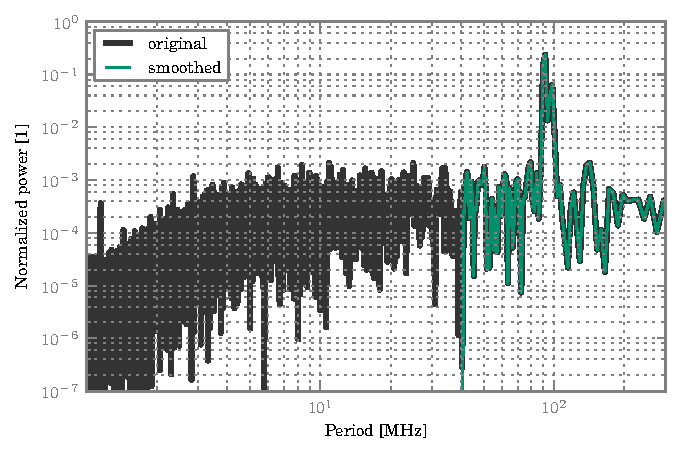
\includegraphics{mars_25_dft_log}
    \caption{
        Direct Fourier Transform of the original Mars spectrum (black) and its smoothed version (green).
        The inner plot zooms onto the two peaks.
        The vertical lines mark the approximate periods of the hot (red) and cold (blue) ripples.
        Top: linear vertical scale.
        Bottom: logarithmic vertical scale.
    }
    \label{fig:mars_25_dft}
\end{figure}

The horizontal axis of \cref{fig:mars_25_dft} represents the periods: short-period features are on the left, long-period features are on the right.
The continuum is not represented as it has an infinite period.
The vertical axis is either linear (top plot) or logarithmic (bottom plot).
In both cases, the vertical axis represents the power present at a given period.
Since our goal is to locate peaks, and not measure their power, the vertical axis has been normalized.

With its linear axis, the top plot shows that most of the power is concentrated into two peaks that are located at approximately~\SI{91}{\mega\hertz} and~\SI{98}{\mega\hertz}, marked by the red and blue vertical lines.
The resolution of the Fourier Transform is low at these periods, one would need spectra with a much broader frequency coverage to resolve these peaks.
The bottom plot is interesting because it shows no evidence of harmonics.
The fundamentals are located at~\SI{91}{\mega\hertz} and \SI{98}{\mega\hertz}, we could expect harmonics peaking at half these periods, and even weak harmonics would stand out on a logarithmic scale.
The lack of visible harmonics suggests that the cavities that create the ripple are very lossy (see~\cref{sec:fabry_gain}).

These plots in the Fourier domain bring evidence that we can model the ripples as two perfect sinusoids.



%=============================================================================

\subsection{Perfect-sines model}
\label{sec:perfect_sines_model}
Examining the Direct Fourier Transform of the spectrum shows evidence of two sinusoidal ripples but offers only a crude approximation of their period.

To determine the periods of the ripples more accurately, we model the smoothed spectrum with three components: a polynomial of degree 1 for the baseline and two sinusoidal functions.

The baseline is modeled with~$y=a(f-f_0)+b$ where
$f$ the frequency of the channel and
$f_0=\SI{496974750000}{\hertz}$ is the frequency in the middle of the spectrum.
Each ripple is modeled with~$y = C \cos(\phi) + S \sin(\phi)$ where
$\phi = 2 \pi f / F$ and $F$ is the period of the sine.

The model parameters are given in \cref{tab:two_sines_fit}.
This model gives us a much better estimate of the periods of the ripples than the one provided by the DFT.
\Cref{fig:mars_sine_fit} illustrates the differences between the smoothed spectrum of Mars and its model using perfect sines.


\begin{table}[b]
% Cont result ['7.211908771679127', '-1.262493598126238e-11']
% Cont errors ['5.614822816527074e-05', '4.7109413498749796e-14']
    \centering
    \begin{tabularx}{\textwidth}{X c c}
        \toprule
            &
            slope $a$ [\si{\kelvin\per\hertz}]
            &
            average $b$ [\si{\kelvin}]
            \\
        \midrule
            baseline
            &
            $\num{-1.262e-11} \pm \num{4.7e-14}$
            &
            $\num{7.21191} \pm \num{5.6e-05}$
            \\
        \bottomrule
    \end{tabularx}\\
    \bigskip
% Hot  result ['-0.024374668042950198', '-0.084177761411197496', '90964727.019958138']
% Hot  error  ['0.032581863729936822', '0.0094248123566952492', '1025.6247261452409']
% Cold result ['-0.03334118353679541', '-0.039445727877105055', '97604192.684090942']
% Cold error  ['0.026008970168651415', '0.021974915562550285', '2011.3533923905459']
    \begin{tabularx}{\textwidth}{X c c c}
        \toprule
        ripple
        &
            $\cos$ amplitude $C$ [\si{\kelvin}]
        &
            $\sin$ amplitude $S$ [\si{\kelvin}]
        &
            period $F$ [\si{\hertz}]
        \\
        \midrule
        hot &
        $\num{-0.01965} \pm \num{0.00055}$ &
        $\num{ 0.08539} \pm \num{0.00013}$ &
        $\num{90964800} \pm \num{1000}$ \\
        cold &
        $\num{-0.03658} \pm \num{0.00032}$ &
        $\num{ 0.03645} \pm \num{0.00032}$ &
        $\num{97604400} \pm \num{2100}$\\
        \bottomrule
    \end{tabularx}
    \caption{
        Parameters modeling the baseline and the ripples of the smoothed spectrum of Mars with a polynomial and two sinusoids.
    }
    \label{tab:two_sines_fit}
\end{table}

\begin{figure}
    \centering
    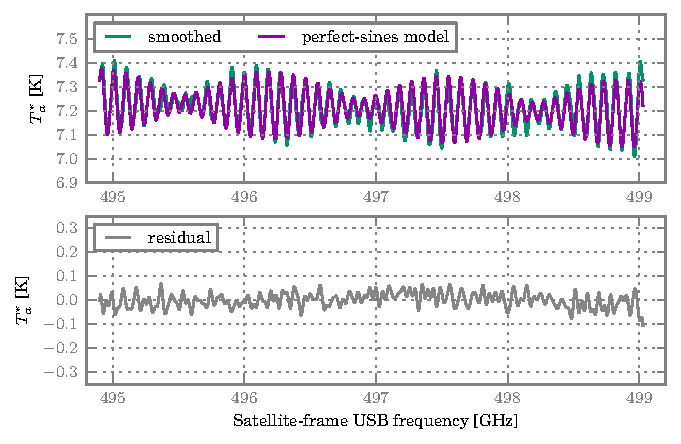
\includegraphics{mars_25_sine_fit}
    \caption{Model of the ripple using two sinusoids.}
    \label{fig:mars_sine_fit}
\end{figure}

Using~\cref{eq:relation_length_period} with $c=c_0$ (the speed of light in vacuum), we get our first estimate of the length of the cavities which we give in~\cref{tab:first_estimate_cavity_length}.
The mixer and the hot load are separated by~\SI{1.64}{\meter}, the mixer and the cold load by~\SI{1.53}{\meter}.
These are optical path lengths, not actual distances.
Assuming~$c=c_0$ is justified by the fact that the focal plane unit of HIFI is in vacuum.
However, this assumption suggests that there is only vacuum between the loads and the mixers, which we know is not the case since there are two grids and three mirrors in that optical path.
Furthermore, the surface of a load is a mathematical one: a load does not present a perfectly plane surface normal to the beam; we assume that the load behave as if it had an effective plane surface at a given effective distance.
For these two reasons, we expect that the optical path lengths that we just calculated differ somewhat from the actual distances between the mixers and the loads.

\begin{table}
    \centering
    \begin{tabular}{lcc}
        \toprule
        ripple &
        period [\si{\hertz}] &
        pathlength [\si{\meter}] \\
        \midrule
        hot  & $\num{90964800} \pm \num{1000}$ & $\num{1.64785} \pm \num{0.00004}$ \\
        cold & $\num{97604400} \pm \num{2100}$ & $\num{1.53575} \pm \num{0.00006}$ \\
        \bottomrule
    \end{tabular}
    \caption{First estimation of the distance between the mixer and the loads, from the
    period of the ripples.}
    \label{tab:first_estimate_cavity_length}
\end{table}





%#############################################################################
\FloatBarrier



\section{Interference modeling of HIFI Band 1}
We apply the method of~\cref{sec:chapter2} to model the optics of HIFI.
We rely on this model to predict the interferences in the mixer--load cavities.

The interference model alone can only predict the gains of the system for a given input.
In order to reproduce the spectrum of Mars, we need to apply these gains to an input power.


First, we describe how we must calibrate the output of our model to reproduce the spectrum of Mars.
Then, we present the configuration of networks that we use to model the optics of Band~1 and predict its gains.
Finally, we determine the powers, and therefore electric field amplitudes, that enter our system.



%=============================================================================

\subsection{Calibration equation}

The spectrum of Mars shown in~\cref{fig:mars_25_original} is the result of the standard HIFI calibration pipeline \parencite{hifiobserversmanual}.
This pipeline applies the reference subtraction and the bandpass calibration described in \textcite{ossenkopf2002intensity}.
It is summarized by the following equation:
\begin{equation}
    J_\text{src}(f)% - J_\text{ref}(f)
    = 
    \frac{
        c_\text{src}(f) - c_\text{ref}(f)
    }{
        c_\text{hot}(f) - c_\text{cold}(f)
    }
    (\eta_\text{hot} + \eta_\text{cold} - 1)
    (
        J_\text{hot}(f_\text{LO}) - J_\text{cold}(f_\text{LO})
    )
    \text{.}
    \label{eq:mars_calibration}
\end{equation}
$J_\text{src}(f)$ is the spectrum plotted on~\cref{fig:mars_25_original}, it would correspond to the power detected from Mars expressed as a Rayleigh--Jeans temperature if the calibration had properly removed the ripples.
The four values $c_\text{src}$, $c_\text{ref}$, $c_\text{hot}$ and $c_\text{cold}$ correspond to the output of the spectrometer expressed in its native arbitrary unit (``CCD counts'' for the WBS) for the four pointings done during the observation:
on Mars (``src''), on the blank sky (``ref'') and on the hot and cold calibration loads.
The two terms $\eta_\text{hot}$ and $\eta_\text{cold}$ are the power coupling efficiencies of the beam to the calibration loads.
Finally, $J_\text{hot}$ and $J_\text{cold}$ refer to the power emitted by the calibration loads, expressed as Rayleigh--Jeans temperatures.

For this observation,
$f_\text{LO} = \SI{490.97475}{\giga\hertz}$,
$\eta_\text{hot} = 0.959$,
$\eta_\text{cold} = 0.991$,
$T_\text{hot} = \SI{100.275}{\kelvin}$ and
$T_\text{cold} = \SI{13.134}{\kelvin}$.

The last two parameters, $T_\text{hot}$ and $T_\text{cold}$ are the physical temperatures of the calibration loads measured by thermometers during the observation.
Assuming that the loads are black bodies, their spectral radiance $B$ follow Planck's law.
\begin{equation}
    B
    =
    \frac{2 h f^3}{c^2} \frac{1}{e^{\frac{h f}{k_B T} - 1}}
    \label{eq:planck_law}
\end{equation}
Here, $T$ is the temperature of the load, $f$ is the frequency, $h$ is Planck's constant, $c$ is the speed of light in the propagation medium (vacuum for us) and $k_B$ is the Boltzmann constant.
We want to express their spectral radiance as Rayleigh--Jeans temperatures $J_\text{hot}$ and $J_\text{cold}$.
We do this by solving Rayleigh--Jeans' law for $J$.
\begin{equation}
    B
    =
    \frac{2 f_\text{LO}^2 k_B}{c^2}J
    \label{eq:rayleigh_jeans_law}
\end{equation}
The results are $J_\text{hot} = \SI{88.95}{\kelvin}$ and $J_\text{cold} = \SI{4.70}{\kelvin}$.
We must remember that HIFI is a double-sideband instrument: each channel of the spectrum contains a contribution from both sidebands.
When looking at a continuum source at a temperature $J$, HIFI receives $J$ in each sideband for a total of $2J$.
To compensate, the scaling factor $J_\text{hot} - J_\text{cold}$ must be multiplied by 2.
This is equivalent to having $J_\text{hot} = \SI{177.90}{\kelvin}$ and $J_\text{cold}=\SI{9.40}{\kelvin}$.


Rayleigh--Jeans' law is an approximation of Planck's law for low frequencies and/or high temperatures.
The difference between $T_\text{hot}$ and $J_\text{hot}$ and between $T_\text{cold}$ and $J_\text{cold}$ illustrates that this approximation is poor in the range of powers and frequencies at which HIFI operates.
Nevertheless, it is customary for radioastronomers to express powers as Rayleigh--Jeans temperatures.

Since our goal is to reproduce a real observation of Mars with our model of the optics of HIFI Band~1, we use the same equation and the same parameters to calibrate our model.
Our model must provide $c_\text{src}$, $c_\text{ref}$, $c_\text{hot}$ and $c_\text{cold}$.
This is the subject of the next sections.



%=============================================================================

\subsection{IF chain}
The Intermediate Frequency (IF) chain processes the signal output by the mixer.
It consists in amplifiers, filters, and eventually a detector.
In our case, the detector is a pixel of the CCD of the WBS.
The output $c$ of the detector is an affine function of the power of its input $P_\text{detector input}$:
\begin{equation}
    c = G_\text{detector} \; P_\text{detector input} + z
\end{equation}
in which $G$ converts the unit from power to CCD count, and $z$ is an arbitrary constant.
The subtractions and the division in the calibration equation remove $G$ and $z$ from our concern.
\begin{equation}
    \frac{
        c_\text{src} - c_\text{ref}
    }{
        c_\text{hot} - c_\text{cold}
    }
    =
    \frac{
        P_\text{detector input, src} - P_\text{detector input, ref}
    }{
        P_\text{detector input, hot} - P_\text{detector input, cold}
    }
\end{equation}

Each power $P$ in the previous equation is proportional to the square of the amplitude of the electric field.
That coefficient of proportionality also disappears during the division.
\begin{equation}
    \frac{
        c_\text{src} - c_\text{ref}
    }{
        c_\text{hot} - c_\text{cold}
    }
    =
    \frac{
        \abs{\cp{e}_\text{detector input, src}}^2
        -
        \abs{\cp{e}_\text{detector input, ref}}^2
    }{
        \abs{\cp{e}_\text{detector input, hot}}^2
        -
        \abs{\cp{e}_\text{detector input, cold}}^2
    }
\end{equation}

Finally, the electric field at the input of the detector is proportional to the electric field at the output of the mixer:
$\cp{e}_\text{detector input} = \cp{g}_\text{IF chain} \cp{e}_\text{mixer output}$.
The division removes once again the common factor~$\abs{\cp{g}_\text{IF chain}}^2$.
\begin{equation}
    \frac{
        c_\text{src} - c_\text{ref}
    }{
        c_\text{hot} - c_\text{cold}
    }
    =
    \frac{
        \abs{\cp{e}_\text{mixer output, src}}^2
        -
        \abs{\cp{e}_\text{mixer output, ref}}^2
    }{
        \abs{\cp{e}_\text{mixer output, hot}}^2
        -
        \abs{\cp{e}_\text{mixer output, cold}}^2
    }
\end{equation}
In other words, we can completely ignore the IF chain.



%=============================================================================

\subsection{Mixing}
Although mixers are non-linear devices, their useful output phasor is proportional to their input phasor in the case of small signals (see~\vref{sec:mixer_model}).
\begin{equation}
    \begin{aligned}
    \cp{e}_\text{mixer output}
    &=
    \cp{g}_\text{mixer, LSB} \;
    \cp{e}_\text{mixer input, LSB} \\
    &+
    \cp{g}_\text{mixer, USB} \;
    \cp{e}_\text{mixer input, USB}
    \end{aligned}
\end{equation}
The frequency of the input phasors are $f_\text{LSB}$ and $f_\text{USB}$.
The frequency of the output phasor is $f_\text{IF}$.
The gain $\cp{g}_\text{mixer}$ is intrinsic to the mixer, it may depend on the frequency and be different for the LSB and USB frequency.

As this equation shows, mixers are coherent devices: they operate in field, not in power.
Although correct at any instant $t$, this equation cannot be applied to our situation.
Indeed, HIFI spectra are integrated over several seconds, which is orders of magnitude above the coherence time of the LSB and USB signals.
The LSB and USB signals are both coherent on their own, but they are not correlated with each other for that long: they are not phase-locked to each other.
The proper way of combining the contributions of the LSB and USB signals is in power:
\begin{equation}
    \abs{\cp{e}_\text{mixer output}}^2
    =
    \abs{\cp{e}_\text{mixer output, LSB}}^2
    +
    \abs{\cp{e}_\text{mixer output, USB}}^2
\end{equation}
with
\begin{align}
    \cp{e}_\text{mixer output, LSB}
    &=
    \cp{g}_\text{mixer, LSB}
    \;
    \cp{e}_\text{mixer input, LSB}
    \\
    \cp{e}_\text{mixer output, USB}
    &=
    \cp{g}_\text{mixer, USB}
    \;
    \cp{e}_\text{mixer input, USB}
    \text{.}
\end{align}

The standard HIFI pipeline assumes that the gain is the same for both sidebands:
$\cp{g}_\text{mixer, LSB} = \cp{g}_\text{mixer, USB} = \cp{g}_\text{mixer}$.
We make the same assumption in our model.
The resulting term $\abs{\cp{g}_\text{mixer}}^2$ disappears during the bandpass calibration.
With the subscript ``mi'' standing for ``mixer input'', we get the following equality.
\begin{gather}
    \frac{
        c_\text{src} - c_\text{ref}
    }{
        c_\text{hot} - c_\text{cold}
    }\notag
    =
    \\
    \frac{
        \left(
            \abs{\cp{e}_\text{mi, LSB, src}}^2
            +
            \abs{\cp{e}_\text{mi, USB, src}}^2
        \right)
        -
        \left(
            \abs{\cp{e}_\text{mi, LSB, ref}}^2
            +
            \abs{\cp{e}_\text{mi, USB, ref}}^2
        \right)
    }{
        \left(
            \abs{\cp{e}_\text{mi, LSB, hot}}^2
            +
            \abs{\cp{e}_\text{mi, USB, hot}}^2
        \right)
        -
        \left(
            \abs{\cp{e}_\text{mi, LSB, cold}}^2
            +
            \abs{\cp{e}_\text{mi, USB, cold}}^2
        \right)
    }
\end{gather}

We must compute eight mixer input spectra: one per pointing and per sideband.
Each spectrum is the product of the optical gain by the input power.



%=============================================================================

\subsection{Optical gains}
We model the optics of HIFI Band~1 with the networks shown in~\cref{fig:band1_networks}.
Each optical element is modeled with a $n$-port network which is represented numerically by a scattering matrix.
Using the technique that we describe in~\cref{sec:chapter2},
we solve the output of the system for each channel, for different parameters and for all the relevant sources of power.
\begin{figure}
    \centering
    \footnotesize
    \input{band1_networks.pdf_tex}
    \caption{Networks of band 1.}
    \label{fig:band1_networks}
\end{figure}

The white rectangles of~\cref{fig:band1_networks} represent distances between the other networks.
\Cref{tab:known_distances} lists the known distances.
The unknown distances, which we are trying to determine, are the distances between grid~0 and the surface of the calibration loads: the two white rectangles on the left of the chopper.

\begin{table}
    \centering
    \begin{tabular}{ll}
        \toprule
        distance network     & length [\si{\meter}] \\
        \midrule
        grid 0 -- H grid     & \num{0.040}   \\
        grid 0 -- V grid     & \num{0.040}   \\
        H grid -- H mixer    & \num{0.204}   \\
        V grid -- V mixer    & \num{0.204}   \\
        grid 0 -- attenuator & \num{0.74585} \\
        attenuator -- LO     & \num{0.57361} \\
        \bottomrule
    \end{tabular}
    \caption{
        Known distances between the optical elements of HIFI Band~1.
        Source: Willem Jellema, private communication.
    }
    \label{tab:known_distances}
\end{table}

In HIFI, the chopper is an actuated mirror that directs the beam of the telescope toward the sky or the calibration loads.
In our model, we represent it with a network whose transmission coefficient equals either 1 or 0 so that it connects one and only one source to grid~0.

The reflection on the loads and the mixers is a combination of several reflections on different points of the loads.
We assume that the overall reflection is equivalent to a single effective reflection on an effective mathematical surface normal to the direction of propagation of the beam (see~\cref{sec:gray_body}).
Each load has two unknown parameters: a complex reflection coefficient and the position of its effective surface.

The parameters of the other networks used in our model are listed in~\cref{tab:network_parameters}.
All these values are estimates that we consider reasonable.

\begin{table}
    \centering
    \begin{tabular}{lr}
        \toprule
        grid wire radius                          & \SI{1}{\micro\meter} \\
        grid wire spacing (axis to axis)          & \SI{4}{\micro\meter} \\
        grid wire conductivity                    & \SI{1e7}{\siemens\per\meter}   \\
        LO reflection coefficient                 & $-\sqrt{0.05}$       \\
        mixer reflection coefficient, co-pol      & $-\sqrt{0.05}$       \\
        mixer reflection coefficient, cross-pol   & $-1$       \\
        mixer transmission coefficient, co-pol    & $\sqrt{0.95}$       \\
        mixer transmission coefficient, cross-pol & $0$       \\
        attenuator gain                           & \SI{-10}{\decibel}   \\
        coupling coefficient to hot load          & $\sqrt{0.959}$       \\
        coupling coefficient to cold load         & $\sqrt{0.991}$       \\
        \bottomrule
    \end{tabular}
    \caption{Network parameters used to model HIFI Band~1.}
    \label{tab:network_parameters}
\end{table}

The reflection coefficient of the local oscillator barely matters, as we have established earlier that the cavities involving the local oscillator are too lossy to produce measurable ripples.
We set it to reflect~\SI{5}{\percent} of the incoming power but experimentation with the model confirms that its effect is negligible: the model is barely insensitive to the value of this parameter; the reflections from the loads dominate by orders of magnitude.

The rectangular horn of the mixer is designed to couple one polarization (called ``co-pol'') and reflect the other (called ``cross-pol'').
This is why we set the cross-pol reflection coefficient to~\SI{100}{\percent}.
We begin our model by assuming a co-pol reflection of~\SI{5}{\percent} in power.
Later in this chapter, we free this parameter and let a fitting algorithm determine its value.
The transmission coefficient of the mixer represents the fraction of the electric field that the mixer actually detects and can down-convert to the intermediate frequency~(IF).



%=============================================================================

\subsection{Input powers}
The four inputs are Mars, a portion of blank sky, the hot load and the cold load.
The local oscillator is also an input (via its~\SI{120}{\kelvin} thermal noise) that is present in each pointing.

We assume that all the sources emit according to Planck's law.
For sources that are not black but gray bodies (such as the calibration loads), our optical model performs the appropriate attenuation automatically (see the gray body surfaces on~\cref{fig:band1_networks}).

We know the physical temperatures of the hot and cold loads:
\SI{100.275}{\kelvin} and \SI{13.134}{\kelvin}.
The power originating from Mars that enters our optics corresponds to a Rayleigh--Jeans temperature is about~\SI{7.2}{\kelvin} (average of the continuum), which translates into a physical temperature of \SI{11.8}{\kelvin}.
We set the local oscillator and the blank sky temperatures to zero.

Setting the LO temperature to~\SI{0}{\kelvin} is justified by the very high losses of the LO--mixer cavities.
Experiments with the model show that setting it to a more realistic~\SI{120}{\kelvin} has no significant influence on the predictions of the model.
Ignoring the LO completely speeds up the calculations.

Setting the blank sky temperature to~\SI{0}{\kelvin} is justified by the $T_a^*$ scale of the original spectrum.
A more correct treatment would require to know the extent of Mars and its position inside the telescope beam.
This is not required because the spectrum of Mars that we are trying to reproduce has its temperature axis in $T_a^*$: it ignores pointing and extent and assumes that Mars is a point source in the middle of the beam\footnote{
   The HIFI pipeline officially produces spectra on the $T_a$ scale.
   The $T_a^*$ scale corresponds to the $T_a$ scale corrected for atmospheric absorption.
   HIFI being in space, that correction is always~1.
}.
As a result, the background radiation completely disappears in the power subtraction $P_\text{src}-P_\text{ref}$ and we can ignore it.

Our optical model does not operate on powers but on electric fields.
The SI units of these electric fields is \si{\volt\per\meter}.
The corresponding SI unit for power is a power density in \si{\watt\per\meter\squared}.
The power density is proportional to the square of the absolute value of the field amplitude.
That coefficient of proportionality disappears during the bandpass calibration and we do not need to know it.
Planck's law does not give a power density but a spectral radiance, expressed in
\si{\watt\per\meter\squared\per\steradian\per\hertz}.
The coefficient of proportionality in~\si{\per\steradian\per\hertz} that relates the spectral radiance and the power density also vanishes during the bandpass calibration, we do not have to calculate it either.
For our practical purpose, intensities equal the square root of powers.

Finally, all our sources are thermal noise.
As such, their radiation is unpolarized.
\Cref{sec:jones_unpolarized} describes how to treat unpolarized sources:
they are decomposed into two polarized sources of opposite polarizations, and their individual contributions are added in power.

We have defined all the steps that we take to model our spectrum of Mars.
In the next section, we confront that model to the original data taken by HIFI.





%#############################################################################
\FloatBarrier



\section{Hot and cold ripple fit}

Fitting periodic pattern is notoriously problematic:
when the objective function is a~$\chi^2$, then is has many local extrema in which the fitter can get stuck.
To avoid that problem, we fit our model in two steps.
\begin{enumerate}[noitemsep,nolistsep]
    \item match the period and the phase of the ripples, and
    \item match the rest.
\end{enumerate}
We have two ripples: one caused by the hot load and one by the cold load.
The period and the phase of each ripple depend on the length of the cavity and the argument of the reflection coefficient of the load.
In this section, we fit the two mixer--load distances and the argument of the reflection coefficient.

We use the word ``argument'' instead of ``phase'' for the reflection coefficient because we already use the word ``phase'' for the phase of the sinusoid of the ripple.
The reflection coefficient is a complex number with a magnitude and an argument, we are fitting this argument.

Fitting two ripples at once can be difficult but we do not have to do it:
\cref{sec:perfect_sines_model} gives us a perfect-sine model for each ripple, independently of the other.
This allows us to fit two independent interference models, one for the hot and one for the cold ripple.
During the fits, we normalize the ripples predicted by the interference models.
Indeed, the folding step required by the mixing process adds the lower and upper sideband ripples together, which can be constructive or destructive, resulting in highly-variable amplitudes that mislead the fitters.
At this stage, we are interested only in the period and the phase, so we normalize the ripples.

\Cref{fig:mars_interf_stages_cold} shows different stages of the interference modeling of the cold ripple.
The top plot presents the gain of the modeled optical system;
it oscillates between \SI{80}{\percent} and almost \SI{100}{\percent}.
The second plot shows the optical gain multiplied by the actual power emitted by the cold black body: this is the power that couples to the mixer;
the slope results from a combination of Planck's law and Rayleigh--Jeans' law.
The third plot shows the effect of the mixer folding the spectrum;
this spectrum is the one that we compare to the perfect-sine model.
Finally, the bottom plot shows the sideband radio defined as $G_\text{USB}/(G_\text{LSB}+G_\text{USB})$ (\vref{eq:sbr});
channels that are USB-dominated have a sideband ratio greater than~\num{0.5}.

\begin{figure}
    \centering
    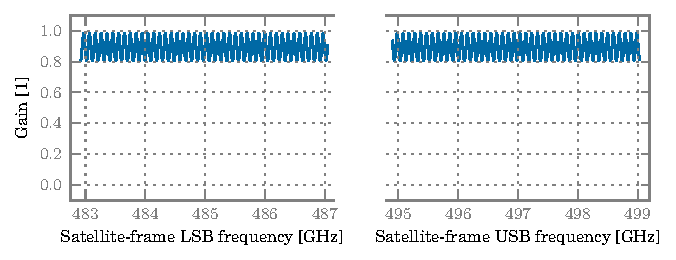
\includegraphics{mars_25_interf_dsb_gain_cold}
    \vspace{-1.1em}
    \caption*{Gain: what the mixer detects if the cold load emits a power of~1.}
    \medskip
    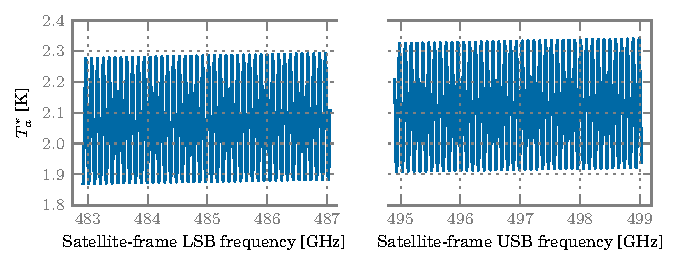
\includegraphics{mars_25_interf_dsb_temp_cold}
    \vspace{-1.1em}
    \caption*{Cold load power seen by the mixer before being folded.}
    \medskip
    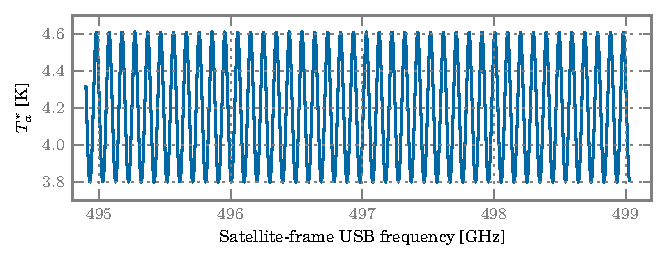
\includegraphics{mars_25_interf_fld_temp_cold}
    \vspace{-1.1em}
    \caption*{Cold load power seen by the mixer after being folded.}
    \medskip
    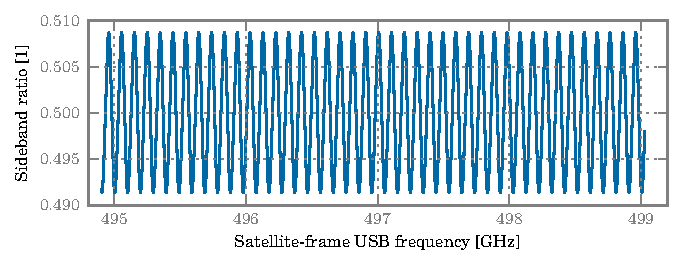
\includegraphics{mars_25_interf_sbr_cold}
    \vspace{-1.1em}
    \caption*{Sideband ratio: USB gain / (LSB gain + USB gain).}
    \caption{Three stages of the interference modeling for the cold load, and the sideband ratio.}
    \label{fig:mars_interf_stages_cold}
\end{figure}
\begin{table}
    \centering
    % HOT
    % ## Distance param 1.6491521148703148
    % ## Distance error 8.5017794640728818e-05
    % ## Angle param 4.1068006437048581
    % ## Angle error 0.08755492869280726
    % X2 = 0.0085045429515
    % COLD
    % ## Distance param 1.5349642234206082
    % ## Distance error 6.4163290218112999e-05
    % ## Angle param 4.1915111156985274
    % ## Angle error 0.068293124275238634
    % X2 = 0.00289102399052
    \begin{tabular}{l c c}
        \toprule
            load
            &
            distance [\si{\meter}]
            &
            argument [\si{\radian}] \\
        \midrule
            hot  & $\num{1.64915} \pm \num{8.5e-5}$    &    $\num{4.11} \pm \num{0.08}$ \\
            cold & $\num{1.53496} \pm \num{6.4e-5}$    &    $\num{4.19} \pm \num{0.06}$ \\
        \bottomrule
    \end{tabular}
    \caption{
        Parameters that make the interference model of the hot and cold spectra fit
        their perfect-sine model.
    }
    \label{tab:interf_vs_perfectsine}
\end{table}
\begin{figure}
    \centering
    \begin{subfigure}{\linewidth}
        \centering
        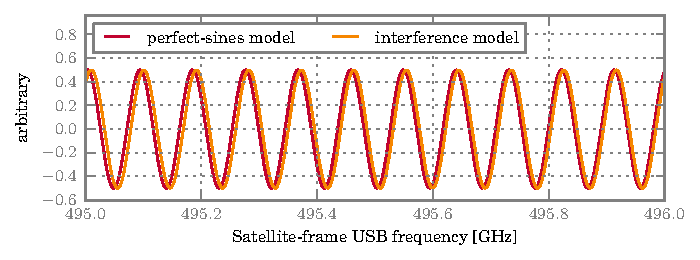
\includegraphics{mars_25_interf_distance_fit_hot}
        \caption{Best fit of the hot ripple.}
        \label{fig:mars_25_interf_distance_fit_hot}
    \end{subfigure}%
    \\
    \begin{subfigure}{\linewidth}
        \centering
        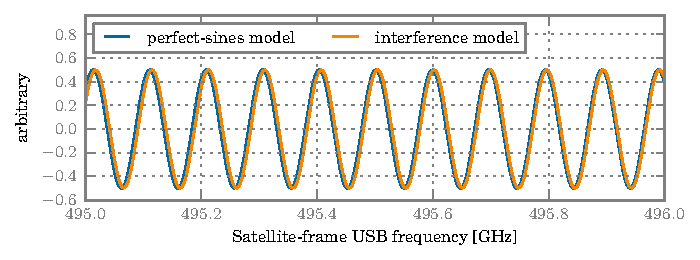
\includegraphics{mars_25_interf_distance_fit_cold}
        \caption{Best fit of the cold ripple.}
        \label{fig:mars_25_interf_distance_fit_cold}
    \end{subfigure}%
    \\
    \begin{subfigure}{\linewidth}
        \centering
        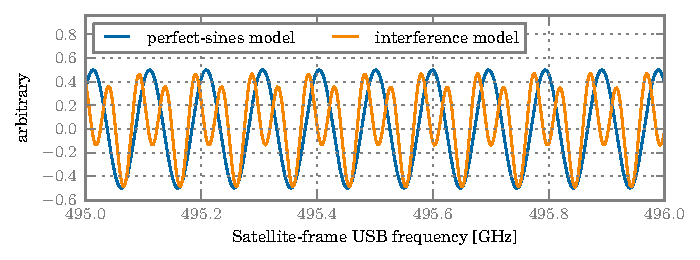
\includegraphics{mars_25_interf_distance_fit_cold_poor}
        \caption{Some narrow ranges of the argument of the reflection coefficient produce complex ripples that prevent a better fit.}
        \label{fig:mars_25_interf_distance_fit_cold_poor}
    \end{subfigure}%
    \caption{
        The period of a ripple relates to the length of a cavity.
        One can determine a cavity length by matching a period 
        (\subref{fig:mars_25_interf_distance_fit_hot} and \subref{fig:mars_25_interf_distance_fit_cold}),
        although complex interference patterns (\subref{fig:mars_25_interf_distance_fit_cold_poor}) make the task difficult.
    }
    \label{fig:mars_25_interf_distance_fit}
\end{figure}


\Cref{tab:interf_vs_perfectsine} lists the parameters of the interference model that best reproduce the perfect-sine model of the hot and the cold load.
The corresponding ripples are shown in~\cref{fig:mars_25_interf_distance_fit_cold,fig:mars_25_interf_distance_fit_hot}.
The vertical axis is arbitrary because the ripples are normalized.
Neither the hot and cold best interference models match the perfect-sine model perfectly.
This is due to the fact that some combinations of distance and argument produce ripples that do not approximate simple sines, as shown in~\cref{fig:mars_25_interf_distance_fit_cold_poor}.



We have compared one model to another in order to determine the mixer--load distances
and the argument of the reflection coefficient of the loads.
This gives us a very good first-guess to seed a fit that compares our complete interference model to the real data from Mars.





%#############################################################################

\section{Full model fit}
The analysis done in the previous section gives us very good first-guesses for the mixer--load distances and the argument of the reflection coefficient of the two loads.
In this section, we compare our interference model to the real Mars data.

The free parameters are
\begin{itemize}[noitemsep,nolistsep]
    \item the hot reflection coefficient, magnitude,
    \item the hot reflection coefficient, argument,
    \item the cold reflection coefficient, magnitude,
    \item the cold reflection coefficient, argument,
    \item the distance between the hot surface and the H mixer,
    \item the distance between the cold surface and the H mixer,
    \item and the physical temperature of Mars.
\end{itemize}

The interference model is compared to the smoothed version of the Mars spectrum, from which the linear trend (first-order polynomial fitted in~\cref{sec:perfect_sines_model}) is removed.
We remove the linear trend because our interference model does not predict it, it may be astronomical and not instrumental in nature.
Without a better model of Mars, we need to leave this trend out.

The result is shown in~\cref{fig:mars_25_interf_smoothed_vs_interf}.
The model parameters for this optimal solutions are listed in~\cref{tab:mars_full_model} for two cases:
in the first case, the coefficient of reflection of the mixer is fixed;
in the second case, it is a free parameter.

The uncertainties given in this table are very conservative estimates:
They are calculated assuming that their probability distribution is Gaussian, which obviously cannot be true for reflection coefficients that must reside inside the complex disk of radius~1.
We include them for the sake of disclosure, but a much better measurement of these uncertainties could be given by Bayesian analysis or Monte Carlo simulations.

\begin{figure}
    \centering
    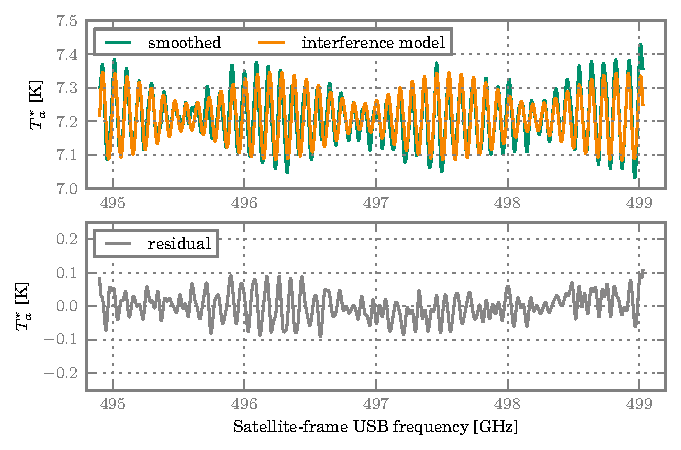
\includegraphics{mars_25_interf_smoothed_vs_interf}
    \caption{Best reproduction of the spectrum of Mars with our interference model.}
    \label{fig:mars_25_interf_smoothed_vs_interf}
\end{figure}

\begin{table}
    % 1.6480265532364544 +/-0.0012526911025520437
    % 1.5339021240876065 +/-0.0010667862540373438
    % 0.037896590464644483 +/-0.23324988755084228
    % 19.392660220711125 +/-31.097964720905996      0.5431042991723657
    % 0.3042926590794563 +/-0.75312073096021415
    % 24.807068124703694 +/-22.943509146023409      2.815919549575141
    % 11.725143032389045 +/-0.15502956205003632
    % STDDEV residual: 0.0380157531167
    \centering
    \begin{tabular}{l r@{}c@{}l r@{}c@{}l l}
        \toprule
        parameter &
        \multicolumn{3}{c}{value} &
        \multicolumn{3}{c}{uncertainty} & unit\\
        \midrule
            hot distance                                 &  1&.&6480  &  0&.&0012 & [\si{\meter}]  \\
            cold distance                                &  1&.&5339  &  0&.&0011 & [\si{\meter}]  \\
            hot reflection coefficient, magnitude        &  0&.&0379  &  0&.&23   & [1]            \\
            hot reflection coefficient, argument         &  0&.&5431  & 31& &     & [\si{\radian}] \\
            cold reflection coefficient, magnitude       &  0&.&3043  &  0&.&75   & [1]            \\
            cold reflection coefficient, argument        &  2&.&8159  & 23& &     & [\si{\radian}] \\
            mars temperature                             & 11&.&72    &  0&.&15   & [\si{\kelvin}] \\
        \bottomrule
    \end{tabular}
    \caption*{Case 1: The magnitude of the reflection coefficient of the mixer is fixed at~$-\sqrt{0.05}$.}
    \bigskip
    \begin{tabular}{l r@{}c@{}l r@{}c@{}l l}
        \toprule
        parameter &
        \multicolumn{3}{c}{value} &
        \multicolumn{3}{c}{uncertainty} & unit\\
        \midrule
            hot distance                                 &  1&.&6480 &  0&.&0012 & [\si{\meter}]  \\
            cold distance                                &  1&.&5339 &  0&.&0011 & [\si{\meter}]  \\
            hot reflection coefficient, magnitude        &  0&.&0442 &  0&.&34   & [1]            \\
            hot reflection coefficient, argument         &  0&.&55   & 31& &     & [\si{\radian}] \\
            cold reflection coefficient, magnitude       &  0&.&7033 &  3&.&07   & [1]            \\
            cold reflection coefficient, argument        &  2&.&40   & 21& &     & [\si{\radian}] \\
            mixer reflection, magnitude                  & -0&.&19   &  1&.&0    & [1]            \\
            mars temperature                             & 11&.&84   &  1&.&32   & [\si{\kelvin}] \\
        \bottomrule
    \end{tabular}
    \caption*{Case 2: The magnitude of the reflection coefficient of the mixer is free.}
    \caption{Interference model parameters that best reproduce the real Mars data.}
    \label{tab:mars_full_model}
\end{table}



%#############################################################################
\FloatBarrier



\section{Discussion}

Although the model seems to fit the data quite well in~\cref{fig:mars_25_interf_smoothed_vs_interf}, the residual shows strong sinusoidal features.
These are due to small mismatches in amplitude or in phase.
This model is not good enough to make quantitative predictions of the ripples, but its qualitative predictions are satisfactory.

For this study, the mixer was modeled as a plane interface with a reflection coefficient whose argument and magnitude do not vary with frequency, which is an extreme simplification of reality (see~\vref{sec:mixer_model}).
The reflection coefficient of a real mixer is frequency-dependent.
This fact alone is sufficient to explain the variable phase difference between our model and the data.
It would be possible to use Tucker's theory of mixing~\parencite{tucker1985quantum} in order to create a more accurate model.

The spectrum of Mars with which we have worked so far is part of a series of spectra taken with different pointings.
\Cref{fig:mars_24_interf_smoothed_vs_interf} shows the very same model applied to another spectrum of Mars.
With this pointing, Mars couples less to the beam, which explains the lower continuum (\SI{4}{\kelvin} here, versus \SI{7.2}{\kelvin} with the original spectrum).
The model shown on \Cref{fig:mars_24_interf_smoothed_vs_interf} results from a fit during which the temperature of Mars is the only free parameter while the other parameters are taken from~\cref{tab:mars_full_model}.
The bandpass of the instrument has not significantly changed between the two pointings, therefore the model fits the new data quite well without modification.

\begin{figure}
    \centering
    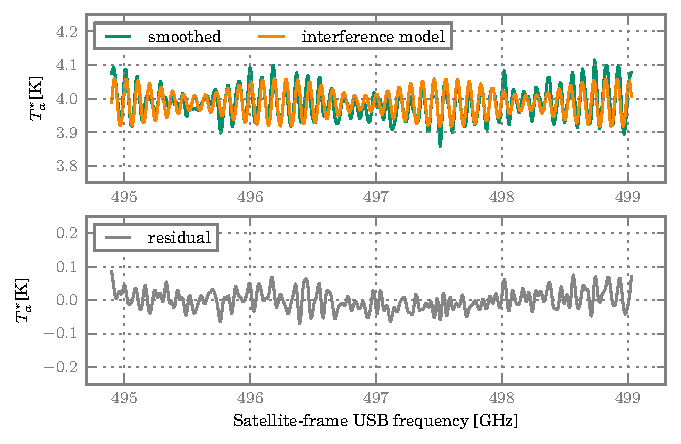
\includegraphics{mars_24_interf_smoothed_vs_interf}
    \caption{Same model applied to another spectrum}
    \label{fig:mars_24_interf_smoothed_vs_interf}
\end{figure}

The magnitude of the reflection coefficients given in~\cref{tab:mars_full_model} may appear surprising.
The calibration loads are supposed to be close to black bodies but the model predicts that the cold load reflects between 30 and \SI{70}{\percent} of the electric field intensity, which corresponds to a reflectivity in power between 10 and \SI{50}{\percent}.
In the next paragraphs we list hypotheses that can explain these surprising results.

The most obvious possible justification is that the data is noisy.
As shown in~\cref{fig:mars_filtered}, the thermal noise is almost as strong as the ripples that we are trying to measure.
We filter some of that noise by cutting the short-periods but that does not remove the contribution of that noise at the periods of our ripples.
The fitter treats that noise as if it were signal and converges toward somewhat incorrect values.

There is a degeneracy between the parameters: one equation for two variables.
Indeed, the behavior of a cavity depends on the product on the reflection coefficient of its two surfaces (see~\vref{eq:fabry_gain_r2_r3}).
For each coefficient of reflection of the mixer, we can find a coefficient of reflection of the hot and cold loads that reproduce the observed ripple: whenever one decreases the other increases to compensate with the same result.
To remove this degeneracy, we need more equations, which means more cavities.
If the LO--mixer cavity were less lossy, it would produce its own ripples and introduce one new equation to the problem, but it would also introduce one additional variable: the reflection coefficient of the LO itself.
This may still help: the load and the LO would form their own cavity (after reflection on the mixer).
With three parameters in three cavities, the degeneracy should disappear.

\begin{figure}
    \centering
    \input{hbb.pdf_tex}
    \caption{Photograph of the hot calibration load of HIFI.}
    \label{fig:hbb_photo}
\end{figure}
The model for the loads may be lacking.
We model the loads as a single plane surface because the Direct Fourier Transform of the HIFI data does not show any evidence of something more complicated.
It may be the case, though, that the loads need to be modeled with two surfaces instead of one, or even as a distributed surface~(see~\vref{sec:distributed_interface}).
The hot load of HIFI is shown in~\cref{fig:hbb_photo}.
It is a wedge-shaped hole coated in an absorbent material.
Although the entire beam is supposed to couple to the wedge-shaped aperture, part of it may couple to the flat surface around it, especially in Band~1 where the beam is the widest.
A better model of the hot load may require two surfaces: one for the aperture and one for its surrounding.
Surprisingly high or low reflection coefficients may result from an inadequate model of the loads.


With more data we could constrain these parameters better and refine the model.
However, even in its current simple state and despite a low signal-to-noise ratio,
the qualitative predictions of the model seem satisfactory.





%#############################################################################
\FloatBarrier



\section{Conclusion}
A physically-based model of the optics of a coherent detector can predict the effects of interferences on the bandpass of that detector.

We created a physically-based model of the optics of HIFI Band~1 and compared its predictions to an actual HIFI observation of the planet Mars.
Despite the low signal-to-noise ratio and a lack of constraints on some parameters of the model, we reproduced the ripples seen on the continuum of the spectrum of Mars.
The amplitudes, frequency and phase of the modeled ripples are very close to the real ones.
Even if we could not constrain our model well enough to achieve a quantitative match in that specific case,
we consider that this is a successful proof of concept for our modeling technique.

We encourage instrument designers to allocate some time to measure the complex reflection coefficients of their optical components for different LO frequencies.
Matching the physically-based model to the real data would allow to correct the calibration by properly taking into account the ripples caused by the interferences in the optics.
%#############################################################################
%\clearpage
%\printbibliography[heading=subbibliography]
%\end{refsection}


\cleardoublepage
\chapter{Astronomy}
\cleardoublepage
%\begin{refsection}
\chapter{Astronomy in presence of interferences}
%\chaptermark{Impact of interferences on S140 data}
\label{sec:chapter5}

%#############################################################################
\section{Introduction}

As discussed in~\cref{sec:chapter1}, when coherent electromagnetic waves superpose they form a resultant wave of greater or lower amplitude.
This phenomenon is called ``interference''.
In~\cref{sec:chapter2}, we developed a model that can predict the impact of interferences on the gain of a coherent instrument.
In~\cref{sec:chapter4}, we modeled the interferences in Band~1 of the Heterodyne Instrument for the Far Infrared (HIFI), which is a double-sideband coherent detector.

In this chapter, we examine how the estimation of astrophysical parameters from submillimeter heterodyne observations is affected by interferences in the instrument.
We attempt to derive the density and the kinetic temperature of a molecular cloud from the intensity ratios of rotational lines of the \ce{CO} molecule.

To assess the effect of interferences on astrophysical results, we have set up a special HIFI observation of the S140 region.
We observed two rotational lines of~\ce{CO} around the source S140~IRS1.
The \transition{CO}{8}{7} spectra were taken with Band~3b and the \transition{CO}{9}{8} spectra with Band~4a.
Each transition was measured with 5 local oscillator frequencies and 19 diplexer settings, for a total of 95 spectra per transition.
These different optical configurations of the instrument modify the electromagnetic interferences.
This modulates the noise and the gain of the instrument and therefore the profile of the lines.

The bandpass calibration of HIFI cannot correct for this effect because it relies on a ``chopper wheel'' method~\parencite{kutner1981recommendations,ossenkopf2002intensity} which introduces even more interferences into the spectra.
As a result, the 95 spectra of \transition{CO}{8}{7} are slightly different from each other, and so are the spectra of \transition{CO}{9}{8}.
This gives 9025 line integrated-intensity ratios.

In order to quantify the relative contributions of the thermal noise and the interferences on the variability of the line ratios, we model the thermal noise seen during these observations and use it to generate synthetic spectra.
These synthetic spectra are affected by the noise but not by the changing optical configuration of the instrument.
The synthetic spectra have their own distribution of line ratios, which we compare to that of the real data.

We use the \radex{} modeling software \parencite{vandertak2007radex}
to recover the densities and kinetic temperatures of the cloud from these line ratios.
The uncertainty on the line ratios translates into uncertainties on the physical parameters of the cloud.



%=============================================================================

\subsection{\texorpdfstring{\ce{CO} as a tracer of \ce{H2}}{CO as a tracer of H2}}

\begin{table}[bp]
    \centering
    \begin{tabular}{l S S c} % S is from SIunitx.
        \toprule
        \multicolumn{1}{c}{transition} &
        % Use multicolumn to protect the header from the influence of S.
        \multicolumn{1}{c}{rest frequency [\si{\giga\hertz}]}
        &
        \multicolumn{1}{c}{$E_\text{up}$ [\si{\kelvin}]}
        &
        \multicolumn{1}{c}{$n_\text{cr}$ at \SI{100}{\kelvin} [\si{\per\centi\meter\cubed}]}
        \\
        \midrule
        \transition{CO}{5}{4}   &  576.2679305 &  82.97 & \num{1.7e5} \\
        \transition{CO}{6}{5}   &  691.4730763 & 116.16 & \num{2.8e5} \\
        \transition{CO}{7}{6}   &  806.6518060 & 154.87 & \num{4.3e5} \\
        \transition{CO}{8}{7}   &  921.7997000 & 199.11 & \num{6.3e5} \\
        \transition{CO}{9}{8}   & 1036.9123930 & 248.88 & \num{8.5e5} \\
        \transition{CO}{10}{9}  & 1151.9854520 & 304.16 & \num{1.1e6} \\
        \transition{CO}{11}{10} & 1267.0144860 & 364.97 & \num{1.4e6} \\
        \transition{CO}{12}{11} & 1381.9951050 & 431.29 & \num{1.8e6} \\
        \transition{CO}{13}{12} & 1496.9229090 & 503.13 & \num{2.1e6} \\
        \transition{CO}{14}{13} & 1611.7935180 & 580.49 & \num{2.6e6} \\
        \transition{CO}{15}{14} & 1726.6025057 & 663.35 & \num{3.0e6} \\
        \transition{CO}{16}{15} & 1841.3455060 & 751.72 & \num{3.5e6} \\
        \bottomrule
    \end{tabular}
    \caption{
        Rest frequencies,
        upper-level energies ($E_\text{up}$)
        and
        critical densities ($n_\text{cr}$) at~\SI{100}{\kelvin}
        of
        the collisional rotation lines of \ce{CO} detectable by HIFI.
        Credit: Leiden Atomic and Molecular Database \parencite{schoier2004leidenmoldb}.
    }
    \label{table:co_transition_frequencies}
\end{table}

In dense ($\ge 10^{4} \: \si{\per\centi\meter\cubed}$) regions of the interstellar medium, the bulk constituent, hydrogen, is in molecular form.
Such regions are therefore often called molecular clouds.
Besides gas, these clouds contain dust grains which,
despite their low abundance (\SI{1}{\percent}) relative to hydrogen,
strongly absorb short-wave (UV, optical, near-IR) light and prevent the observation of embedded stars at these wavelengths.
Longer wavelengths are much less affected, which makes submillimetric spectroscopy a tool of choice to study star formation as it allows to probe deep inside dense clouds.

Unfortunately, the rotational lines of \ce{H2} are in the mid-infrared range, they are dipole-forbidden and have upper-level energies above~\SI{500}{\kelvin}.
This makes \ce{H2} invisible in cold molecular clouds.
However, other less abundant species can interact with \ce{H2} in a measurable way.
This is the case for carbon monoxide, \ce{CO}, which emits rotational lines when it collides with~\ce{H2}.
\Cref{table:co_transition_frequencies} lists the rotational transitions of~\ce{CO} that can be observed by HIFI.

\ce{CO} is the most common molecule in the interstellar medium after~\ce{H2}.
Because its high relative abundance $n_\ce{CO} / n_\ce{H2} \approx 10^{-4}$~\parencite{tielens2005physics} and its stability in molecular clouds, it is considered a tracer of~\ce{H2}.
By measuring~\ce{CO}, we can infer the properties of~\ce{H2} which constitutes most of the cloud.



%=============================================================================
\subsection{S140 IRS1}
\label{sec:s140irs1}
S140 is a high-mass star-forming region in the molecular cloud L1204,
located in the Cepheus constellation at a distance of $746\pm\SI{27}{\parsec}$ \parencite{hirota2008}.

\begin{figure}
    \centering
    \input{12co10.pdf_tex}
    \caption{
        Map of integrated intensity of \transition{CO}{1}{0} around S140~IRS1 taken by the \SI{30}{\meter} telescope of IRAM.
        The equatorial coordinates are given for the mean equinox J2000.
        The black circle in the center represents the position and the half-power beam width (\SI{22}{\arcsec}) of the HIFI beam used in our observation.
        The gray contour follows the ionization front caused by the UV radiation of the B0V star HD~211880 located \SI{7}{\arcmin} south-west of IRS1.
        This star and the two Off positions used for the background calibration are located outside the area covered by this map.
        Map credit: \textcite{koumpia2015}.
    }
    \label{fig:12CO10_moment0}
\end{figure}

The south-western part of S140 is ionized by the ultraviolet radiation of the B0V star HD~211880.
The resulting ionization front is represented on \cref{fig:12CO10_moment0} by the gray line.
It corresponds to a photon-dominated region~\parencite{hollenbach1997dense}, a region in which the temperature and the chemistry of the gas is mainly driven by the UV radiation from the star.
HD~211880 is not visible on the map, it is located~\SI{7}{\arcmin} away from the center.

Deep inside the cloud, shielded from the UV radiation of HD~211880, S140 hosts several infrared sources.
The brightest one IRS1, located at $\alpha = 22^\text{h} 19^\text{m} 18.21^\text{s}$ $\delta = \ang{63;18;46.9}$ (J2000).

S140~IRS is a well-studied object.
It is established that IRS1 is a young stellar object, a newly born massive star of high luminosity ($\SI{8500}{L_\odot}$,~\cite{maud2013s140}).
In addition to the dense gas cloud that still surrounds it, the young star is circled by an accretion disk which is seen almost edge-on.
IRS1 emits two highly-collimated jets of matter in the direction of its axis of rotation, perpendicular to the accretion disk.
The interaction of these jets with the dense interstellar medium produces large scale molecular outflows~\parencite{reipurth2001herbig} which emit in the submillimeter range.
The~\transition{CO}{1}{0} emission of these outflows extends~\SI{30}{\arcsec} in the north-west and south-east directions~\parencite{maud2013s140}.

Although S140 is extended, our observations focus on high-$J$ transitions which require high temperatures in order to be excited (see~\cref{table:co_transition_frequencies}).
We can expect that most of the emission that we detect originates from warm regions of the cloud, close to its core.
The beam size of HIFI is approximately~\SI{22}{\arcsec} at the frequencies of interest,
it covers a radius of~\SI{0.04}{\parsec} at the distance of IRS1.
A PDR model of S140 by \textcite{koumpia2015} predicts that the gas and dust temperatures should be lower than~\SI{100}{\kelvin} at radii greater than \SI{0.0001}{\parsec}: the high-$J$ \ce{CO} core of IRS1 is much smaller than the beam size.
Likewise, the high-$J$ \ce{CO} emission in the outflow extends much less than the \transition{CO}{1}{0} emission, bringing our region of interest well inside our beam size.

Two nearby infrared sources could contaminate our observations.
The luminosity of IRS2 and IRS3 are respectively \SI{2000}{L_\odot} and \SI{1300}{L_\odot}~\parencite{koumpia2015}.
Our beam couples half of the power emitted by IRS3 but IRS3 is~\SI{85}{\percent} less bright than IRS1.
IRS2 is slightly brighter than IRS3 but barely couples to our beam.
Because of their relatively low temperatures and their distance from the center of the beam, we assume that the \transition{CO}{8}{7} and \transition{CO}{9}{8} emission of IRS2 and IRS3 is negligible.

The two emission lines that we are observing allow us to probe the conditions of the gas deep inside the core of IRS1, where the pressure and the temperature are high.
The critical densities given in~\cref{table:co_transition_frequencies} correspond to the volume number density of the molecule that is required for a given energy level to be thermalized.
In first approximation
$n_\text{cr} = A_{j\!\rightarrow\!j'} / k_{j\!\rightarrow\!j'}(T)$
where $A$ is the rate of spontaneous decay (in \si{\per\second})
and $k(T)$ the collisional rate (in~\si{\centi\meter\cubed\per\second})
of the \Jlevel{j}{j'} transition at the temperature~$T$.
We find these parameters in the data files of the Leiden Atomic and Molecular Database \parencite{schoier2004leidenmoldb}.
That database lists different collision rates for the two isomers of~\ce{H2}.
Since they are close, we averaged them.

Our calculation of the critical density underestimates the actual value;
the method presented in \textcite{yang2010} is more accurate
but its results remain of the same order.
Dividing our conservative estimate of $n_\text{cr}=\num{6e5}$
by the relative abundance $n_\ce{CO} / n_\ce{H2} \approx 10^{-4}$,
we find that \transition{CO}{8}{7} is thermalized for $n_\ce{H2} > \SI{6e9}{\per\centi\meter\cubed}$.
\Textcite{poelman2006line} establish that $n_\ce{H2}$ is between \num{e4} and \SI{4e5}{\per\centi\meter\cubed} for S140,
which tells us that our transitions are far from the Local Thermal Equilibrium.



%=============================================================================
\subsection{HIFI, diplexers and interferences}

Our observations of S140 IRS1 used the Bands~3 and 4 of HIFI.
As described in~\vref{sec:diplexer_lo_injection},
Bands~3, 4, 6 and 7 of HIFI use diplexers for their LO-injection.
The purpose of the diplexers is to maximize the coupling of the mixer to both the sky and the LO.
They do so by aligning the polarization of the sky and the LO signals with that of the mixers (see~\cref{fig:diplexer_render}).

Diplexers are interferometers: the optical pathlength difference between two arms determines the output polarization for every frequency.
For each LO frequency, there exist one and only one optimal pathlength difference.
That pathlength difference is achieved by applying an electric current to an actuator, which translates a mirror and changes the length of one arm.
We call this current ``diplexer actuator current'' (DAC) or simply ``diplexer setting'' in the rest of this chapter.

A side-effect of moving the diplexer is that it changes the lengths of optical cavities in the receiver.
This modifies the interferences, which modify the gain of the instrument.

Another way of modifying the interferences in the instrument is to observe at a different LO frequency.
First, each LO frequency requires its own settings for the diodes and multipliers: the reflection coeffient of the LO changes.
Second, each LO frequency pumps the mixer differently, its reflection coefficient also changes.
Third, the mixing process folds the lower and upper sideband on top of each other, making their interferences modulation interfere together.
Since each LO frequency couples the mixers to different lower and upper sidebands, this also modifies the gain of the instrument.

The diplexer setting and the LO frequency provide two independent parameters that allow the exploration of the effect of interferences on astronomical data.


%#############################################################################
\FloatBarrier
\section{Observation}

We scheduled two observations of S140 IRS1 with HIFI.
They are available in the Herschel Science Archive and can be retrieved with the following observation identifiers (``obsid''):
\begin{itemize}[noitemsep,nolistsep]
    \item \transition{CO}{8}{7}, obsid 0x50015e1d;
    \item \transition{CO}{9}{8}, obsid 0x50015d89.
\end{itemize}

With a rest frequency of~\SI{922}{\giga\hertz}, the line of \transition{CO}{8}{7} falls in HIFI Band~3b.
The line of \transition{CO}{9}{8} is located in Band~4a at~\SI{1037}{\giga\hertz}.

We used a non-standard observing mode based on the standard ``dual beam switch spectral scan'', the latter being described in~\cite{hifiobserversmanual}.

``Dual beam switch'' refers to the choice of the reference source used for subtracting the background radiation: two positions on the sky.
\Cref{tab:on_off_positions} lists the positions of the On and the two Off.
The On position is centered on~IRS1.
The two Off positions are~\SI{3}{\arcmin} away from IRS1 in the north-west and south-east directions.
We assume that there is no \transition{CO}{8}{7} or \transition{CO}{9}{8} emission in the Off positions.
First, these transition have upper-level energies well above the kinetic temperature of the cloud at these positions.
Second, both positions are shielded from the UV radiation emitted by HD~211880 and the three infrared sources.

``Spectral scan'' means that each observation contains spectra taken at different local oscillator frequencies.
Changing the LO frequency is one way to modulate the interferences in HIFI.

The non-standard aspect of our observing mode is that, for each local oscillator frequency, there are 19 different diplexer settings instead of a single one.
This allows us to modulate interferences for a given LO frequency.

\Cref{tab:los_and_dacs} lists the five LO frequencies and the nineteen diplexer actuator currents used for each transition.
Each transition is therefore observed $5 \times 19 = 95$ times.
For each transition, there is a LO frequency and a diplexer setting that match nominally (gray background in \cref{tab:los_and_dacs}).

\begin{table}[b]
%dataset 11
%334.79607197925145  63.3615103585033      22h19m11.05s  63º21'41.43729"
%334.8260678609779   63.31298895703982     22h19m18.26s  63º18'46.76025"
%334.8259243886195   63.31303201092469     22h19m18.22s  63º18'46.91524"
%334.7956101137214   63.361555679611314    22h19m10.95s  63º21'41.60045"
%
%dataset 15
%334.8263617781845   63.31300182715389     22h19m18.32s  63º18'46.80658"
%334.8563340071168   63.26442869962732     22h19m25.52s  63º15'51.94332"
%334.85622353208436  63.26443044144398     22h19m25.49s  63º15'51.94959"
%334.82593558348606  63.312952587111134    22h19m18.22s  63º18'46.62931"
    \centering
    \begin{tabular}{lll}
        \toprule
        pointing  & right ascension & declination \\
        \midrule
        Off left  & $22^\text{h}19^\text{m}11.0^\text{s}$ & \ang{63;21;41.5}\\
        On        & $22^\text{h}19^\text{m}18.2^\text{s}$ & \ang{63;18;46.8}\\
        Off right & $22^\text{h}19^\text{m}25.5^\text{s}$ & \ang{63;15;51.9}\\
        \bottomrule
    \end{tabular}
    \caption{Equatorial coordinates (mean equinox J2000) of the three pointings used in our observations.}
    \label{tab:on_off_positions}
\end{table}

\begin{table}[b]
    \centering
    \begin{tabularx}{\textwidth}{Xrrrrr}
        \toprule
        transition & \multicolumn{5}{c}{LO frequencies [\si{\giga\hertz}]} \\
        \midrule
        \Jlevel{8}{7} &  914.4045 &  914.4225 &  914.4450 &                     914.4630 &  \cellcolor{gray!40}914.4810 \\
        \Jlevel{9}{8} & 1029.4830 & 1029.5010 & 1029.5190 & \cellcolor{gray!40}1029.5415 &                    1029.5595 \\
        \bottomrule
        \toprule
        transition & \multicolumn{5}{c}{horizontal diplexer actuator currents [\si{\milli\ampere}]} \\
        \midrule
        \multirow{4}{*}{\Jlevel{8}{7}}
        & 0.503 & 0.499 & 0.493 & 0.488 & 0.481 \\
        & 0.476 & 0.471 & 0.465 & 0.458 & 0.453 \\
        & 0.447 & \cellcolor{gray!40}0.442 & 0.435 & 0.430 & 0.425 \\
        & 0.419 & 0.412 & 0.407 & 0.401 & \\
        \midrule
        \multirow{4}{*}{\Jlevel{9}{8}}
        & 1.336 & 1.332 & 1.325 & 1.318 & 1.313 \\
        & 1.306 & 1.300 & 1.293 & 1.288 & 1.281 \\
        & \cellcolor{gray!40}1.275 & 1.269 & 1.263 & 1.256 & 1.251 \\
        & 1.244 & 1.237 & 1.232 & 1.225 & \\
        \bottomrule
    \end{tabularx}
    \caption{
        Local oscillator frequencies and diplexer actuator currents used for each \ce{CO} transition.
        For each LO frequency there exist an optimal diplexer current;
        in our observation, the LO and diplexer are often mismatched.
        The cells in gray indicate the values that are the closest to an ideal match.
    }
    \label{tab:los_and_dacs}
\end{table}

The 19 diplexer settings create optical pathlength differences in the interferometer of $\pm1~\text{wavelength}$ around the nominal value.

The 5 LO frequencies are very close to each other.
They are separated by only \num{18.0} or \SI{22.5}{\megahertz}
which corresponds to the granularity of the tunable LO frequencies.
For each transition, the LO frequencies cover a range of~\SI{76.5}{\megahertz}.
We have chosen this range in order to sample the interferences created by the mixer--LO, mixer--hot-load and mixer--cold-load cavities.
These cavities introduce periodic modulations of the gain, with periods between~\num{90} and \SI{100}{\mega\hertz} (see~\cref{sec:chapter4}).

The LO frequencies are chosen so that the lines always appear in the upper sideband.
Furthermore, the lines are not placed in the center of the spectra but close to the edge, where the effect of the interferences is stronger (a side-effect of diplexers shown later in this chapter).

A hot-cold measurement is taken for each instrumental configuration: each spectrum is calibrated with its own bandpass, measured with the corresponding LO frequency and diplexer actuator current.




%#############################################################################
\FloatBarrier
\section{Expectations from interference modeling}
\label{sec:s141_interf}
In~\cref{sec:chapter2} we present a technique to model and predict interferences in a coherent optical receiver.
In this section, we apply this technique to the system of networks shown in~\cref{fig:band45_networks}, which models the optics of the HIFI Bands~3 and~4.
This system is made of 23~networks and 48 3D~ports for a given pointing (either sky, hot or cold).
Despite the high numbers, the technique for solving the interferences between each port of each network along every possible optical path is exactly the same as the one solving the very simple 3-networks system of~\vref{fig:implementation_0}.

\begin{figure}[b]
    \centering
    \input{band45_networks.pdf_tex}
    \caption{Networks used to model the interferences in HIFI Bands~3 and~4.}
    \label{fig:band45_networks}
\end{figure}

Even though we focus our study on the output of the H~mixer only, we include the V~mixer and the V~diplexer unit in our model.
This allows taking into account the reflections between both mixers, referred to as ``cross-talk'' by the HIFI calibration team, the effect of which is not always negligible.

We run about \num{36e6} simulations of the gain of the optics from the point of view of the H~mixer: two inputs (LO noise and the source signal) times two polarizations (H and V) times three pointings (sky, cold and hot) times 190 LO and diplexer settings, times the \num{16000} LSB and USB frequencies that correspond to the 8000 channels of a spectrum.
This provides a first impression of the effect of interferences on the gain of the system, and ultimately on the line profile.

\begin{figure}[p]
    \centering
    \begin{subfigure}[b]{\textwidth}
        \centering
        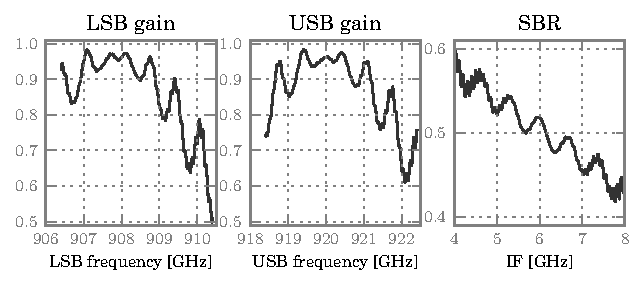
\includegraphics[scale=.9]{87_00_00_sky_s_lsbusbsbr}
        \vspace{-.8em}
        \caption{Sky signal.}
    \end{subfigure}
    \begin{subfigure}[b]{\textwidth}
        \centering
        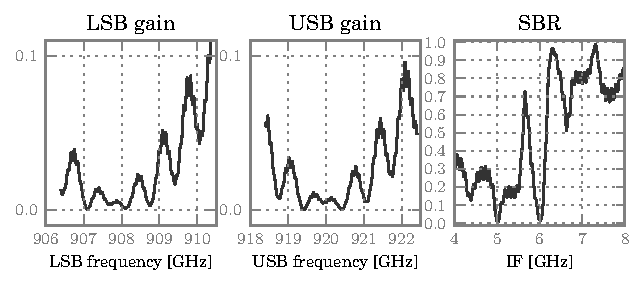
\includegraphics[scale=.9]{87_00_00_sky_l_lsbusbsbr}
        \vspace{-.8em}
        \caption{Sky local oscillator.}
    \end{subfigure}
    \begin{subfigure}[b]{\textwidth}
        \centering
        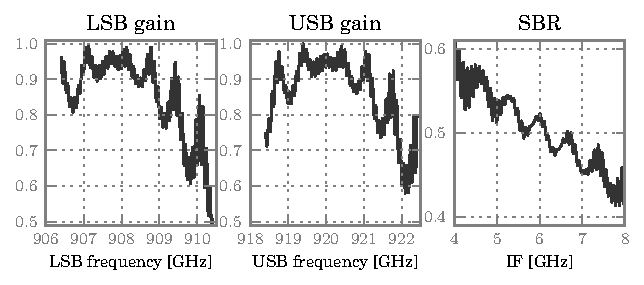
\includegraphics[scale=.9]{87_00_00_hbb_s_lsbusbsbr}
        \vspace{-.8em}
        \caption{Hot load signal.}
    \end{subfigure}
    \begin{subfigure}[b]{\textwidth}
        \centering
        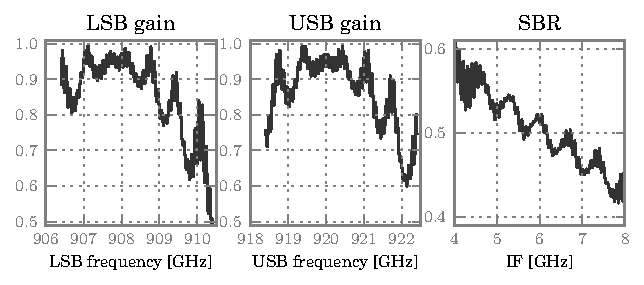
\includegraphics[scale=.9]{87_00_00_cbb_s_lsbusbsbr}
        \vspace{-.8em}
        \caption{Cold load signal.}
    \end{subfigure}
    \caption{Gain and sideband ratio of the optics for the astronomical signal~(a),
    the local oscillator noise~(b),
    the hot load~(c)
    and the cold load~(d).
    $\text{LO frequency} = \SI{914.404500}{\giga\hertz}$,
    $\text{Diplexer current} = \SI{0.503}{\milli\ampere}$.
    }
    \label{fig:87_00_00_sky_lsbusbsbr}
\end{figure}

\begin{figure}
    \centering
    \includegraphics{87_interf_usG}
    \caption{USB gain for the signal of the sky pointing, for the 95 LO and diplexer settings of the~\transition{CO}{8}{7} observation.
    Top: sorted by LO frequency then diplexer setting.
    Bottom: sorted by diplexer setting then LO frequency.}
    \label{fig:87_interf_usG}
\end{figure}
\begin{figure}
    \centering
    \includegraphics{87_interf_usB}
    \caption{USB gain for the signal of the sky pointing, divided by the bandpass, for the 95 LO and diplexer settings of the~\transition{CO}{8}{7} observation.
    Top: sorted by LO frequency then diplexer setting.
    Bottom: sorted by diplexer setting then LO frequency.}
    \label{fig:87_interf_usB}
\end{figure}

\Cref{fig:87_00_00_sky_lsbusbsbr} shows the simulated optical gain for the first spectrum of \transition{CO}{8}{7} when the chopper is pointed at the sky.
With this optical configuration, the mixer detects between~\SI{50}{\percent} and~\SI{100}{\percent} of the power of the astronomical signal and up to~\SI{10}{\percent} of the local oscillator noise.
These curves present several interesting features.
\begin{itemize}[noitemsep,nolistsep]
    \item The widest feature is a bell-shaped (or U-shaped for the LO) curve that spans the entire bandwidth.  It is a product of the diplexer.  Even a perfect diplexer performs optimally at a single frequency.  Its gain degrades as we move away from this frequency and the diplexer starts coupling the mixer to the local oscillator instead.
    \item A ripple of period~$\approx \SI{650}{\mega\hertz}$.
    This matches the length of the cavities formed by the mixers and the rooftop mirrors.
    This is caused by imperfections in the grids (they leak power to the `wrong' polarization) and the rooftop mirrors (a small fraction of the incoming power is reflected without its polarization being rotated).
    \item A ripple of period~$\approx \SI{100}{\mega\hertz}$ that is stronger at the edge of the spectrum and weaker at the center.
    This ripple is caused by the LO--mixer cavity and is modulated by the LO coupling of the diplexer.
    \item A slope in the sideband ratio, which reveals a non-optimal diplexer tuning.
\end{itemize}

The USB gain of the signal for the sky pointing (center top plot of~\cref{fig:87_00_00_sky_lsbusbsbr}) is displayed on \cref{fig:87_interf_usG} for the 95 LO and diplexer settings of the \transition{CO}{8}{7} observation.
This illustrates the influence of the LO and diplexer setting on the intensity and the phase of the ripples affecting the line, which is located at~$\approx \SI{921.8}{\giga\hertz}$.

When the chopper points to the hot or cold calibration load, the non-zero reflectivity of this load introduces more cavities in the system, which creates additional ripples to the gain curves as shown in~\cref{fig:87_00_00_sky_lsbusbsbr} (c) and (d).
The lengths of the mixer--LO, mixer--hot-load and mixer--cold-load cavities are all close to~\SI{1.5}{\meter}, and therefore all produce ripples with periods between~\num{90} and \SI{100}{\mega\hertz}.

The bandpass calibration of HIFI involves dividing the signal measured on the sky by the signal measured on the calibration loads.
The USB gain of the sky signal divided by the bandpass, as measured on the hot and cold loads, is shown in~\cref{fig:87_interf_usB}.
The comparison of~\cref{fig:87_interf_usG} and~\cref{fig:87_interf_usB} clarifies the effect of the bandpass calibration: the bell-shaped curve caused by the diplexer (red region in the center of~\cref{fig:87_interf_usG}) is canceled by the bandpass division.
In reality, the bandpass corrects more than the variable optical gain, it also corrects the frequency-dependent gain of the IF chain (the electronics between the mixer and the detector).
The cost of the bandpass calibration is the injection into the spectrum of the ripples created by interferences in the mixer--load cavities.

In order to produce these models, we have to assume values for the coefficients of reflection of the various networks of the system.
In particular, we set the reflectivity of the calibration loads to~\SI{1}{\percent} in power and that of the LO to~\SI{5}{\percent}.
The mixer reflectivity depends on the polarization: it is low in the polarization that it couples but high in the other; we choose \SI{1}{\percent} and \SI{100}{\percent}.
The wires of the grids have a radius of~\SI{1}{\micro\meter} and are separated (axis-to-axis) by~\SI{4}{\micro\meter}; their conductivity is set to~\SI{e7}{\siemens\per\meter}, the order of the conductivity of aluminum.
We assume that~\SI{2}{\percent} of the power incident on the rooftop mirrors is reflected without its polarization rotated.
Finally, we set the LO attenuation to~\SI{-6}{\decibel}.
We choose values that we think are reasonable but we expect that the spectra measured by HIFI can provide constraints on these values.

Several parameters have not been included in our simulation.
In particular, the phase of the reflection coefficients.
The reflection coefficients of the mixers and local oscillator are likely to have an imaginary part which may depend on the LO frequency: they are neither perfect conductors not perfect dielectrics.
The electronics of the local oscillator requires different settings for different LO frequencies; which change the properties of the diode on which the electromagnetic wave reflects.
Likewise, each LO setting pumps the mixers with a specific power level and we can expect the surface of a mixer to reflect differently according to its pumping.
If these imaginary parts variy quickly with frequency, then we can expect the phase and the periods of the corresponding ripples to change in accordingly.


%#############################################################################
\FloatBarrier
\section{Data reduction}
\label{sec:s140_data_reduction}
Our study focuses on spectra provided by the WBS-H backend of HIFI: the acousto-optic WideBand Spectrometer sensitive to the horizontal polarization.
The WBS allows us to see the full bandwidth of the mixers while still resolving our lines.
We choose the horizontal polarization because its system temperature is lower: in Bands~3 and 4, the V mixer is slightly under-pumped and therefore less sensitive (see~\cref{tab:chapter5_tsys}).

\begin{table}
    \centering
    \begin{tabular}{ccc}
        \toprule
        LO frequency [\si{\giga\hertz}] &
        $T_\text{sys, H}$ [\si{\kelvin}] &
        $T_\text{sys, V}$ [\si{\kelvin}]\\
        \midrule
        \num{914.46}   &   225   &   275 \\ % Tsys_1342192329 0x50003ac9
        \num{1029.52}  &   325   &   425 \\ % Tsys_1342191601 0x500037f1
        \bottomrule
    \end{tabular}
    \caption{
        System temperatures of the H and V mixers at the LO frequencies of our observation, at the intermediate frequency of our line.
        Source: Herschel Science Archive, calibration observations 0x50003ac9
        and 0x500037f1.
    }
    \label{tab:chapter5_tsys}
\end{table}


%=============================================================================

\subsection{Custom pipeline}

Because the observing mode is not standard, one assumption of the default HIFI data reduction pipeline~\parencite{hifiobserversmanual} is not valid.
It is necessary to rerun the pipeline from Level-0 (raw telemetry) to Level-2 (calibrated spectra) with a custom configuration:
the ``doAverage'' task of the pipeline must be disabled.
Leaving it enabled (the default) averages the spectra taken with different diplexer settings, which is not what we want.



%=============================================================================

\subsection{Temperature scale}
The HIFI pipeline produces spectra with a power scale expressed as an antenna temperature~$T_\text{a}$
(see~\textcite{kutner1981recommendations} for details regarding the various temperature scales used in radioastronomy).
That temperature scale is suitable for extended sources as it assumes that the emission of the source is received not only in the main beam but also in the side lobes.

\begin{figure}
    \centering
    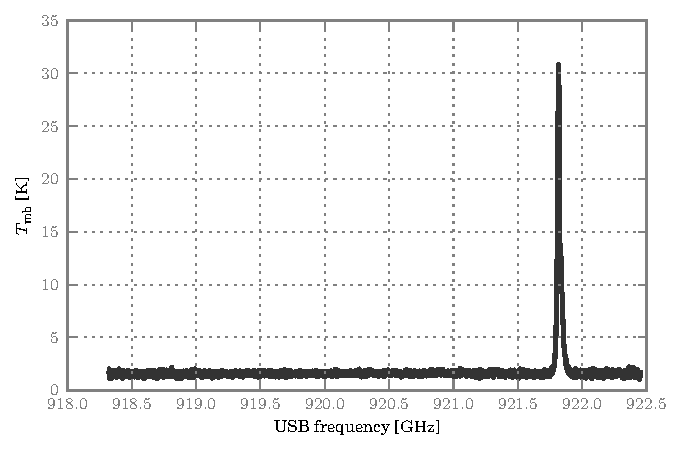
\includegraphics{87_00_00_tmb}
    \caption{
        Spectrum of \transition{CO}{8}{7} shown over its full \SI{4}{\giga\hertz} bandwidth.
    }
    \label{fig:co98_full_bandwidth}
\end{figure}

    % a = 1.22 lambda / D with D = 3.5 and lambda = c_0 / f.
    %   fl =  921.7997000e9 => ll = 0.000325225163341 => al = 0.000113364199793 rad
    %   fu = 1036.9123930e9 => lu = 0.000289120334585 => au = 0.000100779088056 rad
    % To convert to second: sec = 3600*180/pi = 206264.80624709636
    %   al * sec = 23.3830447056765
    %   au * sec = 20.78717907152951
    % To convert to diameter, multiply by distance L = 746 * parsec. (+/-4%)
    % With parsec = 3.086e16 meter
    %   al * L = 2.60982072739e+15 m  (Don't forget, 4% precision)
    %   au * L = 2.32009182242e+15 m
    % Warning, these are diameters.
    % Evgenia uses an inner radius of 2e14 cm = 2e12 m.
    % Her outer radius is 1500 times the inner radius, so 3e15.
    % That does put us pretty much exactly in that area.
    % There, she says that her density gradient for IRS1 goes as r^-0.4, calls it "mild".

Our sources are probably much smaller than our beam size and an absolute calibration of their intensity requires knowing their apparent diameter.
This does not matter for measuring our line ratios:
our two lines originate from the same regions, the ratio cancels their apparent diameter.
For our purpose, the main-beam temperature scale ($T_\text{mb}$) is appropriate.
It assumes that the source fills the main beam but not the sidelobes.

We bring the data to the main-beam temperature scale by dividing our spectra by the main-beam efficiencies $\eta_\text{mb}$ of
\num{0.744} for \transition{CO}{8}{7} and \num{0.740} for \transition{CO}{9}{8}.
We obtain these values by interpolating the beam efficiency tables attached to the HIFI observations for our LO frequencies.
%These tables have a higher granularity that the one presented in fou~\parencite{AA_537_A17}.
\Cref{fig:co98_full_bandwidth} shows one of the 95 spectra of \transition{CO}{8}{7} on the $T_\text{mb}$~scale.
%\begin{equation}
%    T_\text{mb} = T_\text{a}^* / \eta_\text{mb}
%\end{equation}

For both transitions, the \ce{CO} line is always relatively narrow ($\approx \SI{100}{\mega\hertz}$) compared to the instantaneous bandwidth of the instrument (\SI{4}{\giga\hertz}), and in the rest of this chapter we will often zoom in on the line.
The 195 spectra that we study are all very similar to the one shown in~\cref{fig:co98_full_bandwidth}.
The spectra of both transitions typically feature:
\begin{itemize}[noitemsep,nolistsep]
    \item a horizontal baseline of $\SI{1.8}{\kelvin}$ due to the difference of black-body emission at the On and the Off positions in the sky,
    \item a noise of standard deviation $\SI{0.2}{\kelvin}$ slightly stronger at the edges of the spectra than in the center.
    \item an emission line of~$\approx \SI{30}{\kelvin}$ located in the highest-frequency quarter of the spectrum.
\end{itemize}



%=============================================================================

\subsection{Diplexer mis-tuning correction}

%-----------------------------------------------------------------------------
\subsubsection{Motivation}
For our experiment, we use the diplexer as a way of modulating the interferences inside the optics of HIFI.
However, for each LO frequency there exist one and only one diplexer tuning that guarantees ideal couplings and a balanced sideband gain ratio.
By mis-tuning the diplexer, we do modulate the interferences, but we also deteriorate the sideband ratio in a way that is irrelevant for our study.
In this section, we describe how we correct for this degradation of the sideband ratio.

The diplexer units are modules of the HIFI focal plane unit that are used in Bands~3, 4, 6, and 7 for the LO injection~\parencite{jackson2002hifi}.
They are used to align the polarization of the sky and LO signals so that the mixers, which are sensitive to one polarization only, can couple to both optimally.




In normal operations, the diplexer actuator current is adjusted to the LO frequency by interpolation of a look-up table.
For our observations, we bypass this process and set the diplexer actuator current ourselves.
As a result, the diplexer is not optimally tuned.
This is illustrated in~\cref{fig:diplexer_0503}, for which the diplexer actuator current of~\SI{0.503}{\milli\ampere} for a LO frequency of~\SI{914.4045}{\giga\hertz} results in an arm length mis-tuned by \SI{158}{\micro\meter}, approximately half a wavelength.
The coupling is not symmetrical (top plot) and the sideband ratio does not equal \num{0.5} everywhere.
This distorts the line profile.
We must correct for it.

\begin{figure}
    \centering
    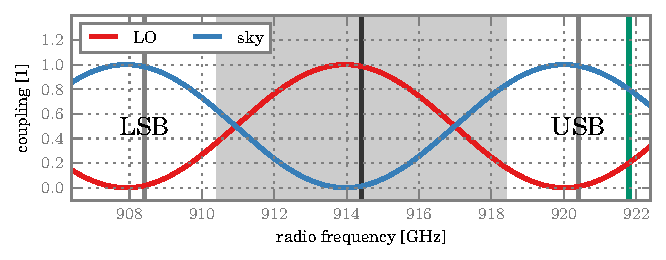
\includegraphics{diplexer_coupling_0503}
    \caption*{
        Coupling of the mixer by the LO and the sky for a mis-tuned diplexer.
        In this specific case, the coupling is shifted \SI{53}{\mega\hertz} to the left of its optimal position.
    }
    \bigskip
    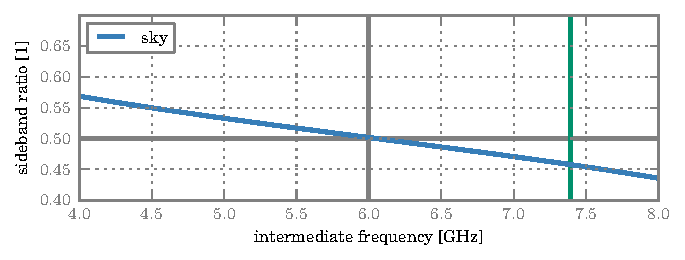
\includegraphics{diplexer_sbr_0503}
    \caption*{
        Sideband ratio of the mixer--sky coupling for a mis-tuned diplexer.
        The left part of the spectrum is USB-dominated, the right part is LSB-dominated.
        The intensity of the \transition{CO}{8}{7} line is underestimated by about~\SI{10}{\percent}.
    }
    \caption{
    Model of the coupling and the sideband ratio for a mis-tuned diplexer.
    The green vertical lines show the rest frequency of the \transition{CO}{8}{7} transition.
    The LO frequency is~\SI{914.4045}{\giga\hertz}.
    The difference in length of the two arms of the diplexer is~\SI{12.3826}{\milli\meter}.
    }
    \label{fig:diplexer_0503}
\end{figure}

%-----------------------------------------------------------------------------
\subsubsection{Correcting for the diplexer mis-tuning}
We start by assuming that the diplexer gain is the same for the four pointings of the observation (Source or On, Reference or Off, Hot, Cold):
$G_L$ for the LSB frequency and $G_U$ for the USB frequency that contribute to the same intermediate frequency.
These gains affect the powers from
the source ($S_L$ and $S_U$),
the reference ($R_L$ and $R_U$),
the hot ($H_L$ and $H_U$) and
the cold ($C_L$ and $C_U$).
The calibration equation of HIFI produces $T_\text{mb}$ from the measured powers, which are distorted by the diplexer:
\begin{equation}
    T_\text{mb}
    =
    \Delta T
    \frac{
        (G_L S_L + G_U S_U) - (G_L R_L + G_U R_U)
    }{
        (G_L H_L + G_U H_U) - (G_L C_L + G_U C_U)
    }\text{.}
\end{equation}
In this equation, $\Delta T$ is a scaling factor converting the dimensionless ratio to a temperature.
Without loss of generality, let us assume $R_L = R_U = 0$: there is no emission from the Off.

%...................................................................
\paragraph{Step 1: find the continuum.}
We assume that parts of the spectrum show only a continuum emission and no line.
Furthermore, we assume that the amplitude of the continuum is constant.
The signal in both sidebands equals this constant: $S_L = S_U = B$.
We get
\begin{equation}
    T_\text{mb}
    =
    \Delta T
    \frac{
        (G_L + G_U) B
    }{
        (G_L H_L + G_U H_U) - (G_L C_L + G_U C_U)
    }
\end{equation}
In this equation, $G_L$ and $G_U$ are known: we calculate them from a known diplexer displacement with~\cref{eq:diplexer_coupling_model}.
We also know $H$ and $C$, the emission from the hot and cold calibration loads: we know their physical temperature $T_h$ and $T_c$, their coupling coefficient and Planck's law.
Finally, $\Delta T = T_h - T_c$ is known as well.
We can therefore easily solve this equation for $B$.
Each channel of the spectrum gives a different value for $B$, but if the spectrum is flat, these values are very close to each other.
We simply take their average.

%...................................................................
\paragraph{Step 2: solve for the line.}
We know that our emission lines are located in the upper sideband.
The lower sideband sees only the continuum.
With $B$ the continuum intensity that we just calculated and $L$ the intensity of the line, we have
\begin{equation}
    T_\text{mb}
    =
    \Delta T
    \frac{
        G_L B + G_U (B + L)
    }{
        (G_L H_L + G_U H_U) - (G_L C_L + G_U C_U)
    }\text{,}
\end{equation}
which we solve for $L$.

Note: this equation cannot make the difference between the noise and the astronomical signal.
Any deviation from the baseline enters~$L$.
The intensity of the noise and the line are both `corrected' equally.

%...................................................................
\paragraph{Step 3: recalibrate.}
The previous steps give us the intensities of the continuum and the line before being distorted by the diplexer mis-tuning.
We can choose whether we re-introduce the continuum or if we leave it out.
The two situations are described by the equations
\begin{align}
    T_\text{mb}'
    &=
    \Delta T
    \frac{B+L}{(H_L + H_U) - (C_L + C_U)} \text{\quad with continuum and}
    \\
    T_\text{mb}''
    &=
    \Delta T
    \frac{L}{(H_L + H_U) - (C_L + C_U)} \text{\quad with the line only.}
\end{align}

In the rest of this chapter, we use the $T_\text{mb}''$ scale.

%-----------------------------------------------------------------------------
\subsubsection{Result of the diplexer mis-tuning correction}
\Cref{fig:diplexer_correction} shows the result of correcting the sideband imbalance with this simple method.
The bottom plot for each transition shows the line only, the continuum is removed.

\begin{figure}
    \centering
    \begin{subfigure}[b]{\textwidth}
        \centering
        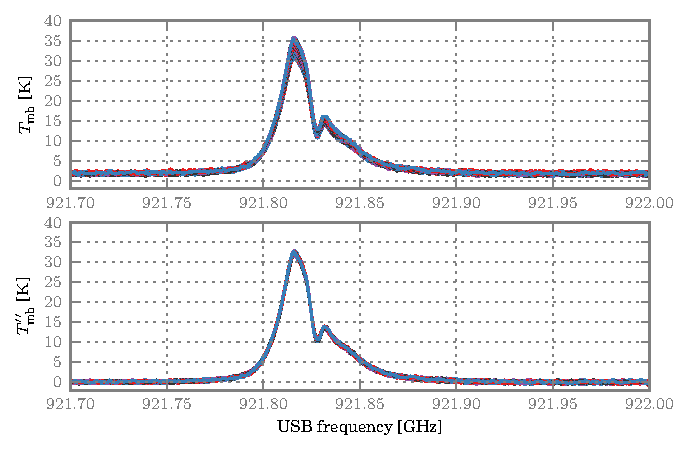
\includegraphics{correction_87}
        \vspace{-.8em}
        \caption{\transition{CO}{8}{7} spectra before and after sideband correction.}
    \end{subfigure}
    \\
    \bigskip
    \begin{subfigure}[b]{\textwidth}
        \centering
        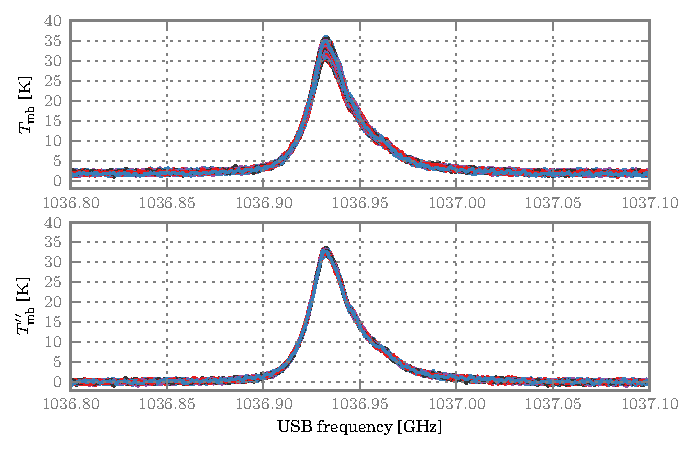
\includegraphics{correction_98}
        \vspace{-.8em}
        \caption{\transition{CO}{9}{8} spectra before and after sideband correction.}
    \end{subfigure}
    \caption{
        Correction of the sideband imbalance due to mis-tuning the mixer.
    }
    \label{fig:diplexer_correction}
\end{figure}


For both transitions, the spread of the peak intensity is considerably reduced.
\begin{table}
    %87 Before correction 31.5146912873 +/- 1.31935031215
    %87 After  correction 32.3597611286 +/- 0.27093631469
    %98 Before correction 31.2396155249 +/- 1.49534099289
    %98 After  correction 32.7454980568 +/- 0.448444802488
    \centering
    \begin{tabular}{ccc}
        \toprule
        transition & before correction & after correction \\
        \midrule
        \transition{CO}{8}{7} & $\num{31.5} \pm \SI{1.3}{\kelvin}$ &
                                $\num{32.4} \pm \SI{0.3}{\kelvin}$\\
        \transition{CO}{9}{8} & $\num{31.2} \pm \SI{1.5}{\kelvin}$ &
                                $\num{32.7} \pm \SI{0.5}{\kelvin}$\\ 
        \bottomrule
    \end{tabular}
    \caption{Peak intensities before and after correcting for the diplexer mis-tuning.}
\end{table}

Any residual spread is due to either thermal noise, imperfections in the diplexers and interferences in the optics.





%#############################################################################
%\FloatBarrier
\section{Noise simulations}
\label{sec:noise_simulations}
We wish to quantify the influence of the thermal noise on the line profiles.
We model the noise seen on HIFI observations and use that model to generate synthetic spectra.
This mimics an observation in which the same source is observed many times with a fixed LO and diplexer settings.
These synthetic spectra differ only by their noise, not by variations in the optical gain.
We proceed in three steps.
First, construct an ideal spectrum for each transition.
Then, model the thermal noise affecting the real spectra.
Finally, apply the modeled thermal noise to the ideal spectra.



%=============================================================================

\subsection{Ideal spectra}
For our ideal hopefully-noiseless spectra, we choose to average the 95~spectra of each transition.
The averaged spectra are shown in~\cref{fig:corrected_averaged}.
We do not claim that these averaged spectra are closer to the astronomical reality than any individual spectrum: averaging reduces the noise but may leave systematic instrumental effects in the bandpass.

By averaging, we reduce the noise by a factor~$\sqrt{95} \approx 10$ but we do not completely eliminate it.

\begin{figure}
    \centering
    \begin{subfigure}[b]{\textwidth}
        \centering
        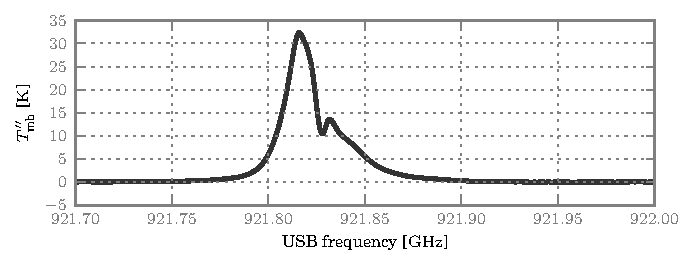
\includegraphics{87_avera_corrected_tmb}
        \vspace{-.8em}
        \caption{Average of the 95 \transition{CO}{8}{7} diplexer-corrected spectra.}
    \end{subfigure}
    \\
    \begin{subfigure}[b]{\textwidth}
        \centering
        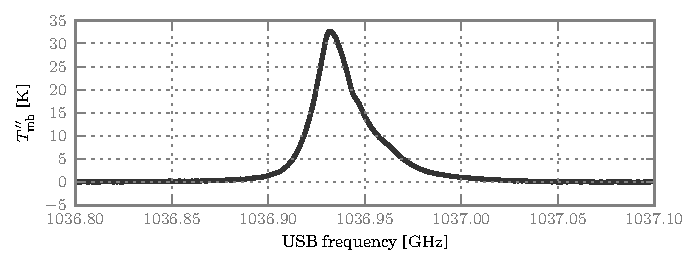
\includegraphics{98_avera_corrected_tmb}
        \vspace{-.8em}
        \caption{Average of the 95 \transition{CO}{9}{8} diplexer-corrected spectra.}
    \end{subfigure}
    \caption{Average of the spectra corrected for diplexer mix-tuning.}
    \label{fig:corrected_averaged}
\end{figure}

%=============================================================================
\subsection{Thermal noise modeling}
We model the thermal noise with a polynomial in Fourier space.

Using Fourier Transforms to analyze a signal is relatively trivial: signals have an analytic expression, they can be written as function of time or frequency.
The noise does not have an analytic expression: it is a stochastic process that can be described only in statistical terms such as variance.
The noise is not visible on the spectra that we measured, what we have is one very specific instance of an inherently random process, one single state taken out of the infinite%
\footnote{Infinite if we assume that the probability distribution is continuous, but quantum processes ultimately limit this to a finite, albeit overwhelmingly large, state space.}
state space of the system.
Fourier analysis treats that particular state as if it were signal.
We must estimate the properties of the stochastic process from that specific sequence.

The power of a stochastic process is, in statistical term, its variance.
The variance can be a function of frequency, for example the ``pink noise'' or the ``$1/f$ noise'' have different variances at different frequencies.
These can be represented on a ``periodogram'', a graph that plots the ``power spectral density'' (PSD) as a function of a frequency/period/scale.
If we consider a time-varying electric potential in volt,
the unit of the PSD of its noise is \si{\volt\squared\second} or \si{\volt\squared\per\hertz}.
In our case, the data is a temperature as a function of frequency;
the PSD of its noise is in~\si{\kelvin\squared\hertz}.
The estimation of the PSD from a signal is a subtle matter, subject of a significant volume of literature (i.e.\ \textcite{burg1967maximum,percival1993spectral}).

In our situation, an accurate estimation of the PSD is not required.
Our goal is to generate 190~synthetic spectra which present 190~particular noise states.
It is sufficient to know these 190~particular states, one does not need to model accurately the entire state space.
We only need the Fourier Transform of our synthetic spectra to match that of the real data.

Taking spectra of spectra can lead to a confusing terminology.
Furthermore there are at least four Fourier spectra of interest for a single direct spectrum.
\Cref{tab:direct_fourier} clarifies the terminology used in this section.

\begin{table}
    \centering
    \begin{tabular}{llcll}
    \toprule
    \multicolumn{5}{l}{Direct spectrum}\\
    \midrule
    $x$-axis & frequency   & $f$ & $\mathbb{R}$ & [\si{\hertz}]\\
    $y$-axis & temperature & $T$ & $\mathbb{R}$ & [\si{\kelvin}]\\
    \bottomrule
    \\
    \toprule
    \multicolumn{5}{l}{Fourier spectra}\\
    \midrule
    $x$-axis & reciprocal frequency & $t$         & $\mathbb{R}$ & [\si{\per\hertz}]\\
    $y$-axis & complex spectrum     & $z$         & $\mathbb{C}$ & [\si{\kelvin}]   \\
             & phase spectrum       & $\arg(z)$   & $\mathbb{R}$ & [\si{\radian}]   \\
             & amplitude spectrum   & $\abs{z}$   & $\mathbb{R}$ & [\si{\kelvin}]   \\
             & normalized-amplitude spectrum & $\abs{z}/n$& $\mathbb{R}$ & [\si{\kelvin}]   \\
    \bottomrule
    \end{tabular}
    \caption{Definitions and units used in Direct and Fourier space.}
    \label{tab:direct_fourier}
\end{table}

Normalized amplitudes allow the comparison of spectra taken with different sampling rates~$\delta f$ and/or different bandwidths~$\Delta f = n \delta f$ (with $n$ the number of channels in the spectrum) by multiplying them by $\delta f / \Delta f = 1/n$.
We use amplitude and normalized-amplitude spectra where necessary:
amplitude spectra can be converted back to direct space;
normalized-amplitude spectra can be compared.

We do not analyze our noise with energy density or power density spectra.
Energy and power density spectra require raising the amplitude to the power 2, which enhances the contrast between the high- and low-amplitude parts of the spectra.
From our experiments, we determined that fitting the energy or power spectrum requires a polynomial of order $>10$ while an order-6 is sufficient to fit the amplitude.
Furthermore, we need our final result in amplitude so that it can be converted back to the direct domain with an inverse-DFT, making the round-trip between amplitude and power unnecessary.

It is easier to measure the noise on the the baseline than on the lines.
The lines are located in the high-frequency half of the direct spectra (see~\cref{fig:co98_full_bandwidth}), therefore we take the Fourier Transform of the lower-frequency half.
We remove any continuum level from the direct spectrum to minimize the artifacts created by the Discrete Fourier Transform (DFT) algorithm.

Finally, we do not apodize our direct spectra with a window.
Windowing is recommended to reduce the ``leakage'' caused by the truncation of the direct data when we need to accurately quantify the amplitude/energy/power at a given frequency on a correct scale.
We are not interested in the absolute levels of amplitude/energy/power;
we are satisfied when the normalized-amplitude of the synthetic spectrum matches that of the real spectrum, leakage included.

%-----------------------------------------------------------------------------
\subsubsection{Noise model of the ideal spectra}

The noise spectra of our ideal spectra are shown in \cref{fig:noise_model_87}(a)
and~\cref{fig:noise_model_98}(a).
The normalized amplitude is in black and its polynomial model in red.

The small plots inside the larger ones zoom into the region in which we expect interferences to leave traces.
Their $x$-axis gives the period of the ripples caused by interferences.
These spectra peak at two periods:
$\approx\SI{90}{\mega\hertz}$ and $\approx\SI{600}{\mega\hertz}$.

The $\SI{90}{\mega\hertz}$ ripple originates from the mixer--LO, mixer--hot-load and/or mixer--cold load cavities.
These cannot be distinguished at this resolution.

The $\SI{600}{\mega\hertz}$ ripple comes from the mixer--rooftop-mirrors cavities.

The averaging process by which we create the ideal spectra retains these two ripples.
This indicates that their phase varies little over the 95~spectra involved in the average:
they interfere constructively.

The polynomial model ignores these peaks of amplitude density: these regions are deliberately masked before fitting the polynomial.
Indeed, the polynomial must follow the thermal noise only and these peaks are not of thermal origin.

%-----------------------------------------------------------------------------
\subsubsection{Noise model of the real spectra}
\label{sec:noise_model_of_the_real_spectra}

The main sources of noise in HIFI are the mixer, the local oscillator and the telescope dish.
The diplexer setting has an influence on how much LO noise the mixer receives but we calculate that our diplexer settings should change that value by less than one percent.
The LO is responsible for less than~\SI{10}{\percent} of the total system temperature.
We conclude that, for modeling our noise, we should not attempt to ``correct'' its intensity for diplexer mis-tuning.
The noise measured on the original spectra is the correct one.

In this step, we do not take the DFT of an average but the average of DFTs.
Indeed, we do not wish to attenuate the noise of the real spectra by averaging them.
However, we wish to reduce the uncertainty of our polynomial model, which we can achieve by averaging the DFTs.

The normalized-amplitude spectra of the baseline, and their polynomial models, are presented in~%
\cref{fig:noise_model_87}(b) and~\cref{fig:noise_model_98}(b).

The two peaks at~\SI{90}{\mega\hertz} and~\SI{600}{\mega\hertz} that are present on the ideal spectra are also visible on these real spectra.
These peaks are less well-defined because the noise is stronger.

A new feature appears on these spectra: a peak at~\SI{875}{\per\giga\hertz} which corresponds to a period of~$\approx\SI{1.14}{\mega\hertz}$.
This peak is visible on the average of DFTs but not on the DFT of averages.
This indicates that the corresponding ripple interferes destructively during the averaging: its phase changes a lot.
It is unlikely that this feature corresponds to a cavity: the cavity would need to be~\SI{130}{\meter}-long.
We have not determined its origin.
Possible explanations include
\begin{itemize}[noitemsep,nolistsep]
    \item An artifact of the sampling of the WBS:
the even and odd channels of the WBS CCD have different levels of dark currents.
These channels are separated by about~\SI{0.5}{\mega\hertz} and an imperfect calibration of these dark currents could generate a~\SI{1}{\mega\hertz}-period ripple.
    \item An artifact of the regridding done by the HIFI pipeline:
the spectra produced by the WBS have an irregular frequency axis.
The pipeline resamples it onto a regular grid.
This might produce some artifacts at the scale of the channel spacing (\SI{0.5}{\mega\hertz}) or the channel resolution~\SI{1.1}{\mega\hertz}.
\end{itemize}
In any case, this feature is non-thermal and its region is masked during the fit of our polynomial model.

\begin{figure}[p]
    \centering
    \begin{subfigure}[b]{\textwidth}
        \centering
        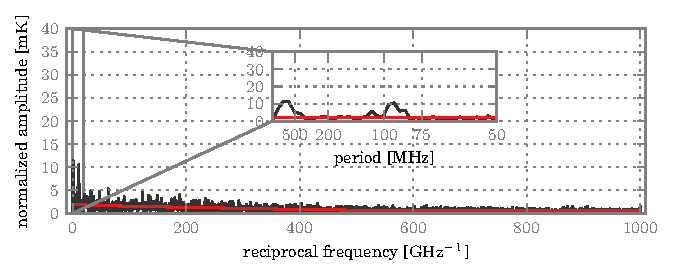
\includegraphics{noise_dft_87_correctedavg}
        \vspace{-.8em}
        \caption{Noise of the average of 95 \transition{CO}{8}{7} diplexer-corrected spectra.}
        %\label{fig:noise_dft_87_correctedavg}
    \end{subfigure}
    \\
    \bigskip
    \begin{subfigure}[b]{\textwidth}
        \centering
        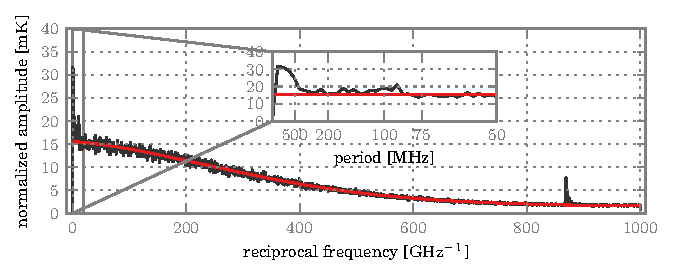
\includegraphics{noise_dft_87_original}
        \vspace{-.8em}
        \caption{Averaged noise of 95 \transition{CO}{8}{7} original spectra.}
        %\label{fig:noise_dft_87_original}
    \end{subfigure}
    \\
    \bigskip
    \begin{subfigure}[b]{\textwidth}
        \centering
        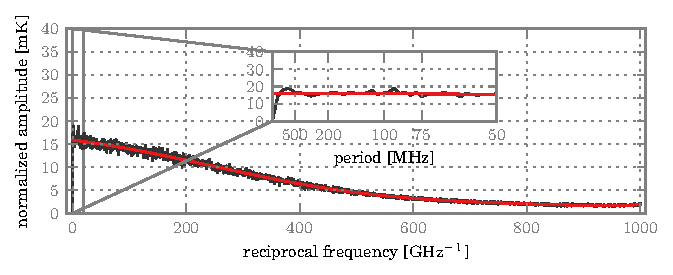
\includegraphics{noise_dft_87_noisy}
        \vspace{-.8em}
        \caption{Averaged noise of 95 \transition{CO}{8}{7} synthetic noisy spectra.}
        %\label{fig:noise_dft_87_noisy}
    \end{subfigure}
    \caption{Noise modeling of the~\transition{CO}{8}{7} spectra.}
    \label{fig:noise_model_87}
\end{figure}

\begin{figure}[p]
    \centering
    \begin{subfigure}[b]{\textwidth}
        \centering
        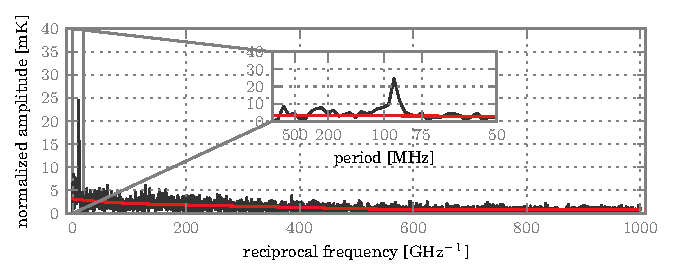
\includegraphics{noise_dft_98_correctedavg}
        \vspace{-.8em}
        \caption{Noise of the average of 95 \transition{CO}{9}{8} diplexer-corrected spectra.}
    \end{subfigure}
    \\
    \bigskip
    \begin{subfigure}[b]{\textwidth}
        \centering
        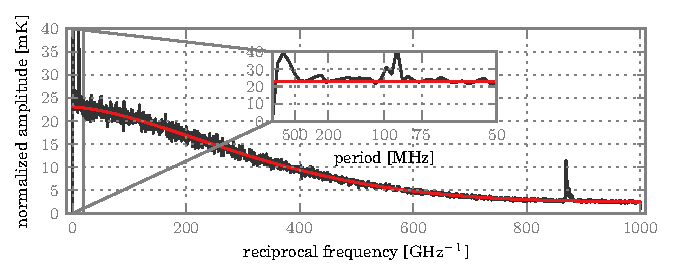
\includegraphics{noise_dft_98_original}
        \vspace{-.8em}
        \caption{Averaged noise of 95 \transition{CO}{9}{8} original spectra.}
    \end{subfigure}
    \\
    \bigskip
    \begin{subfigure}[b]{\textwidth}
        \centering
        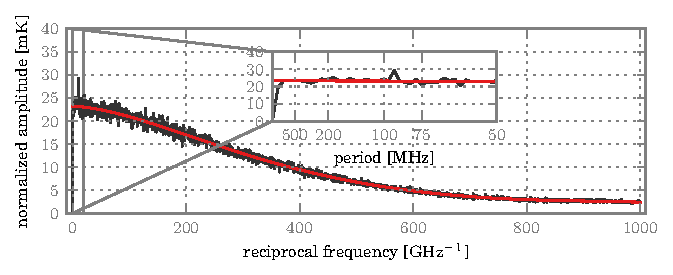
\includegraphics{noise_dft_98_noisy}
        \vspace{-.8em}
        \caption{Averaged noise of 95 \transition{CO}{9}{8} synthetic noisy spectra.}
    \end{subfigure}
    \caption{Noise modeling of the~\transition{CO}{9}{8} spectra.}
    \label{fig:noise_model_98}
\end{figure}


%=============================================================================
\FloatBarrier
\subsection{Synthesis of the thermal noise}
We generate artificial noise in the Fourier space and convert it to Direct space with an inverse Discrete Fourier Transform via a technique called ``phase randomization'' \parencite{yamada1991orthonormal}.

The complex spectrum of our synthetic noise is an array of complex numbers $z=\rho \exp(i \theta)$.
The array $\rho=\abs{z}$ is an amplitude spectrum.
The array $\theta=\arg(z)$ is a phase spectrum.

A polynomial model describes a normalized-amplitude spectrum $\abs{z}/n$ with $n$ the number of channels.
Multiplying that model by the appropriate $n$ gives a amplitude spectrum $\rho$.

We use a pseudo-random number generator with a uniform distribution to generate a phase spectrum with values of $\theta \in [0, 2\pi[$.

We call $A$ the noise model of the ideal spectra and $B$ the noise model of the real spectra.
The noise that we need to add to the ideal spectra in order to bring them to $A$ is not
$C=A-B$: noise adds in power, not in intensity.
The addition in power ($C=\sqrt{A^2-B^2}$) does not produce synthetic spectra with a noise of $A$ either: the randomness is too high (or the number of channels too low).
Instead, we determine $C$ by fitting it; the objective function generates hundreds of synthetic spectra at each iteration until the normalized-amplitude spectrum of their noise matches~$A$.

The average noise of our 190 synthetic spectra (95 per transition) can be seen
in~\cref{fig:noise_model_87}(c) and~\cref{fig:noise_model_98}(c).
As desired, it is very similar to the noise observed on the real spectra (middle plots).
In addition, the peaks present on the top and middle spectra have all but disappeared.

We have created synthetic spectra that mimic the noise seen on the real spectra without including their systematic variability.
We can now analyze the line profiles of the real and synthetic spectra.




%#############################################################################
\FloatBarrier
\section{Line profile analysis}



We begin our analysis by measuring the various components constituting the lines profiles of \transition{CO}{8}{7} and \transition{CO}{9}{8} seen by HIFI in S140 IRS1.

We perform the same analysis with two sets of spectra:
the real HIFI spectra corrected for diplexer-mis-tuning (\cref{sec:s140_data_reduction})
and
the synthetic spectra that simulate an observation that is affected only by thermal noise (\cref{sec:noise_simulations}).


%=============================================================================
\FloatBarrier
\subsection{Gaussian model of the spectra}
\label{sec:chp5_gaussian_model}
\Cref{fig:spectra_transitions} shows the real diplexer-corrected spectra for an arbitrary LO and diplexer setting, one for each transition.
Superimposed on these spectra are the various components of a model.

\begin{figure}
    \centering
    \begin{subfigure}[b]{\textwidth}
        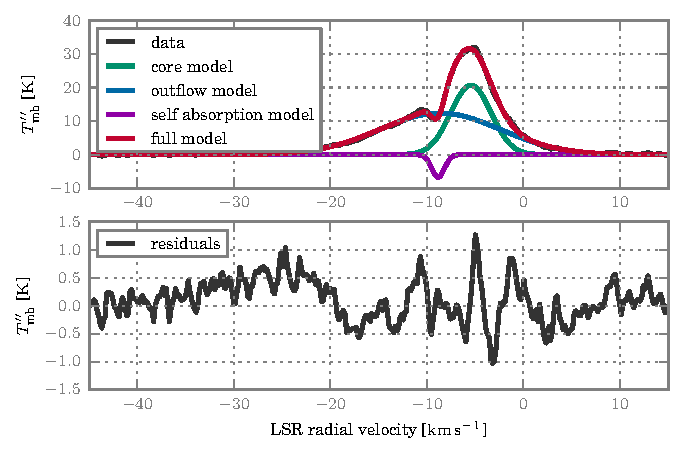
\includegraphics{87_00_00_corrected}
        \vspace{-.8em}
        \caption{\transition{CO}{8}{7}, rest frequency \SI{ 921.7997000}{\giga\hertz}.}
    \end{subfigure}
    \\
    \bigskip
    \begin{subfigure}[b]{\textwidth}
        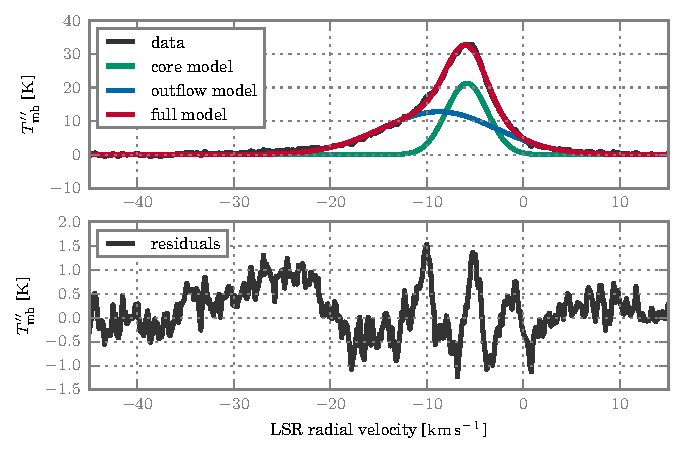
\includegraphics{98_00_00_corrected}
        \vspace{-.8em}
        \caption{\transition{CO}{9}{8}, rest frequency \SI{1036.9123930}{\giga\hertz}.}
    \end{subfigure}
    \caption{
        HIFI WBS-H spectra of S140 IRS1 for \transition{CO}{8}{7} and \transition{CO}{9}{8}.
        For each transition, the the top plot shows the data in black and the model in color, where the full model is the sum of the others; and the bottom plot shows the difference between the data and the full model.
    }
    \label{fig:spectra_transitions}
\end{figure}

The model is composed of three or four elements:
\begin{itemize}[noitemsep,nolistsep]
    \item a constant horizontal continuum ($c$),
    \item a narrow Gaussian for the core emission ($a_0$, $v_0$, $\sigma_0$),
    \item a broad Gaussian for the outflow emission ($a_1$, $v_1$, $\sigma_1$),
    \item and optionally a third negative Gaussian for a self-absorption component
     ($a_2$, $v_2$, $\sigma_2$).
\end{itemize}
Both transitions show a self-absorption, but in the case \transition{CO}{9}{8} the self-absorption is barely visible in the noise, which makes it difficult to fit.
For each Gaussian function, $a$ is the amplitude, $v$ the mean and $\sigma$ the standard deviation.

%-----------------------------------------------------------------------------
\subsubsection{Core and outflow velocity}
The outflow is not as collimated as the jet that creates it; shocks, collisions and turbulence create a wide range of velocities inside the outflow.
In comparison, the velocities in the core are more homogeneous.
Through the Doppler effect, a larger velocity range translates into broader lines, which is why the outflow component (blue in~\cref{fig:spectra_transitions} is wider than the core component (in green).

The \ce{CO} lines of S140~IRS1 are blue-shifted;
the core moves towards us with a radial velocity of~\SI{-5}{\kilo\meter\per\second}.
The peak intensity of the outflow is on the blue side of the core: it approaches us at~\SI{-9}{\kilo\meter\per\second}, faster than the core does.
\Textcite{maud2013s140} measure a speed of~\SI{-25}{\kilo\meter\per\second} for the blue \transition{CO}{1}{0} outflow.
We justify the difference by the distance to the core.
Our high-$J$ lines are emitted near the core, the jet had little time to accelerate the \ce{CO} molecules.
On the other hand, the \transition{CO}{1}{0} outflow is observed much farther and has been accelerated by the jet much longer.

The line profiles do not show any evidence of a bimodal distribution of velocities as one could expect from a rotating disk seen edge-on.
We conclude that the emission that we observe does not originate (solely) from the accretion disk orbitting the young stellar object.

%-----------------------------------------------------------------------------
\subsubsection{Missing red outflow}
Since the outflow of IRS1 is bipolar, one would expect a second outflow line on the red side of the core.
The spectra do not show this second outflow component.
The emission of the red outflow
may be weaker due do different density and temperature conditions
or it may be absorbed by the dense circumstellar envelope before reaching the detector.

%-----------------------------------------------------------------------------
\subsubsection{Self-absorption}
The absorption feature seen at~$v_\text{LSR}=\SI{-9}{\kilo\meter\per\second}$ attests that \transition{CO}{8}{7} is not optically thin at all frequencies.
The absorption and outflow components have a similar velocity:
this is a case of self-absorption, in which the photons at the line wings have a smaller re-absorption probability than the photons at the line center.

%-----------------------------------------------------------------------------
\subsubsection{Structure of the residual}
The difference between the data and our model (``residuals'' on the plots) shows some structure.
In particular, the blue wing of the line is systematically underestimated: the residual at~\SI{-25}{\kilo\meter\per\second} reaches~\SI{0.5}{\kelvin}.
We have attempted to model the outflow with a second Gaussian component in the hope that it would reveal an emission from the red outflow and increase the velocity of the blue one.
These attempts were unsatisfactory: the models converged to an ad-hoc solution that fitted the blue tail with a very wide and flat Gaussian and showed no evidence of emission from the red outflow.

The three peaks in the residual show that Gaussian profiles are not a perfect fit for this spectrum.
This structure may be astronomical or it can be an instrumental artifact.

\begin{figure}[b!]
    \centering
    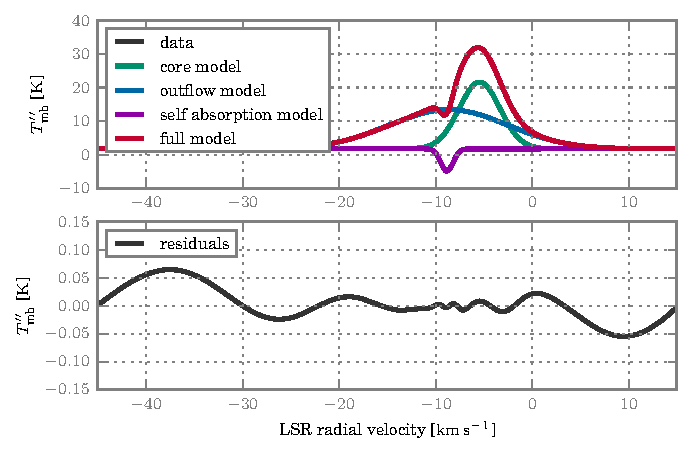
\includegraphics{87_00_00_interf}
    \caption{
        Interference model of HIFI Band~3 applied to a perfectly Gaussian source.
        The interferences introduce ripples the spectrum.
        A Gaussian model of this spectrum leaves a residual that shows some ripples.
    }
    \label{fig:87_00_00_interf}
\end{figure}

We apply the interference model of Band~3 from~\cref{sec:s141_interf} to an input that is made of three perfect Gaussian.
The result is shown in~\cref{fig:87_00_00_interf}.
The interferences modulate the gains and create ripples on the spectrum, which appear on the residual of its Gaussian model.


The small-scale structure located at the frequencies on the line could correspond to that seen on the real spectra, only with a different intensity.
If the real small-scale structure is caused by interferences, then our interference model underestimates them, at least for this specific LO and diplexer setting.

The large-scale structure that modulates the wings of the line does not match that of the real spectra: the interference model creates a long negative red tail that does not exist in the real spectra.
Here, our interference model overestimates the amplitude of that ripple.

It is unlikely that the residual structure is solely caused by interferences in the optics.
Wavelet analysis (\cref{fig:wavelet}) indicates that the periods of the residual structure do not match that of the ripples caused by interferences in known cavities.
They do not match harmonics of these ripples either, harmonics which are anyway unlikely to matter because of the low reflection coefficients in the cavities.
\Cref{fig:wavelet} shows only two scaleograms out of 190.
These scaleograms vary greatly from one spectrum to another.
Most reveal traces of the expected ripple at~\SI{640}{\mega\hertz} that originates from the mixer--rooftop-mirrors cavities, but the indication of a ripple of period between~\num{90} and \SI{100}{\mega\hertz} centered on the line is unclear.

\begin{figure}[p]
    \centering
    \begin{subfigure}[b]{\textwidth}
        \centering
        \includegraphics[width=\textwidth]{50015e1d_WBS-H-USB_04-16_fit_wavelet}
    \end{subfigure}\\
    \begin{subfigure}[b]{\textwidth}
        \centering
        \includegraphics[width=\textwidth]{50015d89_WBS-H-USB_00-12_fit_wavelet}
    \end{subfigure}
    \caption{
        Scaleogram of the continuous wavelet transform
        of the residual of two spectra after subtraction of their Gaussian model.
        The wavelet used is a Morlet wavelet with a time/frequency compromise of 10.
        Colors fade on the edges due to the wavelet sampling 0 outside the defined spectrum.
    }
    \label{fig:wavelet}
\end{figure}

Consequently, we claim that the structure that we observe on the residual of the Gaussian fit of our HIFI spectra is, at least in part, of astronomical nature: the observed emission is not Gaussian.




%-----------------------------------------------------------------------------
\subsubsection{Summary}
The geometry of IRS1 presented by~\textcite{maud2013s140} is that of a source seen almost edge-on: a central object circled by an accretion disk that appears very elliptic (elongated in the NE-SW direction), and two large \transition{CO}{1}{0} outflows perpendicular to the disk (SE is blue-shifted, slightly in front of the core, NE is red-shifted, slightly behind the core).
Our HIFI observation of high-$J$ \ce{CO} lines show a different picture: only the blue outflow is visible as one would expect in the case of a face-on geometry.

Both views can be reconciled if we assume that the system is seen almost edge-on but has a dense circumstellar envelope.
The slight inclination of the polar axis is sufficient to cause the extinction of the red outflow but not that of the blue one, which we would not expect from a homogeneous system.
This suggests a considerable increase of the column density of~\ce{CO} caused by a dense layer of gas between the two outflows, which is compatible with the strong density gradient that we expect close to the central object.
If our high-$J$ \ce{CO} lines originate very close to the center of the system,
the envelope absorbs the emission of the red outflow.

Our lines are not everywhere optically thin, as demonstrated by the visible self-absorption on the blue outflow and the total absence of visible red outflow.
This skews the lines profiles.
Our Gaussian models fit them imperfectly, which can explain the structure of the residual.
In addition, interferences in the optics of the instrument can bring additional distortions to the line profiles.


%=============================================================================
\FloatBarrier
\subsection{Line statistics}
We apply the Gaussian model described in the previous section to the 190 spectra of our observation and the 190 synthetic spectra.
With a least-square Levenberg-Marquardt algorithm, we fit the parameters
$c$,
$a_0$, $v_0$, $\sigma_0$,
$a_1$, $v_1$, $\sigma_1$, and optionally
$a_2$, $v_2$ and $\sigma_2$, for each spectrum independently.

From these fits, we can derive velocity-integrated intensities, then velocity-integrated intensity ratios.

%-----------------------------------------------------------------------------
\subsubsection{Gaussian model parameters}

\Cref{fig:fit_core_87,fig:fit_core_98,fig:fit_outf_87,fig:fit_outf_98,fig:fit_sabs_87,fig:fit_base} present the fitted parameters.
The horizontal axis of each plot corresponds to the spectrum number.
There are 95 spectra for each transition, therefore 95 points on each plot.
The spectra are ordered by LO frequency first (slow-moving index), then by diplexer setting (fast-moving index).

For the Gaussian components, we plot the Full Width at Half Maximum (\textsc{fwhm}) instead of the standard deviation $\sigma$, for its interpretation as a line width is more visual and intuitive; both quantities are linked by
\begin{equation}
    \textsc{fwhm} = 2 \sigma \sqrt{2 \ln(2)}\text{.}    \label{eq:fwhm_sigma}
\end{equation}

The error bars on these plots are fitting errors.
They are calculated by multiplying the diagonal of the covariance matrix by the noise variance (assumed to be that of the baseline) and taking its square root.

When the amplitude and the standard deviation of a Gaussian are known, it is easy to compute the area under that Gaussian, called ``integrated intensity'':
\begin{equation}
    \int_{-\infty}^{+\infty} a \mathrm{e}^{- \frac{(x-v)^2}{2 \sigma^2}}\,\mathrm{d}x
    =
    a \abs{\sigma} \sqrt{2\pi}
    \text{.}
    \label{eq:gaussian_integral}
\end{equation}
We integrate the Gaussian models of the lines over all velocities to produce velocity-integrated intensities in~\si{\kelvin \kilo\meter\per\second}.

The amplitude of the core components for both transitions (\cref{fig:fit_core_87,fig:fit_core_98}) presents some structure:
they cluster around different values for each LO frequency.
The same is true for the amplitude the~\transition{CO}{9}{7} outflow.
The \transition{CO}{8}{7} outflow seems to follow a linear trend, which may be a particular case of the clustering seen on the other plots.
Obviously the LO frequency influences the sideband ratio in ways that our diplexer mis-tuning correction does not predict.
Within a LO frequency, however, the effect of the diplexer is almost drowned in the noise.

In~\cref{sec:s141_interf} we simulated the interferences in optics of HIFI for values that we considered ``reasonable''.
In particular, we used coefficients of reflection that are particularly low: only~\SI{1}{\percent} in power, which means that a single round trip in a cavity results in an attenuation by $0.0001$.
Despite these low reflections, our interference model predicts ripples that are stronger than the ones observed on our data.
Nevertheless, we cannot claim that the reflection coefficients that we used in our model are too high:
when the mixer folds the LSB gain on top of the USB gain, the LSB ripple interferes with the USB ripple (\cref{fig:lo_scan_of_ripple}).
The amplitude and phase of the LSB and USB ripples become degenerated when folded.
Strong ripples can interfere destructively with themselves and weak ripples can interfere constructively.
As a result, we lack constraints to properly model the interferences in the optics of HIFI.



\begin{figure}[b]
    \centering
    \begin{tabular}{@{}c@{}c@{}}
    \toprule
        \multicolumn{2}{c}{\transition{CO}{8}{7} continuum} \\
        diplexer-corrected & synthetic                 \\
    \midrule
        \includegraphics{spread_87_base_ampl_corrected}&
        \includegraphics{spread_87_base_ampl_noisy}        \\
    \bottomrule
    \toprule
        \multicolumn{2}{c}{\transition{CO}{9}{8} continuum} \\
        diplexer-corrected & synthetic                 \\
    \midrule
        \includegraphics{spread_98_base_ampl_corrected}&
        \includegraphics{spread_98_base_ampl_noisy}            \\
    \bottomrule
    \end{tabular}
    \caption{
        Continuum fitted on the real (left) and synthetic (right) spectra for the two transitions.
    }
    \label{fig:fit_base}
\end{figure}

%\afterpage{% Make sure the two figures appear on even/odd pages for comparison.
%    \clearpage% flush all other floats
%    \ifodd\value{page}
%    %\else% uncomment this else to get odd/even instead of even/odd
%        \expandafter\afterpage% put it on the next page if this one is odd
%    \fi
%    {%
    \begin{figure}[p]
        \centering
        \begin{tabular}{@{}c@{}c@{}}
            \toprule
            \multicolumn{2}{c}{\transition{CO}{8}{7} core} \\
            diplexer-corrected & synthetic                 \\
            \midrule
            \includegraphics{spread_87_core_velo_corrected}&
            \includegraphics{spread_87_core_velo_noisy}    \\
            \includegraphics{spread_87_core_vfwh_corrected}&
            \includegraphics{spread_87_core_vfwh_noisy}    \\
            \includegraphics{spread_87_core_ampl_corrected}&
            \includegraphics{spread_87_core_ampl_noisy}    \\
            \includegraphics{spread_87_core_iint_corrected}&
            \includegraphics{spread_87_core_iint_noisy}    \\
            \bottomrule
        \end{tabular}
        \caption{
            Comparison of the \transition{CO}{8}{7} core component parameters
            for the real HIFI data (left column)
            and the synthetic noisy data (right column).
        }
        \label{fig:fit_core_87}
    \end{figure}
%    \clearpage
    \begin{figure}[p]
        \centering
        \begin{tabular}{@{}c@{}c@{}}
            \toprule
            \multicolumn{2}{c}{\transition{CO}{9}{8} core} \\
            diplexer-corrected & synthetic                 \\
            \midrule
            \includegraphics{spread_98_core_velo_corrected}&
            \includegraphics{spread_98_core_velo_noisy}    \\
            \includegraphics{spread_98_core_vfwh_corrected}&
            \includegraphics{spread_98_core_vfwh_noisy}    \\
            \includegraphics{spread_98_core_ampl_corrected}&
            \includegraphics{spread_98_core_ampl_noisy}    \\
            \includegraphics{spread_98_core_iint_corrected}&
            \includegraphics{spread_98_core_iint_noisy}    \\
            \bottomrule
        \end{tabular}
        \caption{
            Comparison of the \transition{CO}{9}{8} core component parameters
            for the real HIFI data (left column)
            and the synthetic noisy data (right column).
    }
        \label{fig:fit_core_98}
    \end{figure}
%    \clearpage
%    }%
%}

%\afterpage{% Make sure the two figures appear on even/odd pages for comparison.
%    \clearpage% flush all other floats
%    \ifodd\value{page}
%    %\else% uncomment this else to get odd/even instead of even/odd
%        \expandafter\afterpage% put it on the next page if this one is odd
%    \fi
%    {%
    \begin{figure}[p]
        \centering
        \begin{tabular}{@{}c@{}c@{}}
            \toprule
            \multicolumn{2}{c}{\transition{CO}{8}{7} outflow} \\
            diplexer-corrected & synthetic                 \\
            \midrule
            \includegraphics{spread_87_outf_velo_corrected}&
            \includegraphics{spread_87_outf_velo_noisy}    \\
            \includegraphics{spread_87_outf_vfwh_corrected}&
            \includegraphics{spread_87_outf_vfwh_noisy}    \\
            \includegraphics{spread_87_outf_ampl_corrected}&
            \includegraphics{spread_87_outf_ampl_noisy}    \\
            \includegraphics{spread_87_outf_iint_corrected}&
            \includegraphics{spread_87_outf_iint_noisy}    \\
            \bottomrule
        \end{tabular}
        \caption{
            Comparison of the \transition{CO}{8}{7} outflow component parameters
            for the real HIFI data (left column)
            and the synthetic noisy data (right column).
        }
        \label{fig:fit_outf_87}
    \end{figure}
%    \clearpage
    \begin{figure}[p]
        \centering
        \begin{tabular}{@{}c@{}c@{}}
            \toprule
            \multicolumn{2}{c}{\transition{CO}{9}{8} outflow} \\
            diplexer-corrected & synthetic                 \\
            \midrule
            \includegraphics{spread_98_outf_velo_corrected}&
            \includegraphics{spread_98_outf_velo_noisy}    \\
            \includegraphics{spread_98_outf_vfwh_corrected}&
            \includegraphics{spread_98_outf_vfwh_noisy}    \\
            \includegraphics{spread_98_outf_ampl_corrected}&
            \includegraphics{spread_98_outf_ampl_noisy}    \\
            \includegraphics{spread_98_outf_iint_corrected}&
            \includegraphics{spread_98_outf_iint_noisy}    \\
            \bottomrule
        \end{tabular}
        \caption{
            Comparison of the \transition{CO}{9}{8} outflow component parameters
            for the real HIFI data (left column)
            and the synthetic noisy data (right column).
        }
        \label{fig:fit_outf_98}
    \end{figure}
%    \clearpage
%    }%
%}

\begin{figure}
    \centering
    \begin{tabular}{@{}c@{}c@{}}
    \toprule
        \multicolumn{2}{c}{\transition{CO}{8}{7} self-absorption} \\
        diplexer-corrected & synthetic                 \\
    \midrule
        \includegraphics{spread_87_sabs_velo_corrected}&
        \includegraphics{spread_87_sabs_velo_noisy}    \\
        \includegraphics{spread_87_sabs_vfwh_corrected}&
        \includegraphics{spread_87_sabs_vfwh_noisy}    \\
        \includegraphics{spread_87_sabs_ampl_corrected}&
        \includegraphics{spread_87_sabs_ampl_noisy}    \\
        \includegraphics{spread_87_sabs_iint_corrected}&
        \includegraphics{spread_87_sabs_iint_noisy}    \\
    \bottomrule
    \end{tabular}
    \caption{
        Comparison of the \transition{CO}{8}{7} self-absorption component parameters for the real HIFI data (left column) and the synthetic noisy data (right column).
    }
    \label{fig:fit_sabs_87}
\end{figure}


%-----------------------------------------------------------------------------
\FloatBarrier
\subsubsection{Velocity-integrated intensity ratio}
\label{sec:line_ratios}
With 95 integrated intensities per transition, there are $95 \times 95 = 9025$ possible line ratios for the core and as many for the outflow.

We calculate the ratio of \transition{CO}{8}{7} over \transition{CO}{9}{8}.
We propagate the uncertainties using
\begin{equation}
    \frac{a \pm \sigma_a}{b \pm \sigma_b}
    =
    \frac{a}{b} \pm \frac{a}{b}\sqrt{(\sigma_a / a)^2 + (\sigma_b / b)^2}
    = c \pm \sigma_c
    \text{.}
\end{equation}
Each possible ratio has a normal distribution $c \pm \sigma_c$.
The sum of these 9025 distributions, divided by the number of distributions, is shown in \cref{fig:ratio_core,fig:ratio_outflow}.
The distribution of this ratio follows a normal curve.
The mean values and their uncertainties are given in \cref{tab:line_ratios}.
The calibration uncertainty is~\SI{4}{\percent} for the core and~\SI{2}{\percent} for the outflow.

The uncertainty on the synthetic ratios is~\SI{60}{\percent} that of the ratios measured on the real HIFI data.
If our noise model is correct, then \SI{40}{\percent} of the uncertainty on the line ratios is caused by non-thermal effects: interferences in the optics, intrinsic sideband ratio of the mixer or the unexplained~\SI{1.14}{\mega\hertz} ripple mentioned in~\cref{sec:noise_model_of_the_real_spectra}.
Longer integration times can reduce the uncertainty due to the noise, but have no effect on the remaining~\SI{2.4}{\percent} of systematic uncertainty on the core line ratio.

\vspace{5em}
\begin{table}[h]
%                        left      right    mean        -         +      fwhm
%    corrected    core   0.9615 .. 1.0546   1.0102   -0.0487   +0.0444   0.0931
%        noisy    core   0.9831 .. 1.0397   1.0113   -0.0282   +0.0285   0.0566
%    corrected outflow   0.9797 .. 1.0266   1.0029   -0.0232   +0.0236   0.0469
%        noisy outflow   0.9859 .. 1.0158   1.0016   -0.0158   +0.0142   0.0299
    \centering
    \begin{tabular}{lcc}
        \toprule
                & diplexer-corrected   & synthetic \\
        \midrule
        core    & $1.01 \pm 0.04$ & $1.01 \pm 0.02$ \\
        outflow & $1.01 \pm 0.02$ & $1.00 \pm 0.01$ \\
        \bottomrule
    \end{tabular}
    \caption{
        Velocity-integrated intensity ratios of
        \transition{CO}{8}{7} over \transition{CO}{9}{8}.
    }
    \label{tab:line_ratios}
\end{table}


\begin{figure}
    \centering
    \begin{subfigure}[0]{\textwidth}
        \centering
        \includegraphics[width=\textwidth]{ratios_core_corrected}
        \caption{Diplexer-corrected spectra;
        $\text{mean}=1.0102$, $\text{FWHM}=0.0931$, $\sigma=0.0395$.}
    \end{subfigure}
    \\
    \begin{subfigure}[0]{\textwidth}
        \centering
        \includegraphics[width=\textwidth]{ratios_core_noisy}
        \caption{Synthetic-noise spectra;
        $\text{mean}=1.0113$, $\text{FWHM}=0.0566$, $\sigma=0.0240$.}
    \end{subfigure}
    \caption{
        Core integrated intensity ratios for the real diplexer-corrected spectra (top)
        and the synthetic spectra (bottom).
    }
    \label{fig:ratio_core}
\end{figure}

\begin{figure}
    \centering
    \begin{subfigure}[0]{\textwidth}
        \centering
        \includegraphics[width=\textwidth]{ratios_outflow_corrected}
        \caption{Diplexer-corrected spectra;
        $\text{mean}=1.0029$, $\text{FWHM}=0.0469$, $\sigma=0.0199$.}
    \end{subfigure}
    \\
    \begin{subfigure}[0]{\textwidth}
        \centering
        \includegraphics[width=\textwidth]{ratios_outflow_noisy}
        \caption{Synthetic-noise spectra;
        $\text{mean}=1.0016$, $\text{FWHM}=0.0299$, $\sigma=0.0127$.}
    \end{subfigure}
    \caption{
        Outflow integrated intensity ratios for the real diplexer-corrected spectra (top)
        and the synthetic spectra (bottom).
    }
    \label{fig:ratio_outflow}
\end{figure}





%#############################################################################
\FloatBarrier
\section{\Radex{} modeling}



%=============================================================================
\subsection{Introduction and parameters}
In the previous section, we have derived the integrated intensity ratio of
\transition{CO}{8}{7} and \transition{CO}{9}{8} of S140~IRS1.
We use the computer program \radex{}%
\footnote{
    \Radex{} is publicly available at the following address:\\
    \url{http://www.sron.rug.nl/~vdtak/radex/index.shtml}.
}
to determine the volume number density and the kinetic temperature of~\ce{H2} from this line ratio.

\Radex{}~\parencite{vandertak2007radex} solves radiative transfer equations for a spherical homogeneous isothermal molecular cloud without large-scale velocity field.
\Radex{} does not assume Local Thermal Equilibrium~(LTE).
The LTE hypothesis states that the excitation temperature $T_\text{ex}$ and the kinetic temperature $T_\text{kin}$ are equal: the energy level population follows the Boltzmann distribution.
The LTE contition is rarely met in the interstellar medium where the densities are low:
the radiative decays compete with collisions and~$T_\text{ex}<T_\text{kin}$, a situation called ``subthermal excitation''~\parencite{vandertak2011radiative}.
For the level population, \radex{} assumes a statistical equilibrium: the sum of the collisional and radiative (de-)excitation rate for each level should be zero.
To solve the radiative transfer, \radex{} uses the escape-probability method first introduced by~\textcite{sobolev1960}.

\Radex{} computes the velocity-integrated intensity of molecular lines resulting from the collisions of a molecule (\ce{CO} for us) with a partner (\ce{H2} in our case).
In addition to tables describing the frequencies, Einstein coefficients, energy levels and collision rates of the molecular transitions, \radex{} requires the line width, the background radiation temperature, the kinetic temperature and volume number density of~\ce{H2}, and the abundance of~\ce{CO} given as a column density.
\Cref{tab:radex_input} lists the input parameters of our model.
\Radex{} calculates the default ortho/para spin ratio of~\ce{H2} by assuming that \transition{H2}{1}{0} is thermalized at the kinetic temperature.

\begin{table}
    \centering
    \begin{tabular}{lrl}
        \toprule
        parameter & value & unit \\
        \midrule
        molecule                         & \ce{^{12}C^{16}O} & \\
        collision partner                & \ce{H2}  & \\
        low frequency                    &  921.78  & \si{\giga\hertz} \\
        high frequency                   & 1036.91  & \si{\giga\hertz} \\
        ortho/para ratio of~\ce{H2}      & default  & \\
        background radiation temperature & 2.73     & \si{\kelvin}                \\
        line width (core)                &  4.98    & \si{\kilo\meter\per\second} \\
        line width (outflow)             & 14.34    & \si{\kilo\meter\per\second} \\
        \ce{H2} volume number density    & $10^{4.5}$ to $10^8$ & \si{\per\centi\meter\cubed} \\
        Kinetic temperature              & \numrange{20}{600}  & \si{\kelvin} \\
        \ce{CO} column density           & $10^{17}$ to $10^{19}$ & \si{\per\centi\meter\squared} \\
        \bottomrule
    \end{tabular}
    \caption{Parameters used in our \radex{} models.}
    \label{tab:radex_input}
\end{table}

For S140, a realistic number column density for \ce{CO} is~\SI{e19}{\per\centi\meter\squared}.
We also explore column densities of \num{e17} and \SI{e18}{\per\centi\meter\squared} which are realistic for \ce{C^{18}O} and \ce{^{13}CO}, respectively.

\Radex{} takes a single line width for the two transitions.
We set it to the average of the two line widths, which is not a problem for the core component but less justified for the outflow where they differ by~\SI{6}{\percent}
(see~\cref{tab:line_widths}).

\begin{table}
    % Linewidth
    % Corrected data:
    %     87 core 4.95989473684 +/- 0.0678930232342
    %     98 core 4.99625263158 +/- 0.0818054133354
    %     87 outf 14.7908421053 +/- 0.152892553658
    %     98 outf 13.8824210526 +/- 0.254130988974
    % Noisy (synthetic noise):
    %     87 core 4.96398947368 +/- 0.049699622944
    %     98 core 4.99835789474 +/- 0.0585537837852
    %     87 outf 14.7727368421 +/- 0.0790262062498
    %     98 outf 13.8842105263 +/- 0.126104208765
    %
    % Error propagation on a sum:
    %     c = a + b
    %     dc = sqrt(da^2+db^2)
    % I use that to compute the average of the linewidths that I can feed to RADEX.
    %
    % Corrected:
    %     avg core  4.97807368421 +/- 0.05315446419364808
    %     avg outf 14.33663157895 +/- 0.1482891537849007
    % Noisy:
    %     avg core  4.98117368421 +/- 0.038401165725599144
    %     avg outf 14.3284736842  +/- 0.0744100341729572
    \centering
    \begin{tabular}{lrrrr}
        \toprule
                & \transition{CO}{8}{7} & \transition{CO}{9}{8} &
                \multicolumn{1}{c}{average} &
                \multicolumn{1}{c}{$\abs{\text{difference}}$} \\
        \midrule
        core    & $ 4.96 \pm 0.07$  & $ 5.00 \pm 0.08$  & $ 4.98 \pm 0.05$ & $0.04 \pm 0.11$\\
        outflow & $14.79 \pm 0.15$  & $13.88 \pm 0.25$  & $14.34 \pm 0.15$ & $0.91 \pm 0.30$\\
        \bottomrule
    \end{tabular}
    \caption{
        Line widths (\textsc{fwhm}) in \si{\kilo\meter\per\second} of the core and outflow components of
        \transition{CO}{8}{7} and \transition{CO}{9}{8}.
    }
    \label{tab:line_widths}
\end{table}



%=============================================================================
\FloatBarrier
\subsection{Results}
\Cref{fig:radex_core,fig:radex_outf} present the line ratios that \radex{} predicts as a function of the temperature and density of~\ce{H2} for several column densities of~{CO}.
The contours follow the mean and the full-width at half-maximum of the line ratio distributions derived in~\cref{sec:line_ratios}:
the outer contours correspond to the total uncertainty and the inner contours to the thermal-noise uncertainty only.

\begin{figure}
    \centering
    \begin{tabular}{cc}
        \toprule
        $N_\ce{CO}$ [\si{\per\centi\meter\squared}]
        &
        core velocity-integrated intensity ratio
        \\
        \midrule
        $10^{17}$ &
        \begin{minipage}{9.5cm}
            \includegraphics[width=\linewidth]{radex_grid_core_n170_t00273}
        \end{minipage}
        \\
        $10^{18}$ &
        \begin{minipage}{9.5cm}
            \includegraphics[width=\linewidth]{radex_grid_core_n180_t00273}
        \end{minipage}
        \\
        $10^{19}$ &
        \begin{minipage}{9.5cm}
            \includegraphics[width=\linewidth]{radex_grid_core_n190_t00273}
        \end{minipage}
        \\
        \bottomrule
    \end{tabular}%
    \caption{\Radex{} predictions of the integrated intensity line ratio \transition{CO}{8}{7}/\transition{CO}{9}{8} in the core of IRS1 as a function of the volume number density of molecular hydrogen and its kinetic temperature, for four column densities of~\ce{CO}.}
    \label{fig:radex_core}
\end{figure}


\begin{figure}
    \centering
    \begin{tabular}{cc}
        \toprule
        $N_\ce{CO}$ [\si{\per\centi\meter\squared}]
        &
        outflow velocity-integrated intensity ratio\\
        \midrule
        $10^{17}$ &
        \begin{minipage}{9.5cm}
            \includegraphics[width=\linewidth]{radex_grid_outf_n170_t00273}
        \end{minipage}
        \\
        $10^{18}$ &
        \begin{minipage}{9.5cm}
            \includegraphics[width=\linewidth]{radex_grid_outf_n180_t00273}
        \end{minipage}
        \\
        $10^{19}$ &
        \begin{minipage}{9.5cm}
            \includegraphics[width=\linewidth]{radex_grid_outf_n190_t00273}
        \end{minipage}
        \\
        \bottomrule
    \end{tabular}%
    \caption{\Radex{} predictions of the integrated intensity line ratio \transition{CO}{8}{7}/\transition{CO}{9}{8} in the outflow of IRS1 as a function of the volume number density of molecular hydrogen and its kinetic temperature, for four column densities of~\ce{CO}.}
    \label{fig:radex_outf}
\end{figure}

In all cases, a line ratio of~\num{1.01} indicates temperatures above~\SI{200}{\kelvin}.
This result could be predicted simply by considering that the upper-level energies
of~\transition{CO}{8}{7} and \transition{CO}{9}{8} are~\SI{200}{\kelvin} and~\SI{250}{\kelvin} (\cref{table:co_transition_frequencies}).
This confirms the assumption that we made in~\cref{sec:s140irs1} regarding the angular size of the emitting region: 
we seem to be probing a warm region of the molecular cloud, a region close to the young stellar object at the center of IRS1.

In addition to a lower-limit on the temperature, these plots give a lower-limit of the density: $n_\ce{H2} > \SI{e5}{\per\centi\meter\cubed}$.
According to~\textcite{goldsmith2001}, at densities above $10^{4.5} \si{\per\centi\meter\cubed}$, the dust and the gas are collisionally coupled.
This suggests that the dust temperature is also of the order of~\SI{200}{\kelvin} in that region, in which case out background temperature of~\SI{273}{\kelvin} may be underestimated.
We have run our \radex{} analysis with background temperatures up to~\SI{100}{\kelvin} and confirmed that the influence of the background temperature on the interpretation of our line ratio is negligible.

For number volume densities of \ce{H2} above~\SI{e6}{\per\centi\meter\cubed}, our line ratio can constitute a useful tracer of temperature.
For low ($<10^{18}$) number column densities of \ce{CO}, the uncertainty on the line ratio translates linearly into an uncertainty on the temperature (although the distribution may be skewed).
However, this same uncertainty makes it absolutely unusable at higher column densities.



%=============================================================================
\FloatBarrier
\subsection{Discussion}

The number column density of~\ce{CO} in the direction of S140 IRS1 has been estimated to~\SI{3e19}{\per\centi\meter\squared}~\parencite{poelman2006line,koumpia2015}.
In this domain, the lines of~\transition{CO}{8}{7} and~\transition{CO}{9}{8} are optically thick, as evidenced by the self-absorption feature observed on the line profile in~\cref{fig:spectra_transitions}.
\Radex{} does not take into account the variation of optical depth along the profile of the line \parencite{langevelde2004} which makes these lines sub-optimal for the study of~S140~IRS1 with \radex{}.
In order to continue their study one should use more detailed models (see \cite{zadelhoff2002} for a list), which often converge much slower.

A recent study \parencite{koumpia2015} using techniques similar to ours (\radex{} modeling of HIFI spectra of \transition{CO}{9}{8}, \transition{C^{18}O}{9}{8} and~\transition{^{13}CO}{10}{9} of S140~IRS1) concludes that the temperature of the gas is approximately~\SI{50}{\kelvin} near the core.
This contrasts with our lower-limit estimate of~\SI{200}{\kelvin}.
One explanation for this discrepancy is that this study involves low-$J$ \ce{CO} lines: the kinetic temperature of~\SI{50}{\kelvin} is derived from the ratios of~\transition{CO}{1}{0} and~\transition{CO}{2}{1}, and the higher-$J$ data provides additional constraints.
With upper-energy levels of~\num{5.53} and~\SI{16.6}{\kelvin}, \transition{CO}{1}{0} and~\transition{CO}{2}{1} are visible in cold regions of the cloud, far away from its hot central object, their emission fills the beam.
Combining high and low-$J$ transitions without modeling the temperature gradient can result in a slightly over-estimated large-scale temperature (a minor concern for their study) or a greatly under-estimated temperature of the small-scale core.

If we compare our observation to the PDR model presented in the same article (spherical PDR, inner-radius $n_\ce{H2}=\SI{e5}{\per\centi\meter\cubed}$, radiation of~100~Drain fields), we find that our temperature of~\SI{200}{\kelvin} originates within~\SI{20}{\astronomicalunit} of the central star.
This places us near the inner radius of the accretion disk~\parencite{maud2013resolving}.

More detailed PDR models can take into account the clumpy nature of S140 reported by~\textcite{poelman2006line}.
This is a refinement over the simple gradient of temperature: there are regions of lower density which allow the UV radiation to penetrate farther into the molecular cloud, creating hotter regions at a greater distance from the core.

An alternative to complex models is to keep using \radex{} with other transition lines.
Isotopes of~\ce{CO} such as \ce{^{13}CO} or \ce{C^{18}O} are less abundant than \ce{CO}.
Consequently their lines can remain optically thin even at high column densities, allowing~\radex{} to perform more optimally.
However, a lower abundance also implies a lower signal-to-noise ratio and therefore a longer integration time.
That longer integration time would certainly lower the noise but would have no effect on the modulation of the optical gain of the detector by interferences; one would trade a well known uncertainty for another, much more difficult to handle.


%#############################################################################
\FloatBarrier
\section{Conclusion}
We observed S140 IRS1 with HIFI and measured the intensities of its~\transition{CO}{8}{7} and \transition{CO}{9}{8} lines.
The line profiles show evidence two sources of emission:
a core and an outflow.

Each line was observed 95 times, with 95 different optical configurations of HIFI.
The optical configuration influences the line profiles.
A statistical analysis of these 190 spectra allowed us to compute the uncertainties on the line velocity-integrated intensity ratios of \transition{CO}{8}{7} over \transition{CO}{9}{8}.
The ratio is $1.01 \pm 0.04$ for the core and $1.01 \pm 0.02$ for the outflow.

In order to quantify the uncertainties due to the thermal noise and that due to non-thermal effects such as interferences in the optical cavities of HIFI, we modeled the thermal noise and created synthetic spectra.
The line ratios measured on these synthetic spectra have a smaller uncertainty than the line ratios measured on the real spectra.
In our study, only \SI{60}{\percent} of the uncertainty on the line ratio is due to thermal effects; the remaining \SI{40}{\percent} have a systematic origin.
The systematic uncertainty on our line ratios is~\SI{2.4}{\percent}.

Sources of systematic uncertainties include
interferences in the optics,
an intrinsic sideband gain imbalance of the mixer
and an unexplained~\SI{1.4}{\mega\hertz} oscillation of the baseline.
We lacked the signal-to-noise, the spectral resolution and the number of equations to properly constrain the many free parameters of an interference model of HIFI.
Nevertheless, we have shown that even low coefficients of reflection are sufficient to explain all the systematic uncertainty that we observed.

The lines that we observed are narrow ($< \SI{100}{\mega\hertz}$), of the order of the period of the shortest ripple ($\approx~\SI{90}{\mega\hertz}$) caused by interferences in HIFI.
In consequence, the ripples are almost undetectable on these spectra, they do not create clear sinusoidal distortions of the line profile, they merely shift the amplitude or velocity of the line.
The continuum being low, its modulation by interferences is drown in the noise.
Consequently, the spectra show no obvious evidence of being affected by interferences
and the astronomer could be mislead into trusting the measurement beyond the irreducible~\SI{2.4}{\percent} of accuracy.

We used \radex{} to predict the line ratios that we expect from a molecular cloud as a function of its density, kinetic temperature and \ce{CO} abundance.
In the specific case of S140 IRS1, the lines of \transition{CO}{8}{7} and \transition{CO}{9}{8} are optically thick, which makes this line ratio useless as a tracer of temperature or density.
However, if the column density of \ce{CO} were lower, the uncertainty on the line ratio would translate almost linearly into an uncertainty on the gas kinetic temperature.

Despite these uncertainties, we estimate that the emission of \transition{CO}{8}{7} and \transition{CO}{9}{8} in S140 IRS1 originates from a warm ($T_\text{kin}> \SI{200}{\kelvin}$) and dense ($n_\ce{H2} > \SI{e5}{\per\centi\meter\cubed}$) region,
possibly within~\SI{20}{\astronomicalunit} of the young stellar object if we neglect the clumpiness of the cloud, but not from the accretion disk itself.


%#############################################################################
\section*{Acknowledgements}
I would like to thank my many supervisors for their suggestions, support and feedback during the writing of this chapter.
In no particular order:
John Pearson, who suggested using S140 to constrain the imaginary part of the reflection coefficients in the HIFI FPU;
Floris van der Tak, whose familiarity with S140 and \radex{} made him indispensable all along;
Marc Verheijen, whose astronomical expertise is related but different, allowing him to evaluate my work from a more objective point of view;
and finally Peter Roelfsema, who on many occasion helped me bridge the gap between engineering and astronomy.

In addition, I especially wish to express my gratitude to David Teyssier, who wrote the non-standard observing mode that we use in our observations;
to Ian Avruch, who worked under a high time pressure to set up the specific observation parameters and submit them to the Mission Operation Center for the last calibration campaign of the HIFI mission;
and to Evgenia Koumpia, for her expertise of S140 which kept my data analysis on the right track.
%#############################################################################
%\clearpage
%\printbibliography[heading=subbibliography]
%\end{refsection}


\begin{appendices}
\chapter{Diplexer}
\chapter{Diplexer}
\label[appendix]{sec:annex_a}


\begin{figure}[b]
    \centering
    \includegraphics[width=\textwidth]{rooftop_polar_lowres}
    \caption{Rooftop mirrors flip the direction of one polarization and keep the other constant.}
    \label{fig:rooftop_polar}
\end{figure}

\begin{figure}[b]
    \centering
    \input{diplexer.pdf_tex}
    \caption{Principle of the Martin--Puplett interferometers used in HIFI Bands~3, 4, 6 and 7.}
    \label{fig:diplexer}
\end{figure}

The diplexer units of HIFI contain a Martin--Puplett interferometer~\parencite{martin1982polarizing} composed of one wire-grid polarizer and two rooftop mirrors.
\Cref{fig:diplexer} illustrates its principle.
The input wave (sky or LO, purple on the figure) is split in two by the wire grid polarizer.
Each half (blue and red) carries one half of the power and travels down one arm of the interferometer where it eventually meets a rooftop mirror.
The rooftop mirrors are oriented so that the input waves are reflected back toward the grid with their polarization rotated by~\SI{90}{\degree}: if the first encounter with the grid is reflective then the second is transmissive and vice versa.
The two waves propagating toward the mixer can be seen as a single output wave (principle of superposition).
The phase difference between the two waves determines the polarization of that output wave.
On the figure, the dots on the paths of the wave represent the crests of that wave;
we can see that the blue and red dots are not in phase when they reach the mixer.
The phase difference depends on the the length of the mobile arm (red) and the frequency of the wave.

An ideal diplexer is modeled by
\begin{align}
    G_\text{sky}(f)
    &=
    \cos
    \left(
        2 \pi
        \frac{df}{c}
    \right)^2
    \\
    G_\text{LO}(f)
    &=
    1 - G_\text{sky}(f)
    \label{eq:diplexer_coupling_model}
\end{align}
with $G_\text{sky}$ and $G_\text{LO}$ the coupling of the mixer to the sky and the LO,
$f$ the wave frequency,
$d$ the length difference between the two arms of the interferometer,
and $c$ the speed of light in the propagation medium (vacuum in our case).

This frequency-dependence implies that the coupling of the mixer to the LO and the sky cannot be optimal over a wide range of frequencies.
In HIFI, the nominal pathlength difference is chosen so that the mixer is maximally coupled to the LO at the LO frequency~$f_\text{LO}$,
and to the sky at $f_\text{LO} \pm \SI{6}{\giga\hertz}$.
This value of~\SI{6}{\giga\hertz} corresponds to the center of the bandwidth of the mixer, which ranges from \num{4} to \SI{8}{\giga\hertz}.
As a result, the coupling of the mixer to the sky is optimal at the center of the spectrum.
This is illustrated by the diplexer coupling model on the top plot of~\cref{fig:diplexer_ideal}.
In that ideal case, the sideband ratio SBR defined as
\begin{equation}
    \text{SBR} =
    \frac{
        G_\text{USB}
    }{
        G_\text{LSB} + G_\text{USB}
    }
\end{equation}
is constant over the whole bandwidth and equals \num{0.5}, which means that the mixer couples to both sidebands equally, as shown on the bottom plot of~\cref{fig:diplexer_ideal}.

At the edges of the sidebands, the coupling to the sky is lower and the coupling to the LO is higher.
Since the LO is a source of thermal noise, the signal-to-noise ratio decreases toward the edges of the spectrum.
This can be seen on the baseline of~\cref{fig:co98_full_bandwidth}.

\begin{figure}
    \centering
    \includegraphics{diplexer_coupling_ideal}
    \caption*{
        Coupling of the mixer to the LO and the sky for an optimally-tuned diplexer.
        The mixer--LO coupling is maximal at the LO frequency
        (black vertical line at~\SI{914.4045}{\giga\hertz}).
        The mixer--sky coupling is maximal at the center of the lower and upper sidebands (gray vertical lines LSB and USB).
    }
    \bigskip
    \includegraphics{diplexer_sbr_ideal}
    \caption*{
        Sideband ratio of the mixer--sky coupling for an optimally-tuned diplexer.
        The constant sideband ratio of \num{0.5} indicates that the LSB and the USB contribute in equal measure to each channel of the spectrum.
    }
    \caption{
        Model of the coupling and the sideband ratio for an optimally-tuned diplexer.
        The green vertical lines show the rest frequency of the \transition{CO}{8}{7} transition.
        The LO frequency is~\SI{914.4045}{\giga\hertz}.
        The difference in length of the two arms of the diplexer is~\SI{12.5405}{\milli\meter}.
    }
    \label{fig:diplexer_ideal}
\end{figure}

Because each LO frequency requires its own optical pathlength difference, 
one of the rooftop mirrors can be translated.
This translation is commanded by an electric current applied to an actuator.
The equation relating~$I$, diplexer actuator current in milliampere, to~$d$, interferometer arm length difference in millimeter, is
\begin{equation}
    d = d_0 + 27.5 \frac{2\pi}{360}(a I^2 + b I)\text{.}
\end{equation}
The currents $I$ are given in~\cref{tab:los_and_dacs}.
The remaining parameters $d_0$, $a$ and $b$ are given in~\cref{tab:diplexer_params}.
These parameters are very well known and have remained constant (sub-micrometer precision) during the entire mission \parencite{mueller2014flight}.

\begin{table}
    \centering
    \begin{tabular}{cccc}
        \toprule
        mixer &
        $a$ [\si{\degree\per\milli\ampere\squared}]
        &
        $b$ [\si{\degree\per\milli\ampere}]
        &
        $d_0$ [\si{\milli\meter}]
        \\
        \midrule
        3h    &  \num{-0.003991} & 0.1976 & 12.3354\\
        3v    &  \num{-0.004821} & 0.2155 & 12.1231\\
        4h    &  \num{-0.004348} & 0.1722 & 12.3490\\
        4v    &  \num{-0.003553} & 0.1791 & 12.5395\\
        6h    &  \num{-0.002401} & 0.1735 & 21.0532\\
        6v    &  \num{-0.005408} & 0.2100 & 20.8718\\
        7h    &  \num{-0.002272} & 0.1661 & 20.7954\\
        7v    &  \num{-0.002757} & 0.1586 & 20.7666\\
        \bottomrule
    \end{tabular}
    \caption{Parameters used to convert diplexer actuator currents to interferometer arm length difference.
    We use the mixers 3h and 4h in our study.}
    \label{tab:diplexer_params}
\end{table}

\end{appendices}

\backmatter

\cleardoublepage
\addcontentsline{toc}{chapter}{Index}
\printindex

\cleardoublepage
\addcontentsline{toc}{chapter}{Bibliography}
%\bibliographystyle{plain}
\printbibliography

\end{document}
